\documentclass[12pt,fleqn,a4paper,twoside]{report}
\newcommand{\chaptertoc}[1]{\chapter*{#1}
\addcontentsline{toc}{chapter}{#1}
\markboth{{#1}}{{#1}}}
% Set the beginning of a LaTeX document
\usepackage{algorithm,algorithmic}
\usepackage[french]{babel}
\usepackage[utf8]{inputenc}
\usepackage{hyperref}
\usepackage{graphicx}
\usepackage{amsmath}
\usepackage{amssymb}\usepackage{pdfpages}
\usepackage{rotating}
\usepackage{lscape}
\usepackage{amsthm}
\usepackage{makeidx} % allows for indexgeneration
\usepackage{fmtcount}\usepackage{textcomp}
\usepackage{fancyhdr}
\usepackage{txfonts} \usepackage{algorithm,algorithmic}
\usepackage[toc,page]{appendix}
\usepackage{multirow}
\usepackage{minitoc}
\usepackage{roboto}


%\usepackage{Packages/phs_goodies}
\usepackage{graphicx}

\usepackage{amsmath}
\usepackage{epsfig}
\usepackage{epstopdf}
%\usepackage{xcolor,colortbl}
\usepackage{subfig}
\usepackage{fancyhdr}
\usepackage{multirow}
\usepackage{algorithm}
\usepackage{algorithmic}

\usepackage{tocloft}

\newcommand{\listofequations}{List of Equations}
\newlistof{myequations}{equ}{\listofequations}
\newcommand{\myequations}[1]{%
\addcontentsline{equ}{myequations}{\protect\numberline{\theequation}#1}\par}
\addto\captionsfrench{\renewcommand{\listfigurename}{Liste des figures}}



\hypersetup{	
colorlinks=true, %colorise les liens
breaklinks=true, %permet le retour à la ligne dans les liens trop longs
urlcolor= blue, %couleur des hyperliens
linkcolor= black,	%couleur des liens internes
citecolor=black,	%couleur des références
pdftitle={Rapport de recherche}, %informations apparaissant dans
pdfauthor={Mehyar}, %les informations du document
pdfsubject={Simulation}	%sous Acrobat.
}

%entete de page
\usepackage[top=3cm,bottom=2cm,right=1.9cm,left=1.9cm]{geometry}
\usepackage{latexsym}
\usepackage{subcaption}
\usepackage{amssymb, euscript} %, eufrak}
\usepackage{calc}
\usepackage{booktabs}
\usepackage{siunitx}
\pagestyle{fancy}
\fancyhf{}
\headsep=15pt
\renewcommand{\headrulewidth}{0.5pt}
\renewcommand{\chaptermark}[1]%
{\markboth {{Chapitre~\thechapter~:\ #1}}{}}
\renewcommand{\baselinestretch}{1.5}

%pied de page

\pagenumbering{roman}
\setcounter{page}{-2}

\lhead{}
\rhead{\textsc{Chapitre} \thechapter}
\rhead{\leftmark}
\lfoot{}
\cfoot{\thepage}
\rfoot{}


\usepackage{fancyhdr}
\usepackage{fancyhdr}
\pagestyle{fancy}




%\fancyhead[CR]{}
\usepackage{latexsym}
\usepackage{amssymb, euscript} %, eufrak}
\usepackage{calc}
\vfuzz2pt % Don't report over-full v-boxes if over-edge is small
\hfuzz2pt % Don't report over-full h-boxes if over-edge is small
%\usepackage{Packages/phsabbreviations}
%\usepackage{cases}
%\usepackage{apacite}
\usepackage{lettrine}
\usepackage{a4wide}
\usepackage{verbatim}
\usepackage{tabularx}

\usepackage{pict2e}
\usepackage{floatflt}
\usepackage{moreverb}
\usepackage{pdfpages}
\newtheorem{Theorem}{Theorem}[chapter]
\newtheorem{Example}{Example}[chapter]
\newtheorem{c-Example}{Counter-example} [chapter]
\newtheorem{Proposition}{Proposition} [chapter]
\newtheorem{Definition}{Definition} [chapter]
\newtheorem{Lemma}{Lemma} [chapter]
\newtheorem{Corol}{Corollary} [chapter]
\usepackage[Lenny]{fncychap}
\ChTitleVar{\Huge\sffamily\bfseries}
\usepackage[nosectionbib]{apacite}
\usepackage{float}
\usepackage{graphicx}
\usepackage{tikz}
\usetikzlibrary{backgrounds}
\usepackage{caption}
\captionsetup{position=below}
\usepackage{array,multirow,makecell}
\setcellgapes{1pt}
\makegapedcells
\newcolumntype{R}[1]{>{\raggedleft\arraybackslash }b{#1}}
\newcolumntype{L}[1]{>{\raggedright\arraybackslash }b{#1}}
\newcolumntype{C}[1]{>{\centering\arraybackslash }b{#1}}
\renewcommand{\baselinestretch}{1.1} %interligne
\setlength{\parskip}{0.3cm}
\makeatletter
% Generate the glossary
\usepackage{glossaries}
\renewcommand*{\glossaryentrynumbers}[1]{}
\makeglossaries
\usepackage{listings}
\lstset{
  basicstyle=\ttfamily,
  language=Python,
  showstringspaces=false,
  breaklines=true,
  frame=tb,
  numbers=left,
  numbersep=5pt,
  numberstyle=\tiny\color{gray},
  keywordstyle=\color{blue},
  commentstyle=\color{gray},
  stringstyle=\color{green!70!black}
}
\setcounter{secnumdepth}{3}

\usepackage[T1]{fontenc}
\usepackage{afterpage}
\begin{document}

\newglossaryentry{adt}{name=ADT, description={Atlantic Daylight Time}}
\newglossaryentry{est}{name=EST, description={Eastern Standard Time}}


\begin{center}
\thispagestyle{empty}

\begin{tabular}{c}
\small
République Tunisienne\\
Ministère de l’Enseignement Supérieur et de la Recherche Scientifique \\
\vspace{0.2cm}
\small
Université de Carthage \\
\vspace{0.3cm}
\small
Institut des Hautes Études Commerciales

\end{tabular}
\vspace{0.5cm}
\hrule
\vspace{0.5cm}

\vspace{0.8cm}

{\Large{\textbf{RAPPORT DE FIN D'\'ETUDES }}}
\center{\textbf{Parcours}}
\vspace{-0.5cm}
\center{{Informatique De Gestion}}
\center{\textbf{Specialit\'e}}
\vspace{-0.5cm}
\center{\small{Business Intelligence}}
\vspace{1cm}
\hrule height 1pt
{\large{\textbf{Intitulé du projet : }\\Évaluation des classifieurs ML par une métrique probabiliste: \\Application sur un réseau CNN pour la base MNIST
}} % en maj
%\vspace{0.05cm}
\vspace{0.7cm}
\\ \par
\hrule height 3pt
\par
\vspace{1cm}
\center{\textbf{Présenté par}}
\vspace{-0.5cm}

\center{\large{Mehyar MLAWEH}}
\vspace{0.2cm}

\center{\textbf{Dirigé par}}
\vspace{-0.8cm}

\begin{table} [H]
\center
\renewcommand{\footnoterule}{}
\renewcommand{\arraystretch}{1}
\setlength\tabcolsep{5pt}
\begin{tabular}{ll}


% \\ \\ \textsc{NOM PRENOM}  & \textsc{Grade, Institution} & \textsc{Pr\'esident}
%  \\ \textsc{NOM PRENOM}  & \textsc{Grade, Institution} & \textsc{Rapporteur}
  
   \\ Molka GHORBEL  & Maitre Assistante, IHEC, Universit\'e de Carthage
   \\ Lynda AYACHI & Chercheuse, ENSI, Universit\'e de Manouba

  
\\ \vspace{0.5cm}
\end{tabular}
\end{table}
\begin{center}
 \large \textbf{Laboratoire/Unit\'e de recherche }\\ CRISTAL pôle GRIFT  

\end{center}
 \vspace{1.3cm}
\hrule
 \vspace{0.5cm}
\footnotesize{2022-2023}
\newpage
\thispagestyle{empty}
\mbox{}
\newpage

\end{center}







  \begin{tikzpicture}[remember picture,overlay]
  \begin{scope}[on background layer]
    \fill[white,opacity=.8] (current page.north west) rectangle (current page.south east);
  \end{scope}
\end{tikzpicture}

\vspace{3cm}

\begin{center}


\vspace{3cm}

\textit{\large "Les méthodes non paramétriques, telles que l'estimation de densité, et les techniques d'apprentissage en profondeur, comme les CNN, représentent deux mondes différents de la modélisation statistique. Cependant, ces mondes ne sont pas mutuellement exclusifs, et la combinaison des deux peut conduire à de nouveaux outils puissants pour résoudre des problèmes complexes."} \\ -Yann LeCun

\newpage
\thispagestyle{empty}
\null\newpage



\end{center}
  

\chapter*{Remerciements}
\thispagestyle{empty}

En guise d'introduction à ce rapport, \newline

Je souhaite tout d'abord remercier chaleureusement mon encadrante \textbf{Dr Molka GHORBEL} pour son soutien indéfectible, sa grande confiance en moi et pour ses conseils avisés. Son expertise, ses retours et ses commentaires ont été essentiels pour orienter ma recherche et améliorer mes résultats. 

Je remercie également le Laboratoire \textbf{Cristal} et en particulier la chercheuse \textbf{Lynda Ayachi} pour sa confiance, son soutien et pour m'avoir donné l'opportunité de réaliser ce travail dans les meilleures conditions.

Je ne saurais également passer sous silence l'importance de ma famille dans cette réussite. À ma chère maman \textbf{Hallouma}, mon père \textbf{Abdelwaheb}, mes soeurs \textbf{Marwa}, \textbf{Lana} et \textbf{Mirane}, Je tiens à exprimer ma profonde gratitude. Leur soutien indéfectible et leur amour ont été mes sources de motivation et d'inspiration. Leur patience, compréhension et encouragements ont été un véritable soutien tout au long de ce travail. Je leur promets de ne pas les décevoir, Je les rendrai plutôt toujours fiers.


Enfin, je tiens à remercier mes chers amis pour leur soutien et leur amour inconditionnel. Leur présence, encouragements et enthousiasme ont été un véritable moteur pour moi tout au long de cette expérience. Je tiens à remercier, surtout, mon ami \textbf{Seif Bayouli} pour sa précieuse compagnie et son soutien indéfectible.


\begin{flushright}\textbf{Mehyar.} \end{flushright}

\newpage
\thispagestyle{empty}
\null\newpage









\pagenumbering{roman} \setcounter{page}{1}
\tableofcontents

\newpage
\def\cleardoublepage{\clearpage
 \if@twoside
  \ifodd\c@page\else
   \null\thispagestyle{empty}\newpage
   \if@twocolumn\null\newpage\fi
   \fi
  \fi
 }%
\def\ps@chapterverso{\ps@empty}%
%%%% fin macro %%%%



%\newpage
\thispagestyle{empty}
\listoffigures
\newpage
\def\cleardoublepage{\clearpage
 \if@twoside
  \ifodd\c@page\else
   \null\thispagestyle{empty}\newpage
   \if@twocolumn\null\newpage\fi
   \fi
  \fi
 }%
\def\ps@chapterverso{\ps@empty}%
%%%% fin macro %%%%


%\newpage
\thispagestyle{empty}
\listoftables
\newpage


 \chapter*{Liste des Abréviations}

 \markboth{Liste des Abréviations}{Liste des Abréviations}



% Include a list of abbreviations (a table of two columns)

\begin{tabular}{ll}
\textbf{ddp} &  \textbf{d}ensité  \textbf{d}e \textbf{p}robabilté\\
\textbf{ROT} & \textbf{R}ule \textbf{O}f  \textbf{T}humb \\
\textbf{LSCV} &  \textbf{L}east   \textbf{S}quares   \textbf{C}ross \textbf{V}alidation \\
\textbf{KDE} &  \textbf{k}ernel  \textbf{D}ensity \textbf{E}stimation \\
\textbf{EQM} & \textbf{E}cart \textbf{Q}uadratique  \textbf{M}oyen \\
\textbf{IA} &  \textbf{I}ntelligence  \textbf{A}rtificielle \\
\textbf{ML} &  \textbf{M}achine  \textbf{L}earning \\
\textbf{DL} &  \textbf{D}eep  \textbf{L}earning \\
\textbf{ReLU} &  \textbf{R}ectified  \textbf{L}inear \textbf{U}nits \\
\textbf{BD} &  \textbf{B}ase de \textbf{D}onnées \\
\textbf{CNN} &  \textbf{C}onvolutional   \textbf{N}eural \textbf{N}etwork \\
\textbf{MNIST} &  \textbf{M}ixed \textbf{N}ational \textbf{I}nstitute \textbf{S}tandards \textbf{T}echnology \\
\end{tabular}












 
%%%% fin macro %%%%







%\newpage



\pagenumbering{arabic} \setcounter{page}{1}



\chapter*{Introduction} \markboth{Introduction}{Introduction}

La présente recherche est une étape vers l'obtention du diplôme de licence en Business Intelligence à l'IHEC de Carthage pour l'année 2022-2023. La chercheuse Lynda AYACHI a dirigé cette étude au sein du laboratoire CRISTAL pôle GRIFT de l'ENSI. Le laboratoire CRISTAL se concentre sur le développement des compétences dans deux domaines complémentaires, les réseaux et l'imagerie, avec des axes connexes tels que l'architecture et l'intelligence artificielle. 

L'évaluation des performances des classifieurs constitue un aspect fondamental dans le domaine de l'apprentissage automatique. Elle permet de mesurer l'efficacité d'un modèle de classification et de guider les décisions en matière de développement et d'optimisation des algorithmes. Traditionnellement, les métriques d'évaluation, telles que l'accuracy, fournissent une mesure globale de la qualité d'un modèle. Cependant, ces mesures varient à chaque exécution de l'algorithme en raison des variations aléatoires de l'optimisation des paramètres lors de la phase d'apprentissage ou plus spécifiquement en raison de la sélection aléatoire des données d'apprentissage.

Face à ce problème, il parait pertinent d'adopter une approche probabiliste pour évaluer les performances des classifieurs. L'intégration de l'aspect probabiliste permet de tenir compte de l'incertitude inhérente aux prédictions et d'obtenir une évaluation plus complète et précise des modèles de classification. Dans cette recherche, notre objectif est de développer une nouvelle métrique probabiliste pour l'évaluation des performances des classifieurs en utilisant des méthodes d'estimation non paramétrique des taux de précision.

Les approches classiques d'estimation des taux de précision reposent souvent sur des hypothèses paramétriques simplificatrices, qui peuvent ne pas être adaptées à toutes les situations et à toutes les distributions de données. Ces hypothèses peuvent limiter la flexibilité des méthodes d'évaluation et conduire à des résultats biaisés ou peu fiables. Afin de surmonter ces limitations, nous proposons d'explorer des méthodes d'estimation non paramétriques, qui s'affranchissent des contraintes liées aux hypothèses paramétriques.

Dans ce contexte, deux approches non paramétriques sont étudiées dans cette recherche : la méthode de l'histogramme et la méthode du noyau avec optimisation du paramètre de lissage. La méthode de l'histogramme offre une approche simple et intuitive, mais ne peut pas être performante dans des distributions complexes. Pour pallier cette limitation, nous explorons également la méthode du noyau avec optimisation du paramètre de lissage. Cette approche repose sur la représentation des échantillons sous forme de fonctions de densité de probabilité, qui sont ensuite utilisées pour estimer la ddp des accuracies. En utilisant des fonctions de noyau adaptées, cette méthode permet une estimation plus précise de ces densités.

Afin d'illustrer notre approche, nous avons choisi de mener des classifications sur la base MNIST en utilisant le CNN pour lequel nous faisons varier le nombre d'époques. L'objectif est de déterminer le nombre d'époque optimal pour une meilleure classification. Aussi dans cette recherche, notre principale contribution est de proposer une métrique probabiliste basée sur l'estimation des dpp des accuracies des classifieurs.

En complément, nous avons également développé une application pratique dans le cadre de cette recherche. Cette application fournit aux chercheurs une interface graphique conviviale, leur permettant d'estimer les densités de probabilités des différentes distributions à partir des données d'apprentissage. Cela offre un moyen pratique d'explorer et de visualiser les caractéristiques probabilistes des échantillons, facilitant ainsi l'analyse et la compréhension des modèles de classification.

Ce rapport de recherche est organisé en plusieurs chapitres qui couvrent divers aspects de l'apprentissage automatique et de l'estimation de la densité de probabilité.\\
Le \textbf{premier chapitre}, "\textit{Estimation ponctuelle de la densité de probabilité}", présente les méthodes de densité de probabilité et d'estimation non paramétrique. Il examine les méthodes différentes utilisées pour calculer la densité de probabilité à partir des données.\\
Le \textbf{deuxième chapitre}, "\textit{Machine Learning}", met l'accent sur les réseaux neuronaux. Les principes fondamentaux du machine learning sont discutés dans ce chapitre, ainsi que les progrès les plus récents dans ce domaine.\\
Le \textbf{troisième chapitre}, intitulé "\textit{Simulations}", traite une comparaison entre des méthodes d'estimation de la densité de probabilité non paramétriques. \\
Le \textbf{quatrième chapitre}, "\textit{Application sur la base d'images MNIST}", se concentre sur l'application d'une méthode non-paramétrique à l'ensemble de données MNIST. Nous examinons en particulier l'influence du nombre d'époques sur l'accuracy d'un classifieur CNN.\\
Enfin, le \textbf{cinquième chapitre}, intitulé "\textit{Simulateur}", présente une application développée dans le but de faciliter l'estimation des densités de probabilités pour les chercheurs.\\
En combinant ces différents chapitres, ce rapport de recherche offre une vue d'ensemble complète des techniques d'estimation de la densité de probabilité et de leur application dans le domaine de l'apprentissage automatique.




































\clearpage

\chapter{Estimation ponctuelle de la densité de probabilité}
\section{Introduction}
La modélisation stochastique de systèmes technologiques complexes et de phénomènes scientifiques nécessite souvent une estimation précise des densités de probabilité. L'utilisation d'un estimateur fiable améliore les performances de ces systèmes ou permet une meilleure compréhension des phénomènes étudiés. Il existe différentes méthodes pour estimer ces densités, des méthodes paramétriques et d’autres non-paramétriques. Dans ce chapitre nous allons nous focaliser sur les méthodes non-paramétriques, notamment la méthode de l’histogramme, la méthode du noyau, la méthode des fonctions orthogonales \shortcite{hall1982} et la méthode du noyau difféomorphisme \shortcite{troudi2021generalised} qui permet de limiter l'effet du phénomène de Gibbs. 

\setlength{\parindent}{0 cm}
Cependant, comme pour la méthode du noyau conventionnel, il est important d’optimiser la valeur du paramètre de lissage noté  $h_n$ , pour garantir une bonne qualité de l’estimation. Une étude de convergence a été menée pour optimiser ce paramètre au sens de l’Écart Quadratique Moyen 
(EQM). Plusieurs méthodes ont été proposées pour la sélection du pas optimal les principales étant la méthode "rule of thumb" (règle empirique) \shortcite{silverman1986}, la méthode de la validation croisée et ses variantes \shortcite{bowman1984}\shortcite{hall1992} la méthode plug-in \shortcite{hall1987}, la méthode des contrastes\shortcite{mugadi2004}

\setlength{\parindent} {0 cm}
La première section explique la densité de probabilité. Puis, nous allons voir les méthodes paramétriques et non-paramétriques d’estimation de la densité.  Nous nous intéressons aux méthodes d’optimisation du paramètre de lissage et plus particulièrement à l’algorithme itératif du Plug-in. La quatrième section est dédiée à la présentation de la méthode que nous allons utiliser plus tard. 
\section{Formalisation de l'estimation de la densité de probabilité }
Soit  $X$  une variable aléatoire et  $F_X$ sa fonction de répartition, s’il existe une fonction $f_x$ positive de $L^{1}$$(\Omega)$ telle que : 


\begin{equation}
   \forall x \in \Omega, F_x(x) = \int_{-\infty}^{x} f_x(u)\,du
\end{equation}
\myequations{Equation \ref{eq:Eq1}}

alors  $f_x$    s’appelle la densité de probabilité de la variable aléatoire $X$.  $f_x$ vérifie :
\begin{equation}
\int_{-\infty}^{+\infty} f_x(x)\,dx = 1
\end{equation}
\myequations{Equation \ref{eq:Eq2}}
Lorsque nous connaissons la densité de probabilité  $f_x$  de $X$, il est possible de calculer la probabilité d’appartenance d’une variable aléatoire $X$ à n’importe quel ensemble 
\begin{equation}
A\subseteq \Omega : P(X<A)=\int_{-\infty}^A f_x(x)\,dx
\end{equation}
\myequations{Equation \ref{eq:Eq3}}
\subsection{Normes d'évaluation de la densité de probabilité}
Un estimateur de la densité de probabilité f est une application $f_N$ telle que :
\begin{equation}
{\hat f}{N}: \psi^n \rightarrow \mathbb{R}^\psi \\ (X_1,\dots,X_n) \mapsto {\hat f}{N}(X_1,\dots,X_n;x) = {\hat f}_{N}(x)
\end{equation}
\myequations{Equation \ref{eq:Eq4}}
La qualité d'un estimateur est évaluée en mesurant l'écart entre les densités réelles et estimées.
\begin{itemize}
  \item Norme de convergence simple:
\begin{equation}
\|{\hat f}_{N} - f\|_x = |{\hat f}_{N}(x) - f(x)|\\\shortcite{apostol1974norme}
\end{equation}
\myequations{Equation \ref{eq:Eq5}}
  \item Norme de convergence uniforme : 
  \begin{equation}
\|{\hat f}_{N} - f\|_{\infty} = \sup|{\hat f}_{N}(x) - f(x)|\\\shortcite{apostol1974norme}
\end{equation}
\myequations{Equation \ref{eq:Eq6}}
  \item Norme de convergence $L^2$  :
  \begin{equation}
\|{\hat f}_{N} - f\|_{L^2} = \int |{\hat f}_{N}(x) - f(x)| \, dx
\\\shortcite{john1991partial}
\end{equation}
\myequations{Equation \ref{eq:Eq7}}
\end{itemize}


\section{Méthodes paramétriques }

Les méthodes paramétriques d'estimation de densité de probabilité sont souvent basées sur la connaissance de la forme fonctionnelle de la distribution sous-jacente et sur l'estimation de ses paramètres.
\subsection{La méthode des moments}
Soit $f: I \rightarrow \mathbb{R}$ continue sur un intervalle $I$ (non réduit à un point) de $\mathbb{R}$. Étant donné un entier naturel $r$, le moment d'ordre $r$ de $f$ est défini par :

\begin{equation}
m_r(f) \triangleq {\int_{x\in I}} x^r f(x)\,dx
\end{equation}
\myequations{Equation \ref{eq:Eq8}}
La méthode des moments \shortcite{pearson1894contributions,aslam2005moment} est une méthode paramétrique couramment utilisée pour estimer les paramètres d'une distribution de probabilité. Elle consiste à égaler les moments théoriques de la distribution (calculés à partir des paramètres inconnus) aux moments empiriques calculés à partir des données observées.\\
Plus précisément, pour une distribution de probabilité ayant des paramètres inconnus $\theta_1$, $\theta_2,...,\theta_k$  les moments empiriques d'ordre $k$ sont définis comme :
\begin{equation}
m_k = \frac{1}{n} \sum_{i=1}^n (x_i - m)^k
\end{equation}
\myequations{Equation \ref{eq:Eq9}}
 
Avec

$m = \frac{1}{n} \sum_{i=1}^n x_i$
\,,n est le nombre d'observations.

Par exemple, pour la distribution normale, les deux premiers moments théoriques sont :
\newline
$\mu_1 = \theta_1$
\newline
$\mu_2 = \theta_2$
\newline
\newline
La méthode des moments consiste alors à résoudre les équations suivantes pour les paramètres inconnus :
\newline
$m_1 = \mu_1$
\newline
$m_2 = \mu_2$
\subsection{La méthode du maximum de vraisemblance}
\begin{Definition}
La fonction $L_n: (x_1, x_2, \dots, x_n; \theta) = \prod_{i=1}^n P_{\theta}(X_i = x_i)$, pour des $X_i \rightarrow L(\theta)$, s'appelle la \textbf{vraisemblance} de la loi $L$. La variable aléatoire obtenue en appliquant la fonction $(x_1, x_2, \dots, x_n) \mapsto \operatorname{Argmax}_{\theta}{L(x_1, x_2, \dots, x_n; \theta)}$ appliquée au $n$-échantillon $(X_1, \dots, X_n)$ s'appelle l'\textbf{estimateur au maximum de vraisemblance} du paramètre $\theta$ de la loi $L(\theta)$ \cite{casella2002statistical}.
\end{Definition}
La méthode du maximum de vraisemblance consiste à trouver les valeurs des paramètres du modèle qui maximisent la vraisemblance des données observées. En d'autres termes, il s'agit de trouver les valeurs des paramètres qui rendent l'échantillon observé le plus probable sous le modèle donné. Une fois que les valeurs des paramètres ont été trouvées, la qualité de l'ajustement du modèle aux données peut être évaluée en calculant la fonction de vraisemblance maximale et en comparant les prévisions du modèle avec les données observées.
\subsection{La méthode de Pearson}
La méthode de Pearson \cite{pearson1894contributions,su2021generalized} peut être utilisée pour estimer la densité de probabilité d'une distribution univariée ou multivariée. Pour une distribution univariée, la fonction de densité de probabilité choisie est généralement une distribution normale ou une distribution de Student. Pour une distribution multivariée, la fonction de densité de probabilité choisie est généralement une distribution normale multivariée ou une distribution de Student multivariée.

La méthode de Pearson consiste en trois étapes :
\begin{enumerate}
\item Calculer les moments de la distribution à partir des données.
\item Choisir une fonction de densité de probabilité qui dépend de certains paramètres. Les paramètres sont choisis pour que la fonction de densité de probabilité corresponde aux moments de la distribution calculés à l'étape 1.
\item Estimer les paramètres de la fonction de densité de probabilité en utilisant les moments calculés à l'étape 1.
\end{enumerate}

NB : La méthode de Pearson nécessite la sélection d'une distribution de probabilité paramétrique, alors que la méthode des moments ne nécessite pas cette étape.

\section{Méthodes non-paramétriques}
Le principal avantage de l'estimation non-paramétrique de la densité de probabilité c'est qu’il n’est pas nécessaire d’avoir une connaissance préalable sur le type de la loi. Il existe plusieurs méthodes que nous développons ci-dessous.
\subsection{Méthode de l’histogramme}
L'histogramme de densité est une méthode simple d'estimation consistant à diviser l'espace des valeurs possibles de la variable aléatoire $X$ en intervalles égaux, appelés bins. Le pas de l'histogramme, noté $h_N$, est la mesure de ces intervalles.
\newline
On choisit un point d’origine $t_0$ et une longueur de classe $h_N$ ($h_N > 0$). Les bins sont définies par :
\begin{equation}
I_k=[t_k,t_{k+1} [\text{ avec } k \in \mathbb{Z}
\end{equation}
\myequations{Equation \ref{eq:Eq10}}
$\text{Sachant que : } t_{k+1}=t_k+h_N$
\newline
Si nous notons le nombre d’observations dans une classe $I_k$ par $\hat{N}(k)$, l’estimateur du type histogramme de densité (dans chaque bin) s’écrit :
\begin{equation}
{\hat f}_{N}(x) = \frac{\hat{N}(k)}{N h_N} = \frac{1}{N h_N} \sum_{i=1}^n [t_k, t_{k+1}\lbrack\,, X_i, \forall x \in I_k
\end{equation}
\myequations{Equation \ref{eq:Eq11}}
Le choix du pas (paramètre de lissage $h_N$) est critique. Un pas inférieur au pas optimal peut causer une estimation perturbée de la densité de probabilité (Figure 1.1). Un pas supérieur au pas optimal peut aussi causer une estimation trop lisse (Figure 1.1). Figure 1.2 représente l'estimation de densité de probabilité en utilisant $h_N$ optimal. 
\newline 
Même une variation de $10^{-3}$ peut causer ces problèmes.
\begin{figure}[!ht]
  \centering
  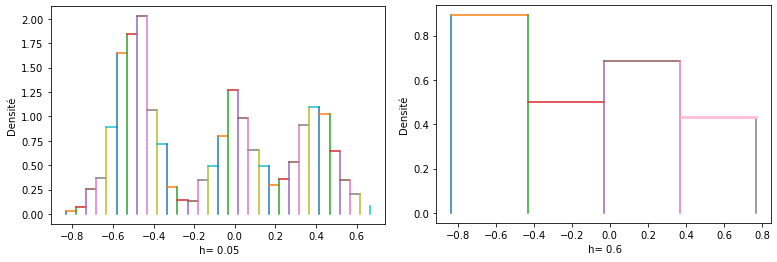
\includegraphics[width=\textwidth]{Figure 1.1.png}
  \caption{Différents histogrammes associés à un même ensemble de données avec différents paramètres de lissage}
  \label{fig:hneleveetbas}
\end{figure}
\begin{figure}[!ht]
  \centering
  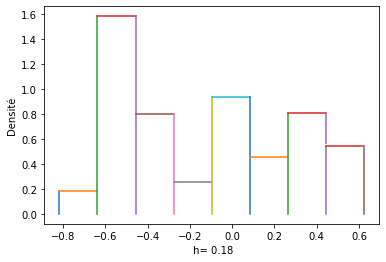
\includegraphics[width=13cm,height=8cm]{Figure 1.2.png}
  \caption{Estimation d’une densité de la probabilité par la méthode de
l’histogramme avec une valeur de pas optimal}
  \label{fig:figure2}
\end{figure}
\newpage

La figure (1.1) nous montre deux histogrammes basés sur le même ensemble de données et avec deux paramètres de lissage petit et grand. Un paramètre de lissage trop petit conduit à un histogramme plus découpé, tandis que l’autre donne un histogramme plus lisse comme le montre la figure (1.1).

\subsection{Méthode des fonctions orthogonales}
Pour cette méthode d’estimation non paramétrique, $f$ s’écrit sous la forme d’une série :
\begin{equation}
f(x) = \sum_{m=0}^{+\infty} a_m(f) e_m(x)
\end{equation}
\myequations{Equation \ref{eq:Eq12}}
Sachant que $e_m$ sont des fonctions orthogonales \newline et $a_m(f)$ les coefficients de Fourier de la densité à estimer $f$.
\newline
\newline
La méthode d’estimation consiste à tronquer la série qui s’écrit alors : 
\newline
$f_k (x)=\sum_{m=1}^k a_m (f)e_m (x)$
\newline
\newline
Puis à estimer les paramètres $(a_1 (f),...  ,a_k (f)$ , avec a$_m (f) = \int f(x) e_m (x)\,dx$, par :
\newline
${\hat a}_{m,N}=\frac{1}{N}\sum_{m=1}^{N}e_{m}(X_i)$
\section{Méthode de Noyau}
La méthode de noyau a été introduite pour la première fois par ROSENBLATT en 1956, puis développé par Parzen en 1962 pour décrire la fonction utilisée dans les méthodes non paramétriques. La méthode des noyaux consiste à associer une fonction $K(x)$ à chaque observation de l'échantillon, avec la seule restriction que son intégration sur tout le domaine de définition de $x$ doit être égale à 1. Certaines restrictions théoriques peuvent être imposées sur $K$, comme la symétrie ou la positivité sur tout le domaine de définition du noyau, mais elles sont principalement utilisées pour simplifier les développements théoriques.\newline L'estimation non paramétrique de la fonction de densité peut être vue comme la somme des fonctions $K$ de chaque observation sur tout le domaine.
\newline
Soit $K: \mathbb{R} \longrightarrow \mathbb{R}$, on dit que $K$ est un noyau si et seulement si :
\newline
$\int_{-\infty}^{\infty} K(u)du=1$
\newline
$K$ est dit positif si $K(u) \geq 0 \quad \forall u$
\newline
$K$ est dit symétrique si $K(u) = K(-u) \quad \forall u$
\newline
\newline
En pratique, les noyaux utilisés sont des noyaux d'ordre 2 ce qui implique que le noyau $K$ est lui-même une densité de probabilité. Des exemples de noyaux d'ordre 2 sont cités ci-dessous :
\begin{itemize}
    \item Le noyau rectangulaire : $K(u)=\frac{1}{2}1_{[-1,+1]}(u)$ (appelé aussi noyau de Rosenblatt)
    \item Le noyau triangulaire : $K(u)=(1-|u|)1_{[-1,+1]}(u)$
    \item Noyau d’Epanechnikov (parabolique) : $K(u)=\frac{3}{4}(1-u^2)1_{[-1,+1]}(u)$
    \item Le noyau Gaussien : $K(u)=\frac{1}{\sqrt{2\pi}}e^{-\frac{u^2}{2}}$
\end{itemize}
Les avantages des deux premières méthodes sont leur simplicité, car leur noyau est triangulaire et continu partout, ce qui permet une estimation continue. La troisième méthode est connue pour une propriété théorique d'optimalité, mais n'a pas d'importance pratique.
\newline
Voici quelques courbes de noyaux usuels présentées ci-dessous :

\begin{figure}[!ht]
  \centering
  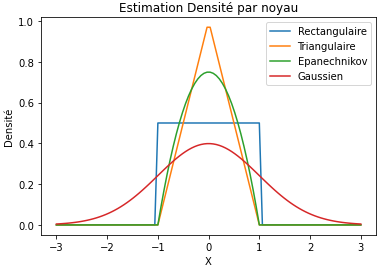
\includegraphics[width=\textwidth]{Figure 1.3.png}
  \caption{Les courbes des noyaux les plus communs}
  \label{fig:figure3}
\end{figure}

Un estimateur à noyau noté $f_n$ de la fonction $f$ est défini par : 
\begin{equation}
\hat{f}_N(x) = \frac{1}{N h_N} \sum_{i=1}^N K\left(\frac{x-X_i}{h_N}\right)
\end{equation}

\myequations{Equation \ref{eq:Eq13}}
Avec $(X_1, \dots, X_n)$ $N$ réalisations d’un échantillon et $K$ une densité de probabilité appelée noyau (Voir les exemples cités dans la partie précédente et \shortcite{parzen1962} pour une revue plus exhaustive). Ainsi, le noyau $K$ est centré sur le point $x$ dont on veut estimer l’image par $f$ : il s’agira de sommer les contributions des différents $x_i$ en normalisant par l’entité $h_N$ appelée "paramètre de lissage" ou plus simplement "pas".

\subsection{Description de l’estimateur à noyau }
Les différentes étapes de l'algorithme Plug-in sont détaillées ci-dessous :

\begin{enumerate}
\item \textbf{ Choix du noyau :}
Le choix du noyau dépend du problème à résoudre. Il existe plusieurs types de noyaux comme nous l'avons vu dans la partie précédente.

\item \textbf{ Fixation du paramètre de lissage :}
Cette étape est très importante, dans les parties suivantes nous allons voir les algorithmes qui vont nous aider à choisir le pas optimal.

\item \textbf{ Placement des noyaux sur les données :}
Pour chaque point de données, un noyau est placé autour de ce point. La forme et la taille du noyau dépendent du choix de noyau et du pas.

\item \textbf{ Normalisation de la densité de probabilité estimée :}
Pour que la densité de probabilité estimée puisse être interprétée comme une probabilité, elle doit être normalisée. Cela signifie que l'aire sous la courbe de densité de probabilité doit être égale à 1.

\item \textbf{Interprétation de la densité de probabilité estimée.}
\end{enumerate}
Les différentes étapes citées sont schématisées dans la figure 1.4 : 
\begin{figure}[!ht]
  \centering
  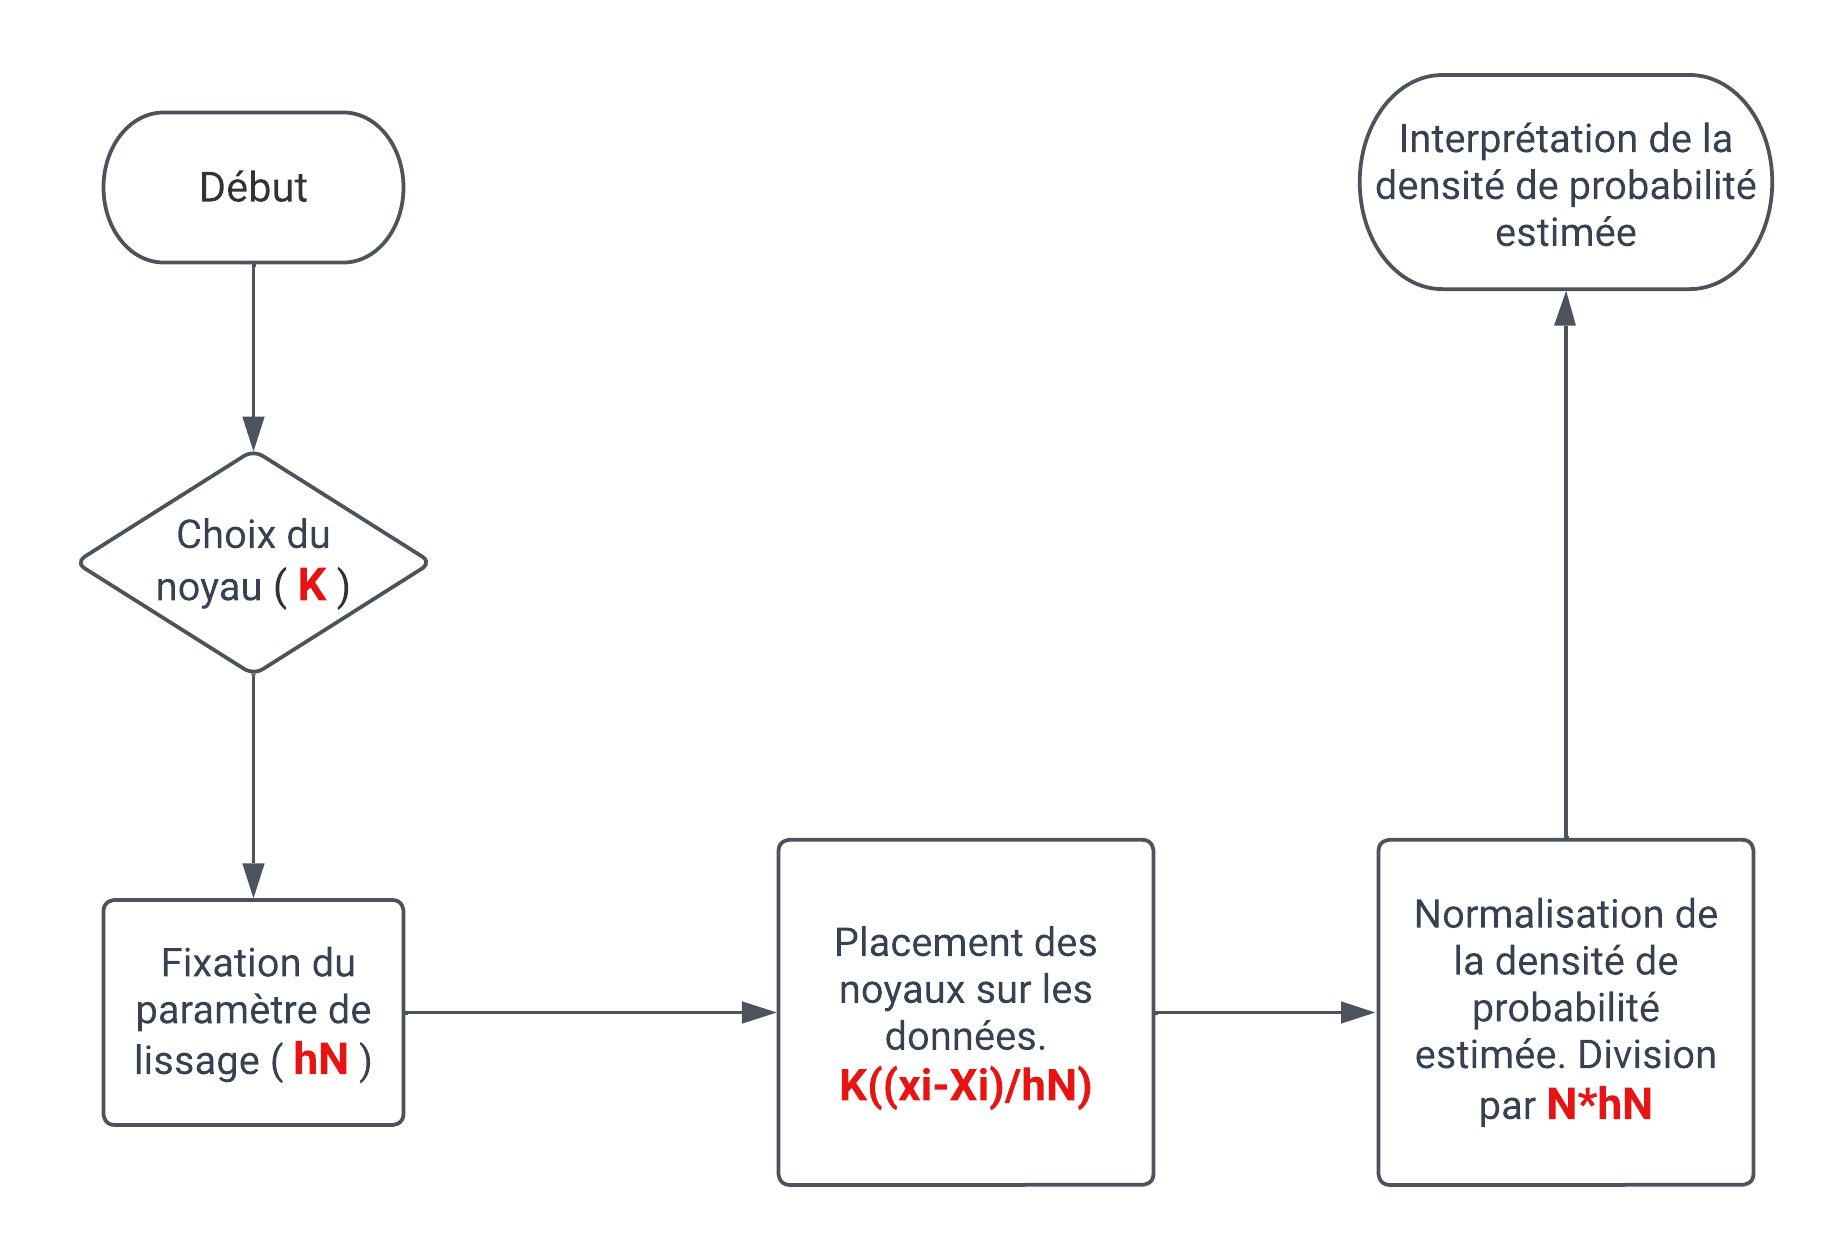
\includegraphics[width=14cm,height=10cm]{Figure 1.4.png}
  \caption{Schéma descriptif de l'estimateur à noyau}
  \label{fig:Schéma descriptif de l'estimateur à noyau}
\end{figure}
\newpage
Voici une implémentation en Python 3 de l'estimateur de noyau, permettant d’estimer la densité de probabilité d'un ensemble de données $X$ : \\
\begin{lstlisting}
X = generation_LN(m, s, n) 
P = 100
c = (2 * np.pi)**0.5
for NBI in range(1,10):
    hn = #valeur optimale
    valeur=2*2.23*(hn)**(-6)/500;
    Y = []
    Yk = []
    for k in range(P):
        yk = mini + (maxi-mini)*k/P
        Y.append(0)
        Yk.append(yk)
        for i in range(1,n):
            z = (yk-X[i]) / hn
            z = z**2
            z = -0.5*z
            z = np.exp(z)
            Y[-1] += z
        Y[-1] = Y[-1] / (c*n*hn)
    e = -100
        d = 100
    I = 0
    z = 0
    for k in range(1, P-2):
        z = (Y[k+1]-2*Y[k]+Y[k-1])
        I += z**2
    I = I + ((Y[P-2])**2 + (Y[P-2]-2*Y[P-3])**2) / (r**4)
return Y

\end{lstlisting}
Avec : \\
Les paramètres de la loi normale à générer sont $m$, $s$ et $n$ ( moyenne, écart-type, taille).
\newpage
\subsection{Paramètre de lissage}
Le choix des paramètres de lissage dans les méthodes du noyau pour estimer la densité de probabilité est un aspect important de ces méthodes. Le paramètre de lissage, également appelé paramètre de bande passante, contrôle la largeur du noyau utilisé pour lisser les données. Un paramètre de lissage plus élevé entraînera une estimation plus lisse de la densité de probabilité, mais pourrait masquer certains détails importants dans les données (Figure 1.5).\\ Un paramètre de lissage plus faible permettra une estimation plus détaillée de la densité de probabilité, mais pourrait entraîner une estimation plus bruitée (Figure 1.6). Il est donc important de trouver un compromis approprié entre le lissage et la résolution lors de la sélection des paramètres de lissage.
\begin{figure}[!ht]
  \centering
  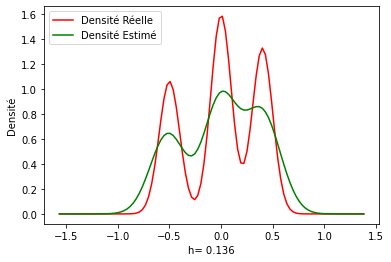
\includegraphics[width=13cm,height=10cm]{Figure 1.5.png}
  \caption{$h_N$  Élevé }
  \label{fig:$h_N$  Élevé}
\end{figure}
\begin{figure}[!ht]
  \centering
  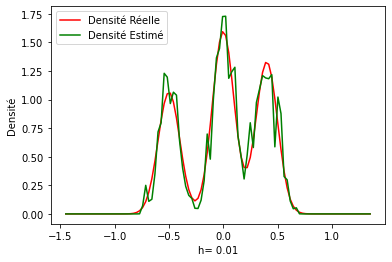
\includegraphics[width=13cm,height=8cm]{Figure 1.6.png}
  \caption{$h_N$  Faible }
  \label{fig:$h_N$  Faible}
\end{figure}
\begin{figure}[!ht]
  \centering
  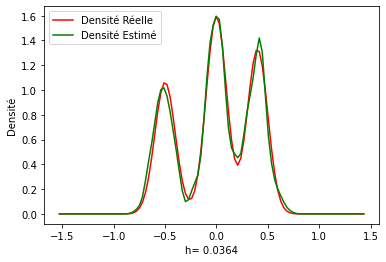
\includegraphics[width=13cm,height=8cm]{Figure 1.7.png}
  \caption{$h_N$  Optimal }
  \label{fig:$h_N$  Optimal}
\end{figure}
\newpage

L’estimation de la densité nécessite également le choix adéquat du paramètre de lissage $h_N$ , et pour cette valeur idéale, nous obtenons une allure qui suit parfaitement la vraie distribution. (Figure 1.7)
\section{Étude de la convergence}
L’étude théorique de la convergence de ${\hat f}_n$ (Densité estimée) vers $f$(Densité réelle) permet de formuler expression de $h_N$  optimal et de déterminer le noyau optimal censé à aboutir meilleure estimation.
Ainsi, évaluation de EQM mesure la différence entre densité estimée et densité réelle.
\begin{equation}
EQM=\text{var}({\hat f}_{n}) + \left(f - E[{\hat f}_n]\right)^2
\end{equation}
\myequations{Equation \ref{eq:Eq14}}
En minimisant EQM, nous obtiendrons l’expression analytique de la valeur optimale de $h_N$ notée $h^*_N$ comme suit : 
\begin{equation}
\fbox{\boldmath{$\displaystyle h^*_N = N^{-\frac{1}{5}} \cdot (J(f))^{-\frac{1}{5}} \cdot (M(K))^{\frac{1}{5}}
$}}
\end{equation}
\myequations{Equation \ref{eq:Eq14}}
Avec : 
\begin{align}
 J(f) &= \int_{-\infty}^{\infty} (f''(x))^2 \,dx \\ M(K) &= \int_{-\infty}^{\infty} K^2(u) \, du
\end{align}

$f''$  étant la dérivée seconde de $f$

L’expression théorique du paramètre de lissage optimal au sens de l'EQM dépend de la taille de l’échantillon $N$, de l’intégrale du noyau choisi élevé au carré $M(K)$ ainsi que de l’intégrale de la dérivée seconde élevée au carré de ${\hat f}_N$ notée $J(f)$. La valeur de $M(K)$, liée au noyau choisi, est facilement déduite analytiquement ou numériquement. Par contre, l’entité $J(f)$  ne peut être directement approchée puisqu’elle est liée à $f$, fonction inconnue à estimer.

\subsection{Optimisation de $J(f)$}
L'étude de la convergence de l'estimateur à noyau a permis de formuler l'expression théorique pour le pas optimal $h^*_N$. Cependant, il est difficile d'estimer l'intégrale de la dérivée seconde élevée au carré de la densité à estimer, appelée $J(f)$ . Pour résoudre ce problème, plusieurs méthodes ont été développées, telles que les méthodes ROT \shortcite{silverman1986, hardle1991smoothing,terrell1990variable} , cross-validation \shortcite{bowman1984,hall1987,Scott1987,Simon1991}, Plug-in \shortcite{hall1987,park1990} et la méthode des contrastes \shortcite{mugadi2004}. Ces méthodes cherchent à minimiser EQM en sélectionnant les paramètres de lissage optimaux. Nous allons voir par la suite les méthodes : LSCV, ROT et PLUG-IN et les comparer. 

\subsubsection{LSCV}
Simon Sheather a développé la méthode d'optimisation LSCV dans le contexte de l'estimation de densité au début des années 1991. L'idée de Sheather était d'utiliser la validation croisée\shortcite{bates2023crossvalidation} pour estimer le paramètre de largeur de bande optimal pour une estimation de densité de noyau. La méthode LSCV divise l'ensemble de données en deux parties, une partie pour l'estimation de densité et l'autre pour la validation. La partie de validation est utilisée pour calculer une fonction de perte, qui mesure l'erreur entre l'estimation de densité et les données observées. Le paramètre de largeur de bande qui minimise la fonction de perte est choisi comme le paramètre optimal pour l'estimation de densité.
\newline
\textbf{Sheather} a présenté la méthode LSCV et a montré qu'elle avait plusieurs avantages par rapport aux méthodes existantes de sélection de largeur de bande. En particulier, LSCV était plus robuste au choix de la fonction de noyau et pouvait être utilisé avec plusieurs fonctions de noyau, y compris celles qui n'étaient pas lisses ou symétriques.
Depuis la publication de l'article de Sheather, LSCV est devenu une méthode largement utilisée de sélection du paramètre de lissage dans le domaine de l'estimation de densité, et a été appliqué dans de nombreux contextes différents, notamment le traitement du signal, l'analyse d'image et la finance.
\begin{equation}
lscv(h)=\int \hat{f_{h^2}} - \frac{2}{n} {\sum_{i=1}^{n}{\hat f}_{-i}}(Xi)
\end{equation}
\myequations{Equation \ref{eq:Eq18}}
Voici une implémentation en Python 3 de la méthode LSCV : 
\begin{lstlisting}
import numpy as np
from sklearn.model_selection import GridSearchCV
#Mettre en place la grille des pas a explorer
param_grid = {'bandwidth': np.logspace(-1, 1, 20)}
#Utiliser GridSearchCV pour trouver le pas optimal
grid = GridSearchCV(KernelDensity(kernel='gaussian'), param_grid=param_grid, cv=10)
grid.fit(X[:, None])
hn_Optimal= grid.best_estimator_.bandwidth
\end{lstlisting}

\subsubsection{ROT}
La méthode de Silverman, nommée d'après le statisticien \textbf{David Silverman}, est une méthode non paramétrique utilisée pour estimer les fonctions de densité de probabilité. Elle a été introduite pour la première fois en 1986 dans un article intitulé \textbf{"Density Estimation for Statistics and Data Analysis"}. La méthode est largement utilisée dans l'analyse statistique et l'apprentissage automatique pour estimer les fonctions de densité de probabilité en raison de sa simplicité et de sa précision.

La méthode de Silverman repose sur l'hypothèse que la fonction de densité de probabilité sous-jacente est lisse et peut être approximée à l'aide d'une distribution gaussienne. La formule pour la méthode de Silverman consiste à sélectionner une largeur de bande optimale pour l'estimateur de densité de noyau gaussien en fonction des données disponibles. La largeur de bande optimale est choisie pour équilibrer le compromis entre la sur-lissage et le sous-lissage.

La méthode a été largement citée et appliquée dans divers domaines tels que l'économétrie, la finance et l'ingénierie. En fait, c'est la méthode implémentée par défaut dans la bibliothèque de KDE gaussien en Python. La méthode a également été étendue pour gérer les données multivariées et pour incorporer d'autres types de noyaux. Dans l'ensemble, la méthode ROT a été une contribution significative au domaine de l'estimation de densité non paramétrique et reste un outil important pour l'analyse des données.

Silverman a commencé par la formule de l'AMISE\footnote{L’AMISE fournit une mesure de l’efficacité d’un estimateur, et il est souvent utilisé pour comparer différents estimateurs en termes de performance à mesure que la taille de l’échantillon augmente.}  d'un estimateur $KDE$, qui implique la fonction de densité réelle $f(x)$  et la fonction noyau $K(x$) :
\begin{equation}
AMISE = \frac{1}{4} \int \frac{f''(x)^2}{[K(x)]^2} h^4 dx + \frac{1}{nh} \int [K(u)]^2 du
\end{equation}
\myequations{Equation \ref{eq:Eq19}}
Où $h$ est le paramètre de bande, n est la taille de l'échantillon et $f''(x)$ désigne la deuxième dérivée de $f(x)$ .

Silverman a ensuite fait deux hypothèses simplificatrices :
\begin{enumerate}
\item Il a supposé que la fonction noyau $K(x)$  est une distribution normale standard, ce qui signifie que l'intégrale de $K(u)^2$  sur son support est égale à $1$.
\item Il a supposé que la vraie fonction de densité $f(x)$  est lisse, ce qui signifie que sa deuxième dérivée est bornée.
\end{enumerate}

Sous ces hypothèses, le deuxième terme de la formule AMISE devient une constante, et Silverman s'est concentré sur la minimisation du premier terme par rapport à $h$ .En différenciant le premier terme par rapport à $h$ et en le fixant à zéro, il a obtenu la formule suivante pour le paramètre de bande optimal :
\begin{equation}
h_{Optimal} = 1.06 . \hat{\sigma} .  n^{\frac{-1}{5}}\end{equation}
\myequations{Equation \ref{eq:Eq20}}
Où  $\hat{\sigma}$ est l'écart-type de l'échantillon des données. Cette formule est connue sous le nom de règle de Silverman et elle fournit une méthode simple et pratique pour sélectionner le paramètre de bande dans KDE.

Voici une implémentation en Python 3 de la méthode ROT : 
\begin{lstlisting}
from scipy.stats import gaussian_kde
import numpy as np

kde = gaussian_kde(X)
evaluated = np.linspace(a, b, n)
density = kde(evaluated)

\end{lstlisting}
Comme nous l'avons précédemment dit ROT est la méthode implémentée par défaut dans la bibliothèque de KDE gaussien en Python.

\subsubsection{Plug-in}
Cette méthode fait appel à un algorithme itératif pour la recherche du pas optimal.

Le principe commence par un choix aléatoire de $J(f)$, ensuite les évaluations de $J(f)$  sont déduites à partir de la première valeur. Plusieurs itérations faites permettent de converger vers le paramètre de lissage optimal.

Étapes : 
\begin{enumerate}
    \item 	Détermination analytique de $M(K) $
	\item Choix arbitraire de $J_0(f)$, qui permet de la déduction de$h_N^0$
	\item Estimation de $f$ par la méthode de noyau en utilisant le paramètre de lissage $h_N^0$.\\Généralement cette première valeur, notée $f_0$, ne converge pas vers $f$.
	\item Ré-estimation de $J_k(f)$ en utilisant la dérivée seconde de ${\hat f}_{(k-1)}$ puis en l’intégrant. $h_N(k)$ est déduite à chaque itération.
	\item Arrêt de l’algorithme lorsque la différence entre $h_N^k$ et $h_N^{k-1}$ est relativement faible.

\end{enumerate}
Voici une implémentation en Python 3 de la méthode PLUG-IN à l’aide de l’estimateur de noyau : 
\begin{lstlisting}
def gitkernel(X,mini,maxi,r):
    P = 100
    P0 = 2000
    e = -100
    d = 100
    c = (2 * np.pi)**0.5
    I = 0
    for k in range(1, P0+1):
        zk = e + (d-e) * k/P0
        u = np.exp(-(zk**4)/4)
        I += u
    MK = I * (d-e) / (c*c*P0)
    Jf = 1
    n = len(X)


    for NBI in range(1,10):
        #Estimation de hN
        hn = (MK**0.2) * (Jf*n)**(-0.2)
        valeur=2*2.23*(hn)**(-6)/500;
        Y = []
        Yk = []
        for k in range(P):
            yk = mini + (maxi-mini)*k/P
            Y.append(0)
            Yk.append(yk)
            for i in range(1,n):
                z = (yk-X[i]) / hn
                z = z**2
                z = -0.5*z
                z = np.exp(z)
                Y[-1] += z
            Y[-1] = Y[-1] / (c*n*hn)
        e = -100
        d = 100
        I = 0
        Jf = 0
        z = 0
        for k in range(1, P-2):
            z = (Y[k+1]-2*Y[k]+Y[k-1])
            I += z**2
        I = I + ((Y[P-2])**2 + (Y[P-2]-2*Y[P-3])**2) / (r**4)
        #Estimation de Jf 
        Jf = I / (r**3)
        
    return Y


\end{lstlisting}

\section{Méthode de noyau difféomorphisme}
La méthode de noyau peut causer des problèmes (Effet de Gibbs) lorsque les observations sont rares aux bords de la plage, ce qui peut entraîner une sous-estimation de la densité de probabilité.
La solution consiste au changement de variable par un difféomorphisme $C^1$(Classe 1), qui nous aide à éliminer l’effet de Gibbs et bien estimer la densité.

Ensuite, nous introduisons un nouvel algorithme itératif pour l’ajustement de la valeur du paramètre de lissage. Le proposé algorithme, que nous appellerons Plug-in-difféomorphisme, s’inspire de l’algorithme Plug-in conventionnel lequel est adapté à cet estimateur.

Cette généralisation du Plug-in conventionnel nécessite une double initialisation ce qui rend sa convergence moins aisée.
L’expression de l’estimateur noyau difféomorphisme :
\begin{equation}
{\hat f}(x)= \frac{\left | \varphi '(x))  \right |}{Nh_N}\sum_{i=1}^{N}K(\frac{\varphi (x) - \varphi(X_i)}{h_N})
\end{equation}
\myequations{Equation \ref{eq:Eq21}}
Avec $\varphi$ est un $C^1$  difféomorphisme qui a pour limite l’infini lorsque $x$ tend vers $a$ ou $b$.

Exemple de $C^1$  difféomorphisme :
\newline
\begin{equation}
    \begin{cases}
\varphi _{a,b} : ]a,b[ \longrightarrow \mathbb{R} \\ x\longrightarrow log(\frac{x-a}{b-x})
\end{cases}
\end{equation}
\myequations{Equation \ref{eq:Eq22}}

Le choix du meilleur difféomorphisme a été effectué selon les valeurs de l’erreur quadratique moyenne qui doit être la plus faible possible.

\subsection{Optimisation du paramètre de lissage $(J_\phi (f)))$ : \\Plug-in Difféomorphisme }
La complexité de l'optimisation des paramètres de lissage pour la méthode de noyau \\difféomorphisme est accrue par l'utilisation de l'algorithme Plug-in, car$M_\phi(K)$ dépend de la densité de probabilité inconnue $f$, et $J_\phi(f)$ qui dépend de $f$,$f'$ et $f''$.\\En comparaison, l'algorithme Plug-in conventionnel utilise une constante $M(K)$ et $J(f)$ qui ne dépend que de $f''$.

En posant :		

$M_{\phi (K)} = M(K) \int _R \left|\varphi '(x) \right| f(x) \, dx$ 
\newline
et 
\newline
$J_{\phi}(f) = \int_{R} \frac{F^2 (x)}{[\varphi'(x)]^8} \, dx$
\newline
Il est possible de déduire la valeur de $h_N$ qui minimise l’EQM, que l’on notera $h^*_N$.

\begin{equation}
h^*_N = [M_\phi (K)]^\frac{1}{5} [J_\phi (f)]^\frac{-1}{5} N^\frac{-1}{5}
\end{equation}
\myequations{Equation \ref{eq:Eq23}}

Étapes:
\begin{enumerate}
    \item Initialisation arbitraire de $M_\phi^0 (K)$
    \item Initialisation arbitraire de $J_\phi^0 (K)$,  $h_N^0$ est déduite.
    \item Estimation de $f^0$ 
    \item A la $k^{eme}$ itération une approximation des différentes quantités :$ M_\phi (K)$ , ${f^{(k)}}' et {f^{(k)}}''$
    \item Estimation de $J_\phi$ $f^k$ ainsi de $h_N^k$
	\item Approximation de $f^{(k)}$  
	\item Arrêt de l’algorithme lorsque la différence entre $h_N^k$ et $h_N^{(k-1)}$ devient relativement faible.

\end{enumerate}
\newpage

\section{Conclusion}
	 Dans ce chapitre, nous avons commencé par expliquer la densité de probabilité et comment l’estimer, soit par des méthodes paramétriques ou non-paramétrique. Nous avons présenté les différentes méthodes non-paramétriques, mais nous nous sommes focalisés sur les estimateurs noyau, et par une étude de convergence nous avons bien minimisé le EQM et nous avons trouvé la fonction optimale du paramètre de lissage, en utilisant l’algorithme plug-in qui permet de converger la densité estimée vers la densité réelle. 

Après, nous avons introduit la méthode noyau difféomorphisme et l’algorithme plug-in difféomorphisme pour une meilleure estimation des distributions à supports bornés ou semi-bornés. Cette méthode présente l’avantage de minimiser de manière remarquable le phénomène de Gibbs. Mais nous avons constaté une augmentation de complexité de l’algorithme qui sert à l’optimisation de paramètre de lissage, algorithme Plug-in.

\clearpage

\chapter{Machine Learning}
\section{Introduction}
L'apprentissage automatique est une discipline de l'informatique qui vise à développer des mod-\\èles capables d'apprendre à partir de données pour effectuer des tâches spécifiques. Le deep learning est une approche récente en apprentissage automatique, qui consiste à utiliser des réseaux de neurones profonds dans l'objectif de modéliser des représentations de données complexes. Les réseaux de neurones convolutifs (CNN) sont une architecture de réseaux de neurones profonds adaptée à la reconnaissance d'images.

Dans ce chapitre, nous allons explorer l'état de l'art du machine learning en nous concentrant sur les réseaux de neurones convolutifs. Nous allons commencer par examiner les bases théoriques de l'apprentissage automatique, en expliquant les concepts de classification, de régression et de clustering. Nous aborderons ensuite les différents types d'apprentissage automatique, notamment l'apprentissage supervisé et l'apprentissage non supervisé.

Nous passerons ensuite en revue les principales architectures des réseaux de neurones utilisés dans le domaine du deep learning, en nous focalisant sur les CNN. Nous détaillerons les diff-\\érentes couches de neurones qui composent ces architectures, telles que les couches de convolution, les couches de pooling et les couches de sortie. Nous discuterons ensuite des hyperparamètres couramment utilisés pour entraîner ces modèles, tels que le taux d'apprentissage, le nombre d'époques et la taille du lot. 

Enfin, nous discuterons d'un défi spécifique de l'apprentissage automatique, à savoir comment optimiser les hyperparamètres. Aussi, nous avons illustré notre propos en nous focalisant sur l'optimisation du nombre d'époques.

\section{Intelligence artificielle}
IA est une branche large de l'informatique qui s'intéresse à la construction de machines intelligentes capables d'effectuer des tâches qui nécessitent habituellement une intelligence humaine. C'est un domaine qui combine les sciences de l'informatique et les mathématiques afin de pouvoir modéliser des problèmes de la vie courante puis d’implémenter des algorithmes pouvant résoudre ces problèmes avec un taux de réussite élevé.


\section{Machine Learning}
L'apprentissage automatique est la science de programmer les ordinateurs de sorte qu'ils puissent apprendre à partir des données.
L'apprentissage automatique est avant tout basé sur les données, qui sont la clé de voûte de tout algorithme d'apprentissage automatique. Les algorithmes d'apprentissage automatique sont conçus pour extraire des informations et des modèles à partir de grandes quantités de données, en utilisant des techniques statistiques et mathématiques sophistiquées pour optimiser des modèles permettant de donner des réponses appropriées à une problématique donnée. les données ou une partie de ces données sont utilisés pour entraîner les algorithmes et optimiser les modèles.

La taille des bases de données pour les problèmes actuels est extrêmement élevée, ce qui rend leur utilisation difficile en raison de la complexité de la représentation de ces données dans l'espace. Leur utilisation nécessite généralement des traitements préalables pour les nettoyer et les homogénéiser. Souvent, ces données sont assimilées à des variables aléatoires multivariées, ce qui implique la manipulation d'espaces de dimensions élevées. Des méthodes de réduction de dimensions peuvent améliorer les performances des algorithmes utilisés en les faisant passer vers un espace de dimension beaucoup moins élevée.\\
Les données sont divisées en deux catégories : labellisées ou non-labellisées.
\subsection{Apprentissage supervisé}
Dans l’apprentissage supervisé, les données utilisées sont étiquetées ou labellisées, c’est-à-dire que leurs appartenances sont connues.

Les problèmes de classification et de régression sont des exemples courants de tâches d'apprentissage supervisé.
\newpage
\begin{figure}[!h]
  \centering
  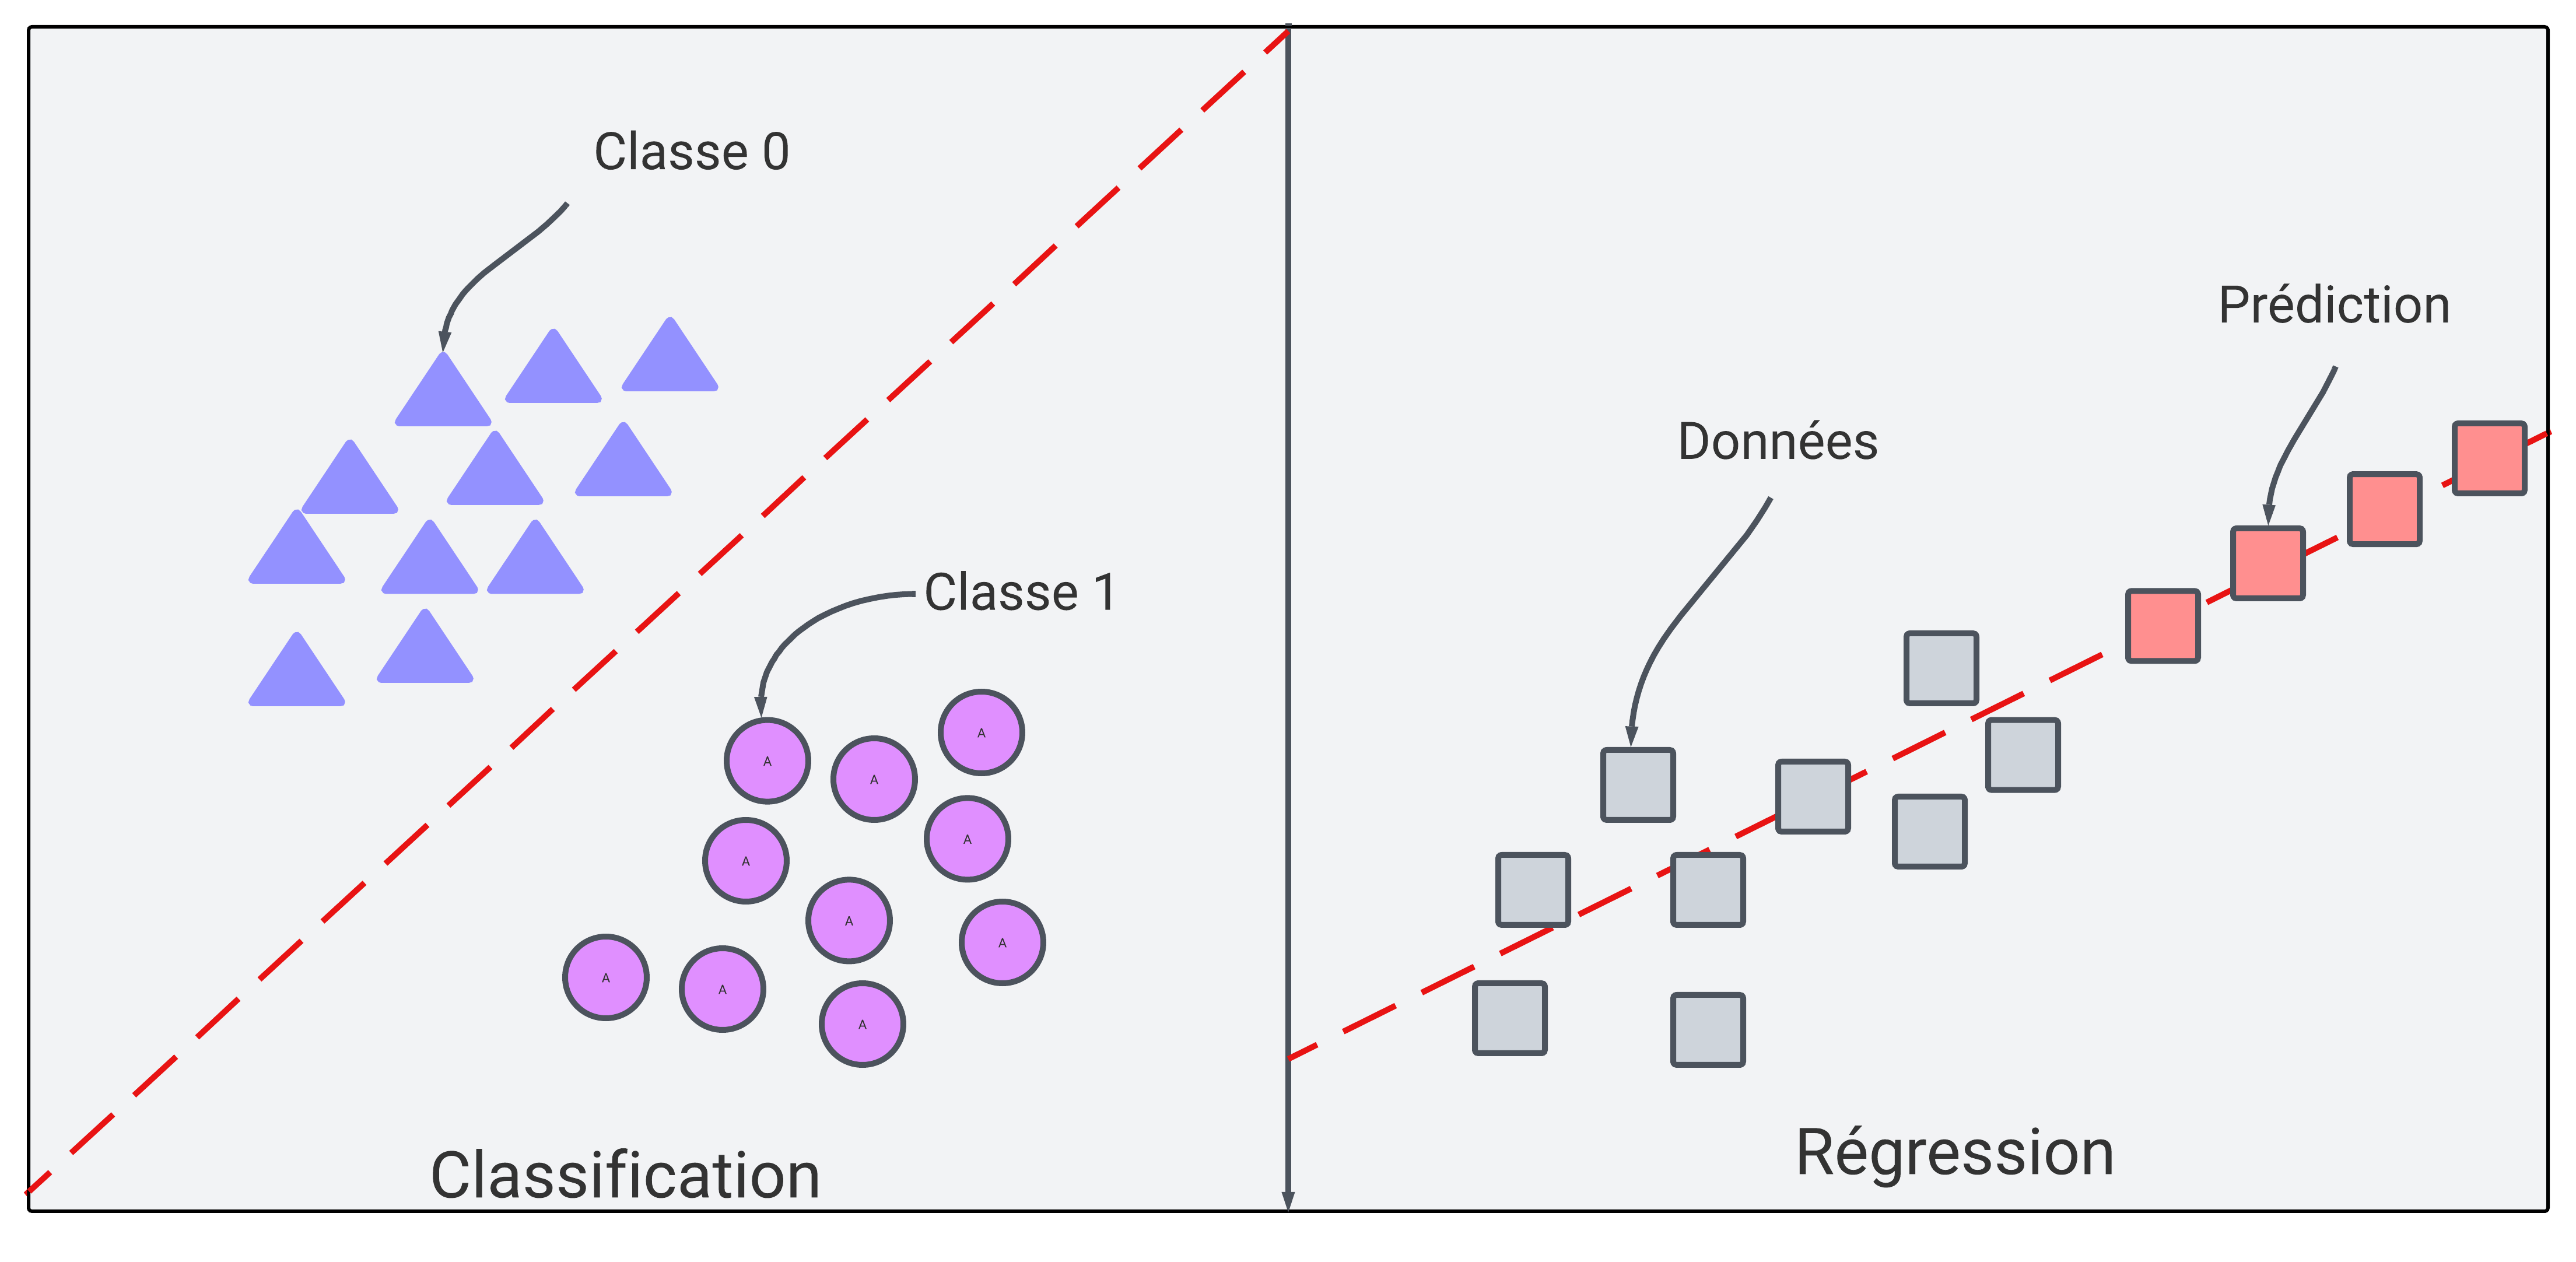
\includegraphics[width=\textwidth]{Figure 2.1.png}
  \caption{Modèles de classification et de régression}
  \label{fig:Modèles de classification et de régression}
\end{figure}



Parmi les algorithmes d’apprentissage supervisé, nous citons : 
\begin{itemize}
   \item[$\bullet$]KNN, SVM, Naïve Bayes, Arbre de décision pour la classification.
    \item[$\bullet$]Régression linéaire ou logistique pour la régression.
   \item[$\bullet$]Les réseaux de neurones pour les deux.
\end{itemize}

\subsection{Apprentissage non-supervisé}
L'apprentissage non-supervisé est une méthode de machine learning où il n'y a pas d'informations préalables sur l'appartenance ou le nombre de classes dans les données d'entraînement. Contrairement à l'apprentissage supervisé, il n'y a pas de labels associés à chaque exemple de données, ce qui signifie que l'algorithme doit trouver des modèles de similitude ou de différence entre les données pour les regrouper en clusters ou les transformer en représentations plus simples et compréhensibles.

Un exemple courant de cette approche est le clustering, qui consiste à regrouper les échantillons similaires en classes ou en groupes (Figure 2.2).
\newpage
\begin{figure}[!h]
  \centering
  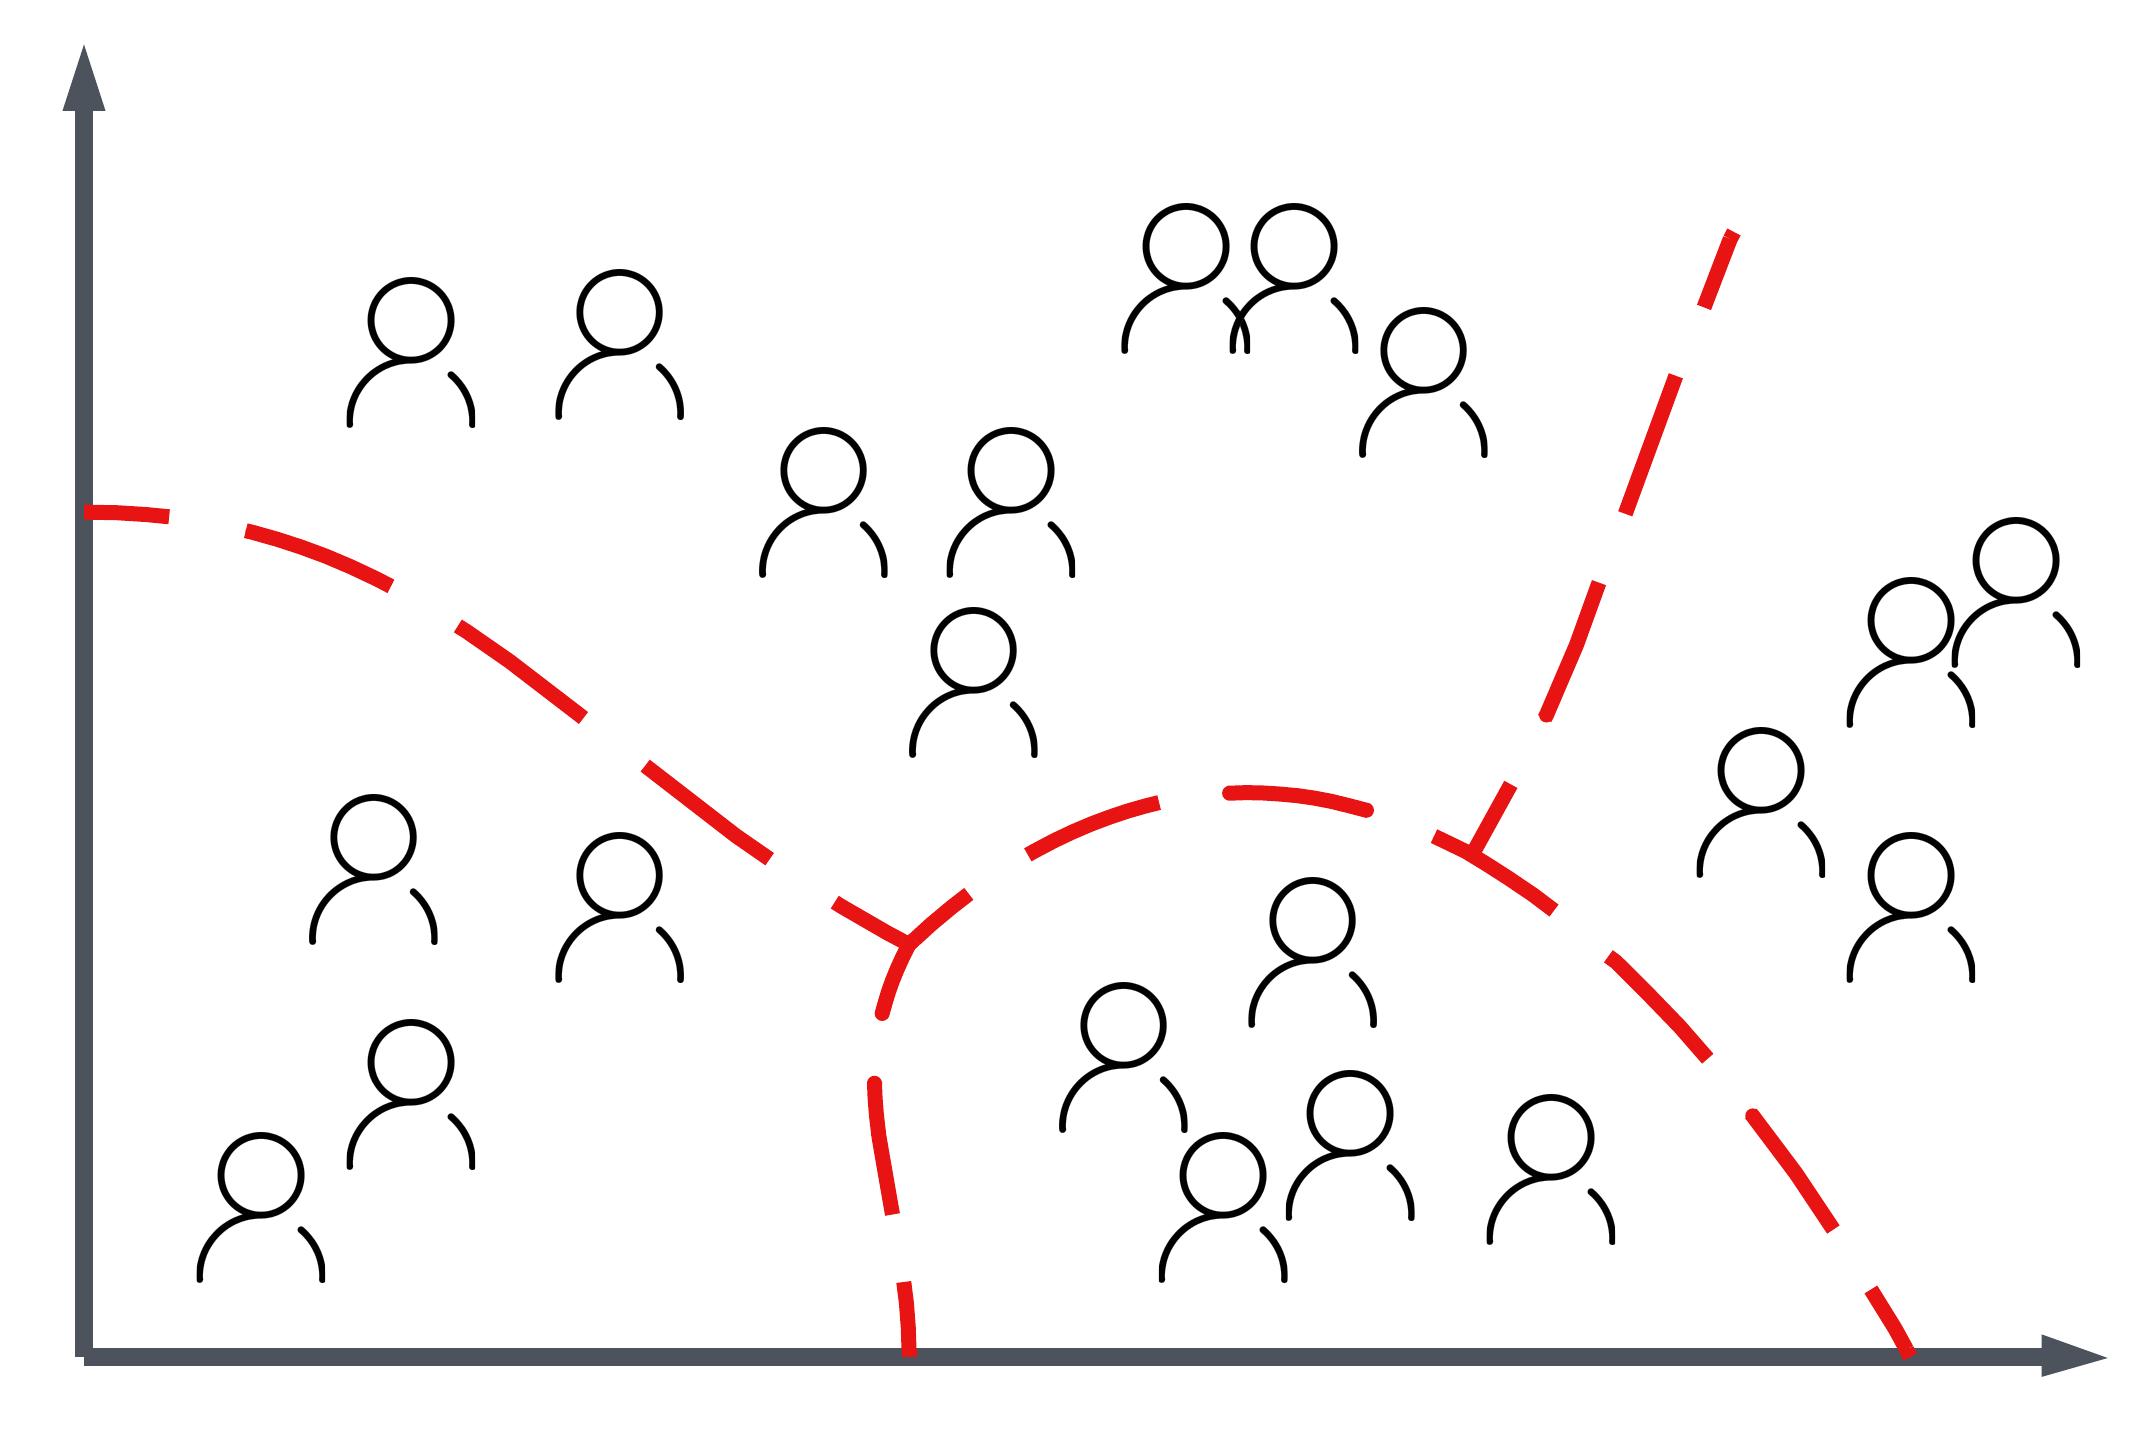
\includegraphics[width=9cm,height=6cm]{Figure 2.2.png}
  \caption{Clustering}
  \label{fig:Clustering}
\end{figure}

Il est également important de souligner que la réduction de dimensions est une étape cruciale pour simplifier les modèles des algorithmes d'apprentissage automatique. L'analyse en composantes principales (ACP) est un exemple d'une technique de réduction de dimensions permettant de passer d'un espace de haute dimension à un espace de dimension réduite, généralement deux ou trois dimensions. Cela permet de visualiser les données de manière plus simple et d'identifier des tendances ou des relations entre les variables qui seraient autrement difficiles à percevoir dans un espace de grande dimension.

Dans la figure 2.3, les attributs des chiffre manuscrits de la base MNIST sont projetées sur 2 axes principaux suite à l'utilisation de l'ACP.
\begin{figure}[!h]
  \centering
  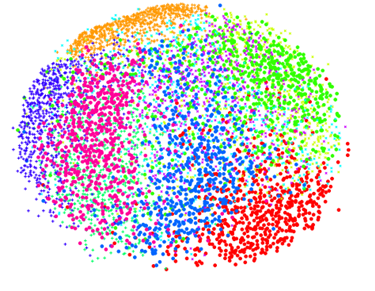
\includegraphics[width=8cm,height=6cm]{Figure 2.3.png}
  \caption{Visualisations des 6000 chiffres manuscrits de la BD MNIST}
  \label{fig:Visualisations des 6000 chiffres manuscrits de la BD MNIST}
\end{figure}
\newpage
\subsection{Apprentissage semi-supervisé}
L'apprentissage semi-supervisé consiste à travailler avec des bases de données où seule une partie des données est étiquetée. Les algorithmes utilisent la similarité entre les données étiquetées et non étiquetées pour regrouper les échantillons dans des classes similaires. Cette approche est intéressante car elle permet de tirer parti de la puissance de l'apprentissage supervisé tout en évitant les coûts élevés liés à l'étiquetage manuel de grandes quantités de données. (Figure 2.4)
\begin{figure}[!h]
  \centering
  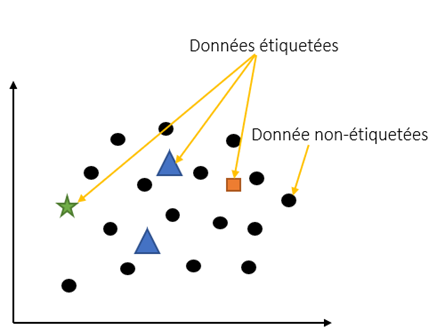
\includegraphics[width=10cm,height=8cm]{Figure 2.4.png}
  \caption{Exemple des données d’entrée pour un algorithme semi-supervisée}
  \label{fig:Exemple des données d’entrée pour un algorithme semi-supervisée}
\end{figure}

\subsection{Apprentissage par renforcement}
L’apprentissage par renforcement est une branche de l'apprentissage automatique qui se concentre sur la prise de décision séquentielle. Dans cette approche, un algorithme apprend à partir de l'interaction avec son environnement en effectuant des actions et en recevant des récompenses ou des pénalités en fonction de la qualité de ses décisions. L'objectif est d'apprendre à prendre les meilleures décisions possibles dans un environnement dynamique et incertain, en maximisant une récompense à long terme.
\clearpage
\section{Apprentissage profond(Deep Learning)}
Le Deep Learning utilise des réseaux de neurones artificiels très profonds pour effectuer des tâches de classification, de prédiction et de génération de données. Les réseaux de neurones profonds sont des réseaux qui ont de nombreuses couches cachées, ce qui leur permet de capturer des relations complexes et non linéaires entre les données d'entrée et de sortie. \\

\begin{itemize}
   \item[$\bullet$]\textbf{Couche d’entrée} : Cette Couche contient les entrées : Texte, valeurs numériques, images...
    \item[$\bullet$]\textbf{Couche cachée} :  Cette couche trouve une relation entre la couche d’entrée et celle de sortie. Le choix de nombre de couches cachées est fait selon a complexité du problème.
     \vspace{0.5em}
   \item[$\bullet$]\textbf{Couche de sortie} : Cette couche est la dernière couche de neurones qui génère les sorties de données.
\end{itemize}

\begin{figure}[!h]
  \centering
  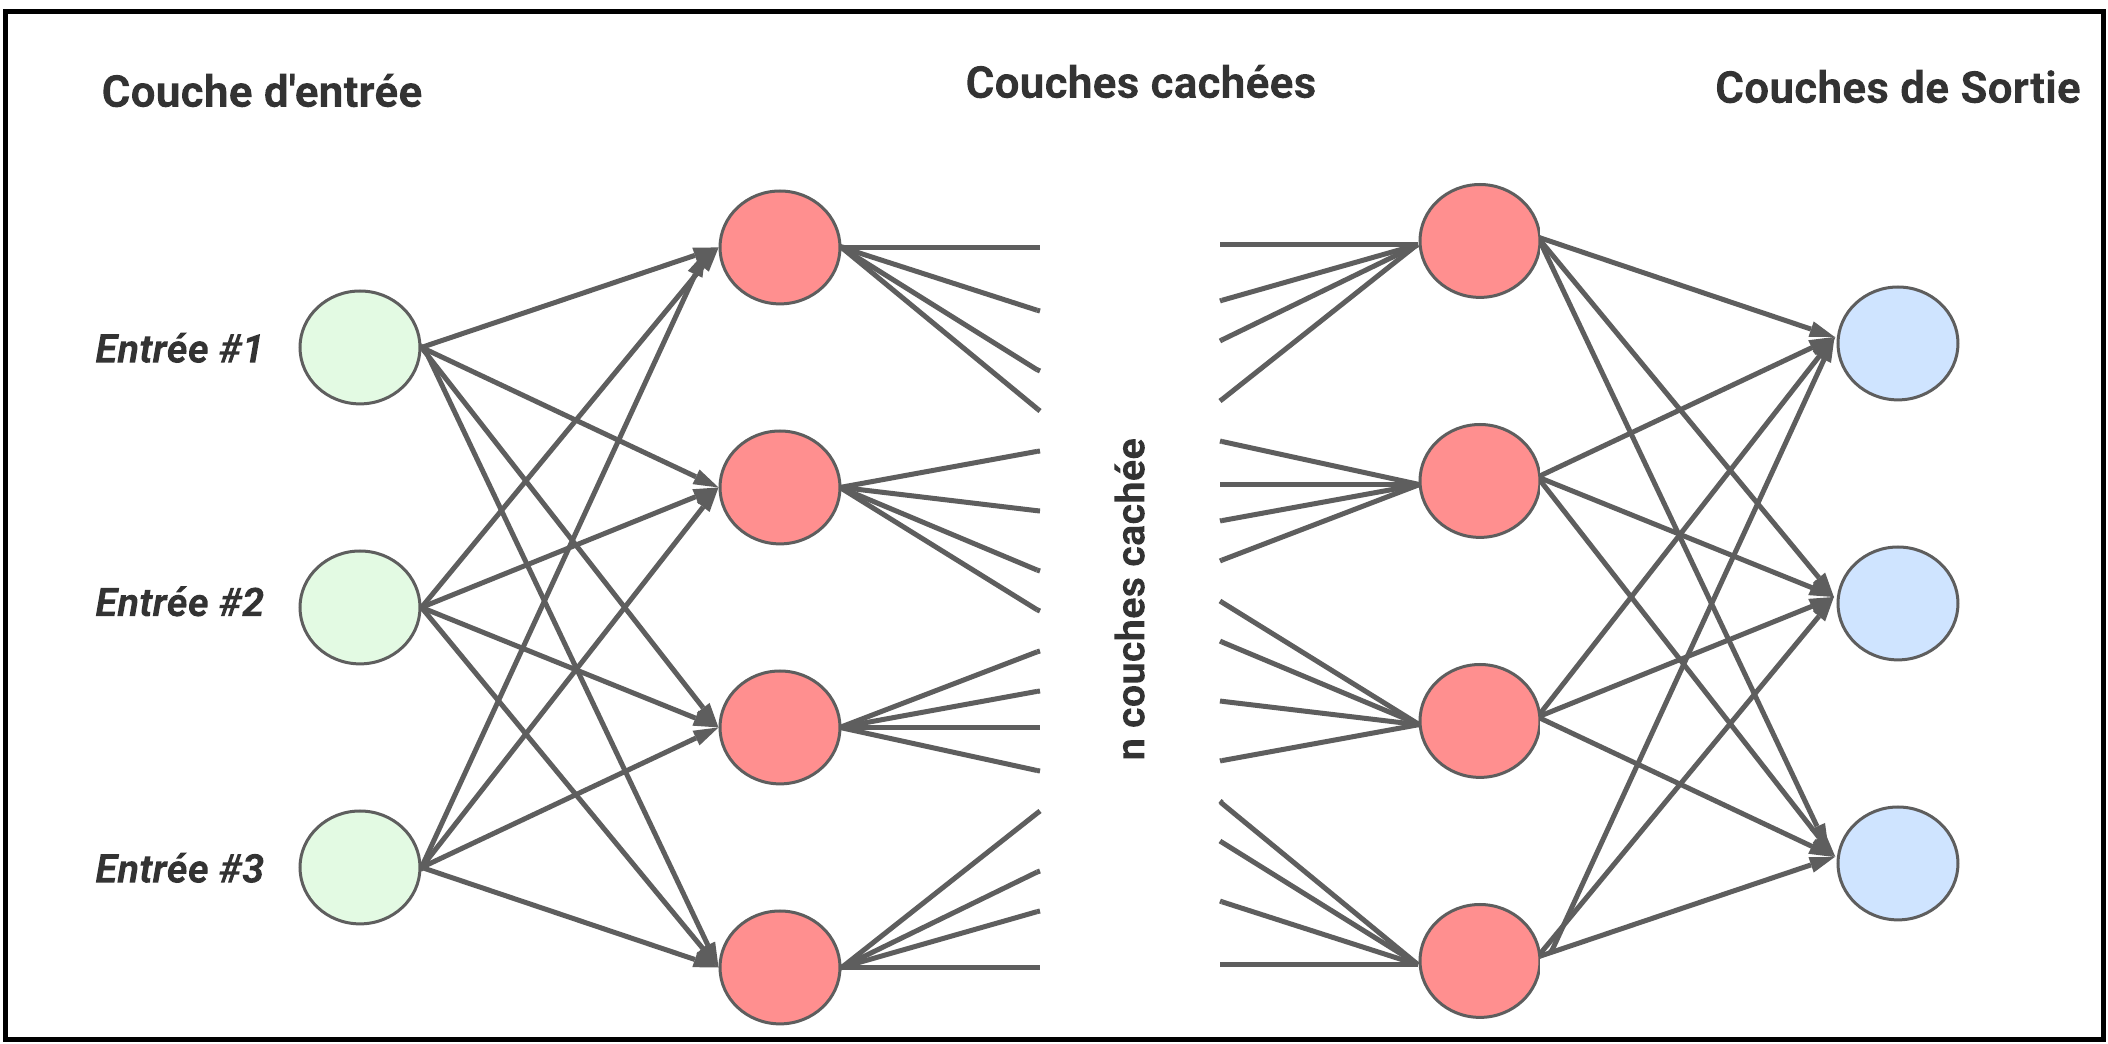
\includegraphics[width=\textwidth]{Figure 2.5.png}
  \caption{Principe du Deep Learning  }
  \label{fig:Principe du Deep Learning  }
\end{figure}

Figure 2.6 présente comment l’apprentissage profond a tendance à bien fonctionner avec de grandes quantités de données, tandis que les modèles d’apprentissage automatique plus traditionnels cessent de s’améliorer à un moment donné.
\clearpage
La performance des réseaux de neurones s'est largement améliorée lorsque les capacités de calcul ont augmenté. Cela a permis d'augmenter le nombre de couches cachées (d'où le nom de deep learning) pour des calculs en un temps acceptable.(Figure 26 \footnote{\shortcite{alom2019state}})
\begin{figure}[!h]
  \centering
  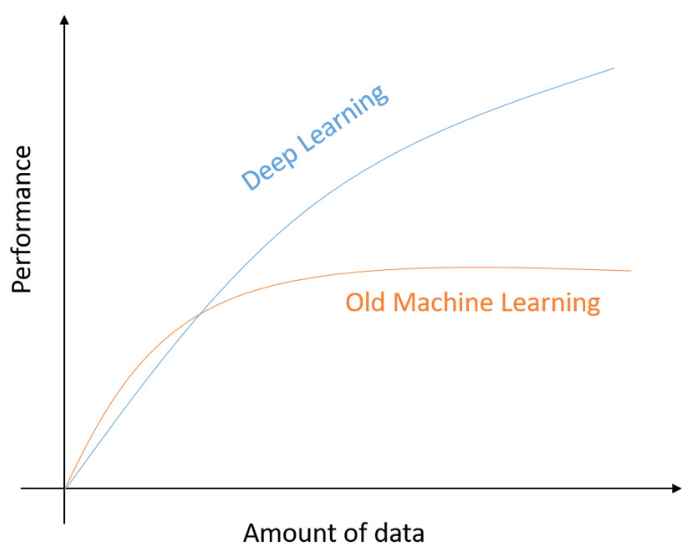
\includegraphics[width=12cm,height=10cm]{Figure 2.6.png}
  \caption{Performance du Deep Learning vs les modèles traditionnels selon la quantité des données.}
  \label{fig:Deep Learning vs les modèles traditionnels. }
\end{figure}
\newline
L'apprentissage profond englobe plusieurs types d'algorithmes, et l'un des plus utilisés est le réseau de neurones convolutifs (CNN en anglais).

\subsection{CNN}
En apprentissage profond, un CNN est une classe de réseaux neuronaux profonds, le plus souvent utilisée pour analyser des images visuelles.
 Lorsque nous pensons à un réseau neuronal, nous pensons à des multiplications de matrices, mais ce n'est pas le cas avec ConvNet. Il utilise une technique spéciale appelée convolution.\\En mathématiques, la convolution est une opération mathématique sur deux fonctions qui produit une troisième fonction qui exprime comment la forme de l'une est modifiée par l'autre.
 \begin{figure}[!h]
  \centering
  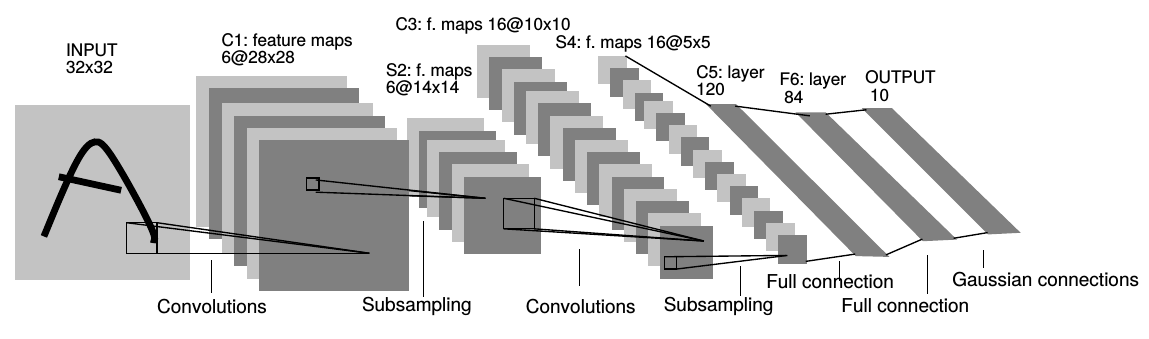
\includegraphics[width=\textwidth]{Figure 2.7.png}
  \caption{Gradient-Based appliqué à la reconnaissance de documents}
  \label{fig:Gradient-Based appliqué à la reconnaissance de docuemnts. }
\end{figure}

La figure 2.7 \footnote{\shortcite{lecun1998gradient}} montre l'architecture d'un réseau de neurones convolutif (ConvNet/CNN) utilisé pour la reconnaissance de caractères manuscrits.
La figure montre une succession de couches de traitement d'informations qui sont organisées de manière hiérarchique, permettant au modèle de capturer des caractéristiques de plus en plus abstraites de l'image en entrée.
\subsubsection{Couches}
Les CNN sont composés de différentes couches qui permettent d'extraire des informations de plus en plus complexes des images en entrée. Plus le nombre de couches est important, plus le modèle est complexe et capable de détecter des caractéristiques plus précises dans l'image.

\begin{itemize}
    \item [$\bullet$]\textbf{Couche de convolution (CONV)}:\\
    La première couche d'un CNN est généralement une couche de convolution, qui permet d'extraire les caractéristiques de l'image en appliquant des filtres sur les pixels de l'image. Cette opération permet de préserver la relation entre les différentes parties de l'image. En utilisant une taille de filtre plus petite que celle de l'image, la taille de l'image est réduite sans perdre la relation entre les pixels. Par exemple, en appliquant une convolution à une image de 5x5 avec un filtre de 3x3 et un pas de 1x1, l'image de sortie sera de 3x3 (soit une réduction de \%64 
    de la complexité de l'image).
    
\par Ces couches de convolution sont donc cruciales pour extraire des informations importantes des images en entrée et sont souvent suivies de couches de sous-échantillonnage (pooling) pour réduire la dimension de la sortie. L'empilement de ces couches permet de construire des modèles de plus en plus complexes et performants pour des tâches de reconnaissance d'images, de détection d'objets, et bien d'autres. (Figure 2.8 et 2.9 \footnote{\shortcite{mnist-image-classification}})
\clearpage
\begin{figure}[!h]
  \centering
  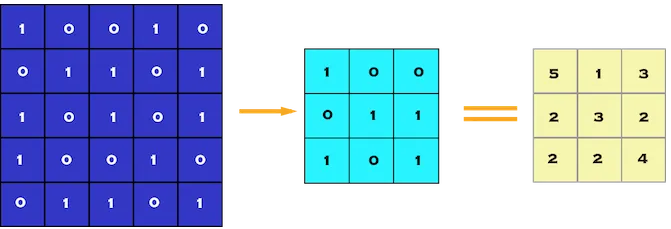
\includegraphics[width=\textwidth]{Figure 2.8.png}
  \caption{Convolution d'une image de 5 x 5 pixels avec un filtre de 3 x 3 pixels (pas de 1 x 1 pixel) }
  \label{fig:CONV}
\end{figure}


 \vspace{0.5em}
    \item [$\bullet$]\textbf{Couche de Pooling  (POOL)}:\\
  La couche de Pooling est une opération généralement appliquée entre deux couches de convolution. Celle-ci reçoit en entrée les features maps formées en sortie de la couche de convolution et son rôle est de réduire la taille des images, tout en préservant leurs caractéristiques les plus essentielles. Parmi les plus utilisés, on retrouve le max-pooling mentionné précédemment ou encore l’average pooling dont l’opération consiste à conserver à chaque pas, la valeur moyenne de la fenêtre de filtre. 
Finalement, on obtient en sortie de cette couche de Pooling, le même nombre de feature maps qu’en entrée mais considérablement compressées
\begin{figure}[!h]
  \centering
  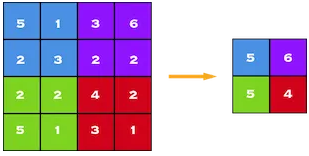
\includegraphics[width=10cm,height=5cm]{Figure 2.9 .png}
  \caption{Max pooling par un facteur de 2 x 2 }
  \label{fig:POOL}
\end{figure}

\newpage
    \item [$\bullet$]\textbf{Couche d’activation ReLU }:\\
  Cette couche remplace toutes les valeurs négatives reçues en entrées par des zéros. L’intérêt de ces couches d’activation est de rendre le modèle non linéaire et de ce fait plus complexe.\\
ReLU désigne la fonction réelle non-linéaire définie par 
$ReLU = max(0,x)$
\begin{figure}[!h]
  \centering
  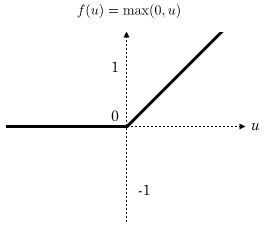
\includegraphics[width=10cm,height=8cm]{Figure 2.10.png}
  \caption{Allure de la fonction ReLU }
  \label{fig:Allure de la fonction ReLU}
\end{figure}

\vspace{0.5em}
    \item [$\bullet$]\textbf{Couche Fully Connected (FC)}:\\
Ces couches sont placées en fin d’architecture de CNN et sont entièrement connectées à tous les neurones de sorties (d’où le terme fully-connected). Après avoir reçu un vecteur en entrée, la couche FC applique successivement une combinaison linéaire puis une fonction d’activation dans le but final de classifier l’input image (voir figure 2.5). Elle renvoie enfin en sortie un vecteur de taille d correspondant au nombre de classes dans lequel chaque composante représente la probabilité pour l’input image d’appartenir à une classe.

\vspace{0.5em}
    \item [$\bullet$]\textbf{Couche de normalisation de lot}:\\
Cette couche normalise les activations des couches précédentes pour accélérer l'apprentissage et améliorer la généralisation.
\vspace{0.5em}
    \item [$\bullet$]\textbf{Couche de dropout }:\\
Cette couche désactive de manière aléatoire certains neurones pendant l'entraînement pour éviter le sur-apprentissage et améliorer la généralisation.
\end{itemize}
\vspace{0.5cm}
Ces couches peuvent être combinées de différentes manières pour construire des architectures de CNN complexes qui sont capables de résoudre une grande variété de tâches de vision par ordinateur.

\subsubsection{Optimiseurs}
Les optimiseurs sont des algorithmes utilisés pour ajuster les poids de chaque couche du réseau de neurones convolutif pendant l'entraînement afin de minimiser la fonction de perte.
La fonction de perte mesure la différence entre les valeurs prédites par le modèle et les vraies valeurs. L'objectif est de minimiser cette différence pour que les prédictions soient aussi précises que possible. Les optimiseurs tels que l'algorithme de descente de gradient stochastique (SGD) ou l'algorithme d'Adam ajustent les poids des couches du réseau de neurones convolutif pour minimiser la fonction de perte.

\section{Paramètres et hyperparamètres du ML et du DL}
Dans ML/DL, les modèles sont définis ou représentés par des paramètres de modèle. Cependant, le processus d’entrainement d'un modèle implique de choisir les meilleurs hyperparamètres. Ceci est utilisé par les algorithmes d'apprentissage pour apprendre les meilleurs paramètres qui mappent correctement les caractéristiques d'entrée aux étiquettes ou aux cibles pour obtenir une certaine forme d'intelligence.
\subsection{Paramètres}
Les paramètres sont internes au modèle. Autrement dit, ils sont appris ou déduits uniquement à partir des données pendant l’entrainement, car l'algorithme utilisé tente d'apprendre les associations entre les caractéristiques d'entrée et les étiquettes ou les cibles. L’entrainement du modèle commence généralement par l'initialisation des paramètres à une certaine valeur (aléatoire ou définie sur zéro). \\Au fur et à mesure de l'apprentissage, les valeurs initiales sont mises à jour à l'aide d'un algorithme d'optimisation (comme gradient descent). Un algorithme d'apprentissage met à jour en permanence les valeurs des paramètres au fur et à mesure qu'il s'entraîne, mais ne modifie pas les valeurs des hyperparamètres définies par le concepteur du modèle. 

A la fin du processus d'apprentissage, les paramètres du modèle constituent le modèle lui-même.
Voici quelques exemples courants :
\begin{itemize}
    \item Les coefficients (ou weights) des modèles de régression linéaire et logistique.
    \item Cluster centroïdes en clustering.
\end{itemize}

Les paramètres de ML/DL sont des valeurs qui peuvent être modifiées et ils sont influencées par le choix des hyperparamètres à fournir. Ainsi, si vous définissez les hyperparamètres avant le début de l'entraînement, l'algorithme d'apprentissage les utilisera pour apprendre les paramètres. 

\subsection{Hyperparamètres}
Dans le ML/DL, un hyperparamètre est tout ce dont la valeur ou la configuration est choisie avant le début de l’entraînement et dont la valeur ou la configuration ne change pas à la fin de la formation. 

Voici quelques exemples courants :
\begin{itemize}
    \item Train-test split ratio.
    \item Nombre de couches cachées.
    \item Nombré d'époques.
    \item Taille du lot.
\end{itemize}

\subsubsection{Taille du lot(Batch size)}
Batch Size est un hyperparamètre qui définit le nombre d'échantillons à traiter avant de mettre à jour les paramètres du modèle interne. Utilisons l'approche la plus simple et comparons les performances des modèles où seule Batch Size varie. (Figure 2.11 \footnote{\shortcite{batchsize_medium}})

\begin{itemize}
    \item Courbe orangée: Batch Size: 64
    \item Courbe bleue: Batch Size: 256
    \item Courbe violette: Batch Size: 1024
\end{itemize}
L'axe des abscisses montre le nombre d'époques d'entraînement, et l'axe des ordonnées est étiqueté pour chaque graphique. Nous observons une tendance claire entre la taille de lot et la précision asymptotique de l'ensemble de test (et d'entraînement). Nous en tirons une conclusion :$\rightarrow$ La taille du lot \textbf{augmente}, la précision du test \textbf{diminue}. 
\clearpage
\begin{figure}[!h]
  \centering
  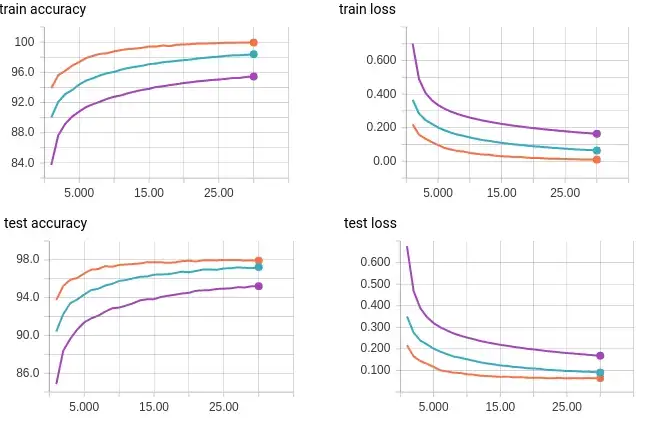
\includegraphics[width=12 cm,height=10cm]{Figure 2.11.png}
  \caption{Précision et perte lors de la variation du Batch Size  }
  \label{fig:Batch Size}
\end{figure}


\subsubsection{Époques}
Dans l'apprentissage automatique, une époque est une passe complète d'un ensemble de données d'entraînement à travers un réseau de neurones. En d'autres termes, l'algorithme d'apprentissage examine tous les exemples d'entraînement une fois. Les époques sont donc une mesure de l'itération de l'ensemble des données d'entraînement. En règle générale, plus le nombre d’époques est élevé, plus le modèle est entraîné. Cependant, il est important de noter que l'augmentation du nombre d’époques n'entraîne pas toujours une amélioration des performances du modèle. En effet, l'overfitting peut se produire si le modèle est trop entraîné sur les données d'entraînement. (Figure 2.12\footnote{\shortcite{deepai_epoch}}). Par conséquent, il est important de déterminer le nombre optimal d’époques pour entraîner le modèle. Cela peut être fait en utilisant des techniques d'optimisation d'hyperparamètres telles que la recherche par grille, la recherche aléatoire ou la recherche bayé-sienne.
\clearpage
\begin{figure}[!h]
  \centering
  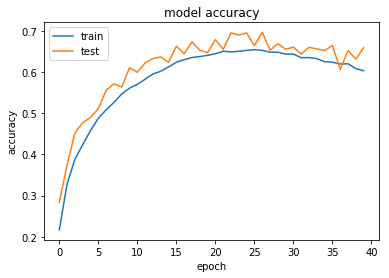
\includegraphics[width=12 cm,height=8cm]{Figure 2.12.png}
  \caption{La précision d’un modèle en fonction de nombre d’époques}
  \label{fig:Epoque}
\end{figure}

\vspace{1cm}

\begin{itemize}
    \item [$\bullet$]\textbf{La recherche par grille}:\\
    Cette méthode a été introduite dans le domaine de l'optimisation des hyperparamètres dans les années 1960 par un statisticien américain du nom de Marvin Zelen.\\
Elle consisterait à tester différents nombres d'époques pour entraîner le modèle. Les performances du modèle seraient évaluées pour chaque combinaison d'hyperparamètres en utilisant une métrique d'évaluation telle que la précision (accuracy) ou la perte (loss).\\
Cependant, la recherche par grille peut être coûteuse en termes de temps et de ressources, surtout lorsque le nombre d'hyperparamètres et de valeurs à tester est élevé. 

\vspace{1cm}
\item [$\bullet$]\textbf{La recherche bayésienne }:\\
Cette méthode est une méthode d'optimisation des hyperparamètres qui permet de trouver les valeurs optimales pour les hyperparamètres d'un modèle en utilisant une approche probabiliste. Cette méthode a été introduite dans un article de 1997 intitulé "Bayesian optimization for machine learning" par David J.C. MacKay.\\
Depuis lors, la recherche bayésienne est devenue une méthode populaire pour l'optimisation des hyperparamètres dans le domaine de l'apprentissage automatique. Elle est couramment utilisée pour trouver les valeurs optimales pour des hyperparamètres tels que le taux d'apprentissage, le nombre de couches cachées, la taille du lot, etc.\\
 Cette méthode présente également certains points négatifs. Tout d'abord, elle nécessite un temps de calcul plus important que la recherche par grille car elle doit effectuer plusieurs évaluations de modèle. De plus, elle nécessite de spécifier une distribution de probabilité initiale sur les hyperparamètres, ce qui peut être difficile à faire dans certains cas. Enfin, la méthode est sensible aux choix d'hyperparamètres initiaux et de la fonction d'acquisition utilisée pour sélectionner les prochaines valeurs d'hyperparamètres à évaluer.
\end{itemize}
\vspace{1.25cm}
\section{Conclusion}
En conclusion, le DL, et en particulier CNN, ont apporté des avancées majeures dans le domaine de l'apprentissage automatique pour l'analyse d'images et de vidéos. Les hyperparamètres, tels que le nombre d'époques, jouent un rôle crucial dans la performance de ces modèles.\\
Cependant, l'estimation du nombre optimal d'époques reste un défi important pour les praticiens de l'apprentissage automatique. C'est pourquoi de nouvelles techniques sont nécessaires pour déterminer le nombre d'époques optimal de manière plus précise et plus efficace.\\
Dans ce chapitre, nous avons exploré l'état de l'art des hyperparamètres, en nous concentrant sur les époques, et avons discuté de l'importance de l'optimisation de ces paramètres pour améliorer les performances des modèles.\\
Nous avons également ouvert la porte à de nouvelles approches pour déterminer le nombre optimal d'époques, en utilisant des techniques d'estimation de densité de probabilité non paramétriques pour développer une nouvelle métrique d'évaluation.\\
Cette nouvelle approche pourrait offrir de nouvelles perspectives pour optimiser les modèles CNN et améliorer leurs performances. Il reste cependant du travail à faire pour développer et valider cette approche, mais elle pourrait contribuer à une meilleure compréhension des hyperparamètres et à une amélioration significative de la performance des modèles.

\clearpage

\thispagestyle{empty}


\begin{tikzpicture}[remember picture,overlay]
  \begin{scope}[on background layer]
    \fill[white,opacity=.8] (current page.north west) rectangle (current page.south east);
  \end{scope}
\end{tikzpicture}

\vspace{3cm}

\begin{center}
\vspace{6cm}
\textit{\large "Les simulations permettent de faire des erreurs à moindre coût."} \\- Andrew Ng
\end{center}

\clearpage % Ajout de la commande pour réinitialiser la numérotation des pages

\clearpage

\chapter{Simulations}
\section{Introduction}
Dans ce chapitre, nous allons explorer les performances des méthodes d'estimation de la ddp non paramétriques en utilisant des données simulées à partir de lois usuelles telles que la loi normale, la loi exponentielle et la loi uniforme. L'objectif de cette simulation est d'évaluer les performances de différentes méthodes d'estimation de la ddp et de comparer les résultats avec les vraies valeurs de la ddp.
Nous allons d'abord présenter les lois usuelles que nous allons simuler, notamment la loi normale et la loi exponentielle. Nous allons ensuite expliquer comment nous avons simulé ces lois à partir de données aléatoires. Nous allons ensuite utiliser des méthodes d'estimation de la ddp non paramétriques pour estimer la ddp des données simulées. Nous allons évaluer les performances de ces méthodes en utilisant EQM et les comparer avec les vraies valeurs de la ddp.
Cette simulation est importante car elle permettra de déterminer la performance des différentes méthodes d'estimation de la ddp non paramétriques dans des situations contrôlées. Les résultats de cette simulation pourront ensuite être généralisés à des situations plus complexes et réelles. Cette simulation est également importante car elle peut aider à comprendre les avantages et les limites des différentes méthodes d'estimation de la ddp non paramétriques. Ces informations peuvent être utiles pour choisir la méthode la plus appropriée dans différentes situations d'analyse de données.
En conclusion, ce chapitre de simulation permettra d'évaluer les performances des méthodes d'estimation de la ddp non paramétriques à partir de données simulées. Nous espérons que les résultats de cette simulation pourront fournir des informations utiles sur les performances des différentes méthodes d'estimation de la ddp et aider à choisir la méthode la plus appropriée dans différentes situations d'analyse de données.
\newpage

\section{Description des lois utilisées}
Nous avons procédé à des simulations sur différentes lois de probabilité, à savoir:
\newline 
\newline    
\begin{itemize}
   \item[$\bullet$] Une densité de probabilité, en l'occurrence une \textbf{loi normale}.\\
   \begin{lstlisting}
    import numpy as np
    #m Moyenne
    #s ecart-type
    #n taille echantillon
def generation_LN(m, s, n):
    mln = np.zeros(n)
    LN = np.random.randn(n)
    for i in range(n):
        LN[i] = m + s * LN[i]
    return(LN)

    \end{lstlisting}

    \vspace{1.5cm}
       \item[$\bullet$] Une densité de probabilité mixte(combinée), en l'occurrence une \textbf{loi exponentielle} et une \textbf{loi normale}.\\
   \begin{lstlisting}
    def generation_Mix(lam,mu,sigma,n_samples):
    #m Moyenne
    #sigma Ecart-type
    #lam Lambda
    #n_samples Taille echantillon
    samples = np.zeros(n_samples)
    for i in range(n_samples):
        if np.random.uniform() < lam:
            samples[i] = np.random.exponential(scale=1/lam)
        else:
            samples[i] = np.random.normal(loc=mu, scale=sigma)
            
    return(samples) 
    \end{lstlisting}

           \item[$\bullet$] Une densité de probabilité, en l'occurrence une \textbf{loi uniforme},\\ à savoir une loi uniforme entre $] a ,b [$.\\
           
   \begin{lstlisting}
    import numpy as np
def generation_LE(a,b,n):

    LE = np.random.uniform(low=a, high=b, size=n)

    return(LE)

    \end{lstlisting}
    \vspace{0.5cm}
\end{itemize}

Durant ces simulations nous comparer les performances des méthodes de noyau et de l’histogramme. Pour la méthode de noyau nous allons également comparer les performances en faisant varier les méthodes d’optimisation du paramètre de lissage.
\vspace{0.25cm}
\begin{itemize}
   \item[$\bullet$]\textbf{Histogramme} :\\
   Les étapes comprennent la division de l'intervalle des données en bins (classes), le calcul de la fréquence dans chaque bin, et la normalisation des fréquences pour obtenir une estimation graphique de la ddp de l'échantillon de données.
En ce qui concerne l’optimisation de $h_N$ nous allons suivre cette méthode \shortcite{freedman1981histogram} :
$$
\begin{aligned}
n_{\text{I}} &= \left\lfloor n^{1/3} \right\rfloor \\
h_N &= \frac{a-b}{n_{\text{I}}} \\
\text{avec } \text{A} &= \{a_1, a_2, \ldots, a_n\} \\
a &= \max\{a_1, a_2, \ldots, a_n\} \\
b &= \min\{a_1, a_2, \ldots, a_n\} \\
\left\lfloor x \right\rfloor &= \max\{n \in \mathbb{Z} \mid n \leq x\}
\end{aligned}
$$
 \item[$\bullet$]\textbf{Noyau - ROT} :\\Cette méthode est prédéfinie en Python 3, donc va appeler la méthode adéquate directement. 
 \item[$\bullet$]\textbf{Noyau - LSCV} :\\Cette méthode utilise l’estimateur à noyau avec recherche du pas optimal en utilisant la classe GridSearchCV de la bibliothèque scikit-learn.  
 \item[$\bullet$]\textbf{Noyau - PlugIn} :\\Cette méthode utilise l’estimateur à noyau avec recherche du pas optimal en l’algorithme Plug-In 

   
\end{itemize}
\newpage
Comme métrique d’évaluation de performance, Nous avons opté pour EQM, c’est une mesure couramment utilisée pour évaluer la qualité d'une méthode d’estimation de probabilité, en calculant la moyenne des carrés des différences entre les densités estimées par la méthode concernée et les densités réelles.
\begin{equation}
    EQM = \frac{1}{n} \sum_{i=1}^n (f_i - \hat{f}_i)^2
\end{equation}
\myequations{Equation \ref{eq:Eq10}}
où :
\begin{itemize}
    \item $n$ est la taille de l'échantillon,
    \item $f$ est la densité réelle,
    \item $\hat{f}$ est la densité estimée.
\end{itemize}

\section{Simulation}
Nous allons tester les différentes méthodes sur quatre distributions G1, G2, G3, G4 et G5 \\ tel que :
\newline
\begin{itemize}
 \setlength\itemsep{12pt}
    \item[$\bullet$]\textbf{G1} représente une distribution uni-modale d’une \textbf{loi normale} :
    \begin{itemize}
    \item $m = 0.5$
    \item $\sigma = 0.1$
    \end{itemize}

    \item[$\bullet$]\textbf{G2} représente une distribution bimodale d’une \textbf{loi normale} :
    \begin{itemize}
    \item $m_1 = -0.5\qquad ; \qquad m_2 = 0.0$
    \item $\sigma_1 = 0.1 \qquad ; \qquad \sigma_2 = 0.1$
    \end{itemize}


        \item[$\bullet$]\textbf{G3} représente une distribution tri-modale d’une \textbf{loi normale} :
    \begin{itemize}
    \item $m_1 = -0.5\qquad ; \qquad m_2 = 0.0 \qquad ; \qquad m_3 = 0.4$
    \item $\sigma_1 = 0.1 \qquad ; \qquad \sigma_2 = 0.1 \qquad ; \qquad \sigma_3 = 0.1 $
    \end{itemize}


        \item[$\bullet$]\textbf{G4} représente un mélange bimodal d’une \textbf{loi normale} et une \textbf{loi exponentielle} :
    \begin{itemize}
    \item $m = 0$
    \item $\sigma = 0$
    \item $\lambda = 0.5$
    \end{itemize}

         \item[$\bullet$]\textbf{G5} représente une distribution uni-modale d’une \textbf{loi uniforme} rectangulaire :
    \begin{itemize}
    \item $a = 0$
    \item $b = 10$
    \end{itemize}

\end{itemize}

\newpage
Les tableaux suivants présentent respectivement les différentes valeurs de EQM de différentes distributions expérimentées selon la taille et le type d´échantillon.
\vspace{1cm}
\begin{table}[htbp]
  \centering
  
  \setlength{\extrarowheight}{6pt}
    \begin{tabular}{@{}lS[table-format=2.2e-1]S[table-format=1.2e-1]S[table-format=1.2e-1]S[table-format=1.2e-1]@{}}
    \toprule
     & \multicolumn{4}{c}{Taille} \\
     \cmidrule{2-5}
    Distribution & {500} & {750} & {1000} & {1500} \\
    \midrule
    G1    & 17.8e-3 & 2.7e-3 & 1.6e-3 & 1.95e-3 \\
    G2    & 16.3e-3 & 6.1e-3 & 2.5e-3 & 1.69e-3 \\
    G3    & 3.5e-3 & 3.1e-3 & 1.5e-3 & 0.6e-3 \\
    G4    & 0.26e-3 & 0.15e-3 & 0.04e-3 & 0.08e-3 \\
    G5    & 0.12e-3 & 0.1e-3 & 0.1e-3 & 0.1e-3 \\
    \bottomrule
    \end{tabular}%
    \caption{EQM - Noyau Plug-in }
  \label{tab:EQM - Noyau Plug-in}%
\end{table}%
\vspace{4cm}

\begin{table}[htbp]
  \centering
    \setlength{\extrarowheight}{6pt}
    \begin{tabular}{@{}lS[table-format=3.2e-1]S[table-format=3.2e-1]S[table-format=3.2e-1]S[table-format=3.2e-1]@{}}
    \toprule
     & \multicolumn{4}{c}{Taille} \\
     \cmidrule{2-5}
    Distribution & {500} & {750} & {1000} & {1500} \\
    \midrule
    G1    & 189e-3 & 132e-3 & 177e-3 & 161e-3 \\
    G2    & 74e-3 & 53e-3 & 45e-3 & 56e-3 \\
    G3    & 31e-3 & 30e-3 & 26e-3 & 24e-3 \\
    G4    & 0.6e-3 & 0.2e-3 & 0.17e-3 & 0.3e-3 \\
    G5    & 0.15e-3 & 0.11e-3 & 0.16e-3 & 0.11e-3 \\
    \bottomrule
    \end{tabular}%
      \caption{EQM - Noyau LSCV}    
  \label{tab:EQM - Noyau LSCV}%
\end{table}%


\begin{table}[htbp]
  \centering
    \setlength{\extrarowheight}{6pt}
    \begin{tabular}{@{}lS[table-format=3.1e-1]S[table-format=3.1e-1]S[table-format=3.1e-1]S[table-format=3.1e-1]@{}}
    \toprule
     & \multicolumn{4}{c}{Taille} \\
     \cmidrule{2-5}
    Distribution & {500} & {750} & {1000} & {1500} \\
    \midrule
    G1    & 947e-3 & 678e-3 & 732e-3 & 534e-3 \\
    G2    & 573e-3 & 351e-3 & 370e-3 & 310e-3 \\
    G3    & 237e-3 & 196e-3 & 130e-3 & 179e-3 \\
    G4    & 5.4e-3 & 4.3e-3 & 5.1e-3 & 4.4e-3 \\
    G5    & 1.2e-3 & 0.8e-3 & 0.9e-3 & 0.79e-3 \\
    \bottomrule
    \end{tabular}%
    \caption{EQM - Histogramme}
  \label{tab:EQM - Histogramme}%
\end{table}%

\begin{table}[htbp]
  \centering
      \setlength{\extrarowheight}{6pt}

    \begin{tabular}{@{}lS[table-format=3.1e-1]S[table-format=3.1e-1]S[table-format=3.1e-1]S[table-format=3.1e-1]@{}}
    \toprule
    & \multicolumn{4}{c}{Taille} \\
    \cmidrule{2-5}
    Group & {500} & {750} & {1000} & {1500} \\
    \midrule
    G1 & 2170e-3 & 1908e-3 & 2060e-3 & 1786e-3 \\
    G2 & 645e-3 & 647e-3 & 615e-3 & 670e-3 \\
    G3 & 330e-3 & 419e-3 & 497e-3 & 325e-3 \\
    G4 & 7.5e-3 & 7.1e-3 & 7.6e-3 & 6.8e-3 \\
    G5 & 5e-3 & 5.1e-3 & 5e-3 & 5e-3 \\
    \bottomrule
    \end{tabular}%
    \caption{EQM - Noyau ROT}
  \label{tab:addlabel}%
\end{table}%

 Ci-dessous, nous allons représenter les ddp estimés pour une taille d'échantillon 1500 et pour les 5 distributions (G1$,..,$ G5). Nous avons choisi cette taille car plus l'échantillon est élevée meilleure est l'estimation. 

\begin{figure}[!h]
  \centering
  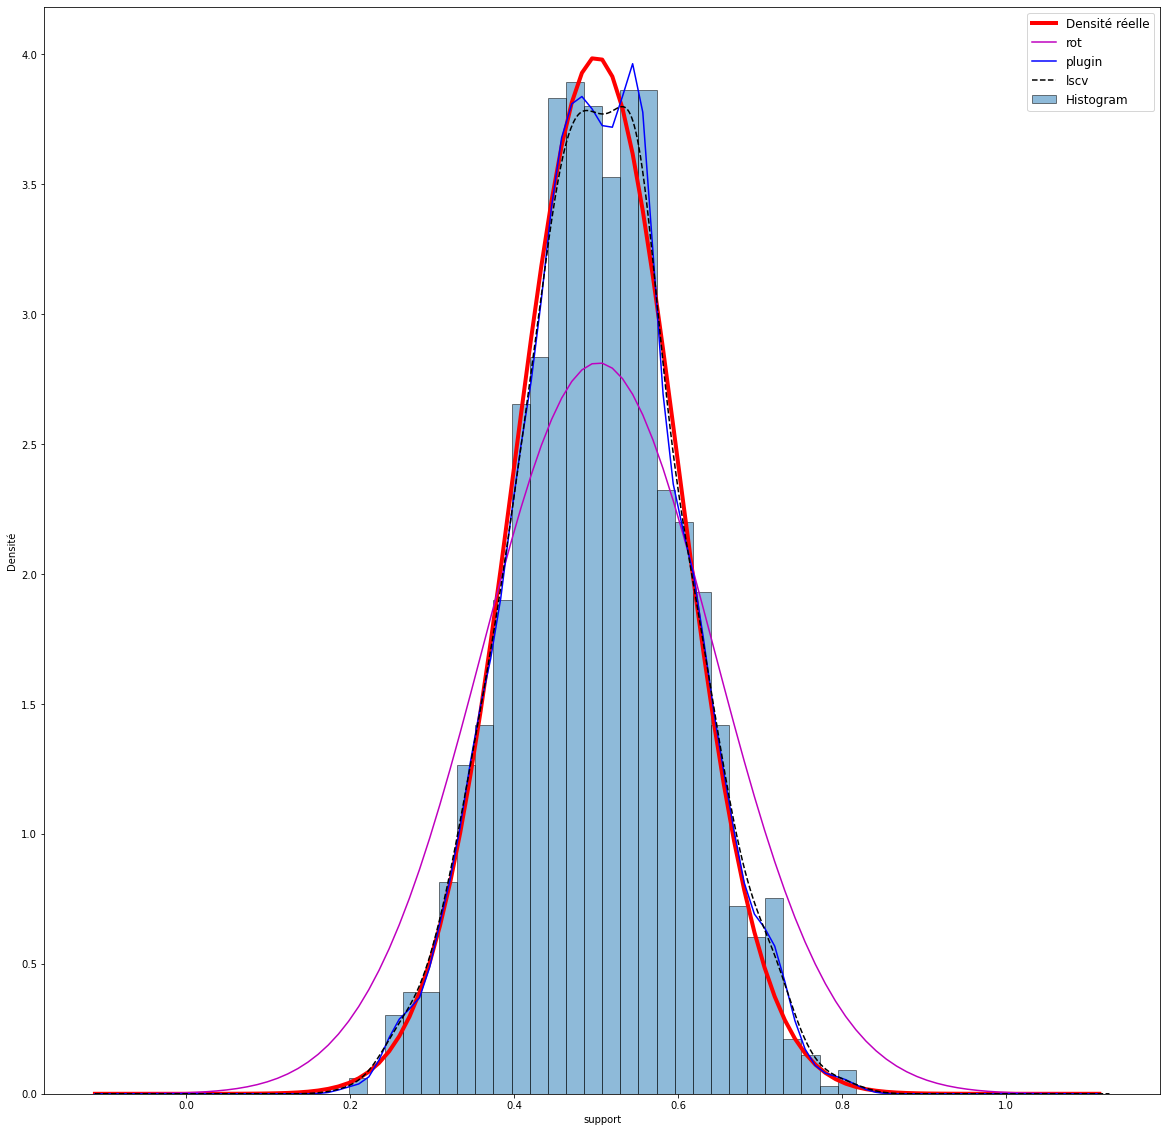
\includegraphics[width=\textwidth]{figure 3.1.png}
  \caption{Distribution G1}
  \label{fig:Différentes méthodes appliquées à la distribution G1}
\end{figure}
En observant la figure 3.1, nous pouvons constater que la méthode de l'histogramme présente des limitations en termes de précision de l'estimation de densité. Les rectangles utilisés pour représenter les classes de données introduisent des marges d'erreur, ce qui peut conduire à des estimations moins précises. Donc nous pouvons éliminer la méthode de l'histogramme dans la suite des simulations.
\clearpage
\begin{figure}[!h]
  \centering
  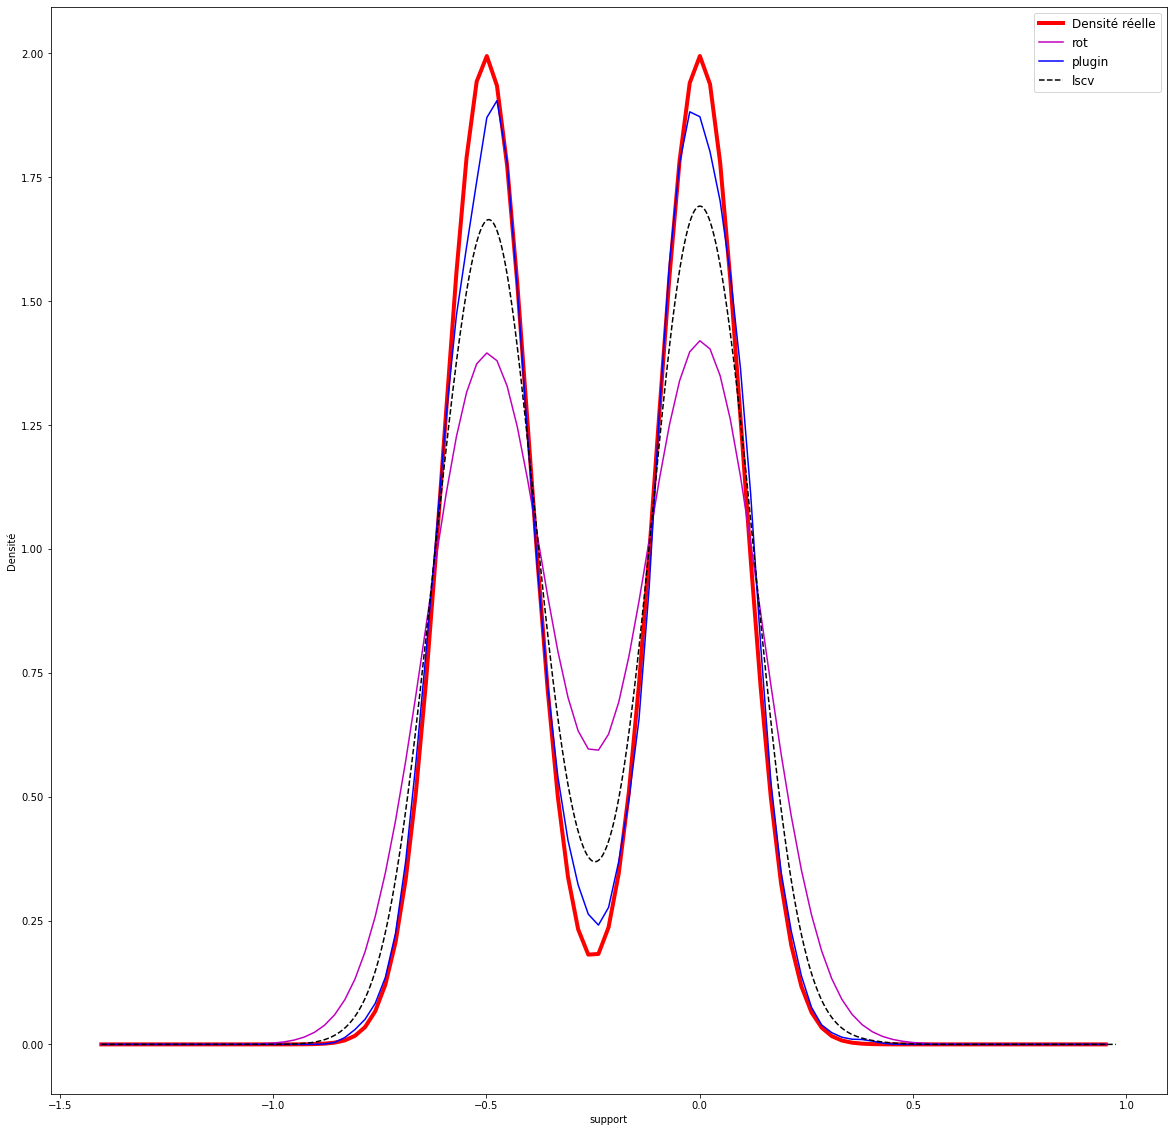
\includegraphics[width=\textwidth]{figure 3.2.png }
  \caption{Distribution G2}
  \label{fig:Différentes méthodes appliquées à la distribution G2}
\end{figure}
En examinant attentivement la figure 3.2, la méthode ROT semble produire des estimations moins précises par rapport aux méthodes LSCV  et PLUG-IN. Il est donc justifié d'éliminer la méthode ROT de nos simulations ultérieures et de poursuivre notre exploration avec les méthodes LSCV et PLUG-IN. 
\clearpage
\begin{figure}[!h]
  \centering
  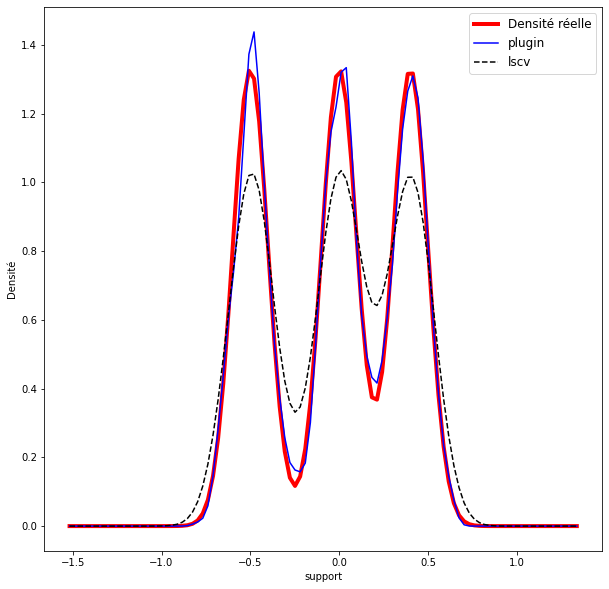
\includegraphics[width=\textwidth]{figure 3.3.png}
  \caption{Distribution G3}
  \label{fig:Différentes méthodes appliquées à la distribution G3}
\end{figure}
\clearpage
\begin{figure}[!h]
  \centering
  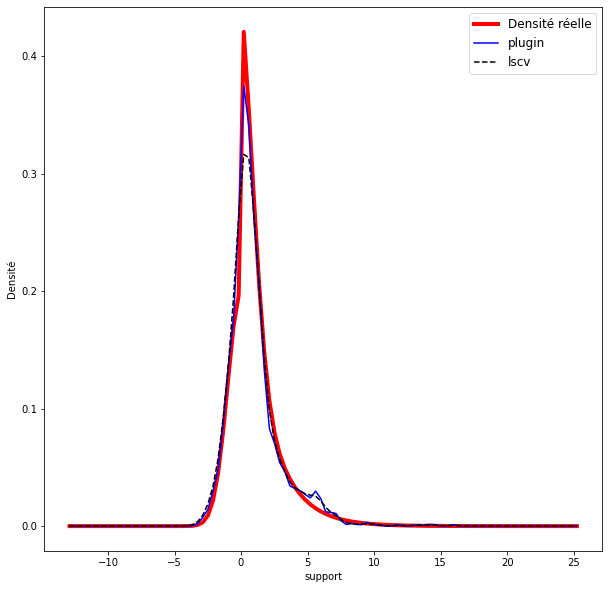
\includegraphics[width=\textwidth]{figure 3.4.png}
  \caption{Distribution G4}
  \label{fig:Différentes méthodes appliquées à la distribution G4}
\end{figure}
En analysant les deux figure 3.3 et 3.4, pour des distributions plus complexes, il devient évident que la méthode PLUG-IN produit des estimations plus précises que la méthode LSCV.
\clearpage
\begin{figure}[!h]
  \centering
  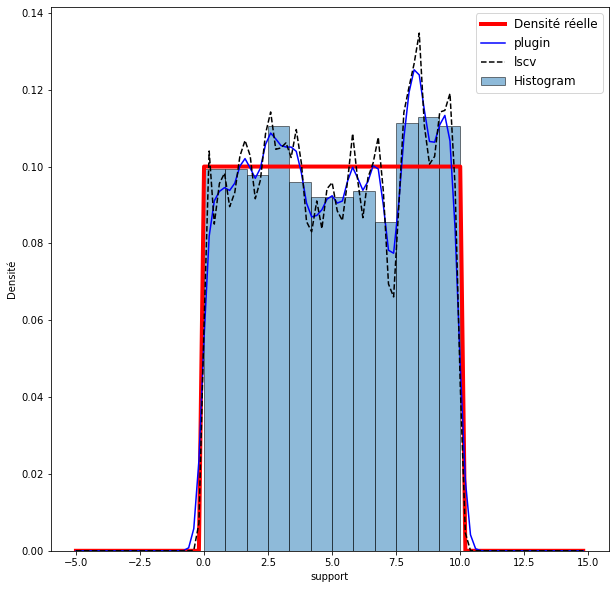
\includegraphics[width=\textwidth]{figure 3.5.png}
  \caption{Distribution G5}
  \label{fig:Différentes méthodes appliquées à la distribution G5}
\end{figure}
Lors de la simulation d'une loi uniforme (G5), nous avons remarqué que la méthode de l'histogramme peut fournir des estimations raisonnables de la densité. Les rectangles utilisés dans l'histogramme peuvent bien représenter la distribution uniforme, ce qui conduit à des estimations relativement précises. Cependant, en consultant les tables 3.1, 3.2, 3.3 et 3.4, nous avons remarqué que pour la distribution G5 avec un échantillon de taille 1500, la méthode PLUG-IN présente le plus faible EQM.

Les figures dans la page suivante présentent évolution EQM par taille d'échantillon pour différentes méthodes pour les 5 distributions (G1...G5) :  
\begin{figure}[!h]
  \centering
  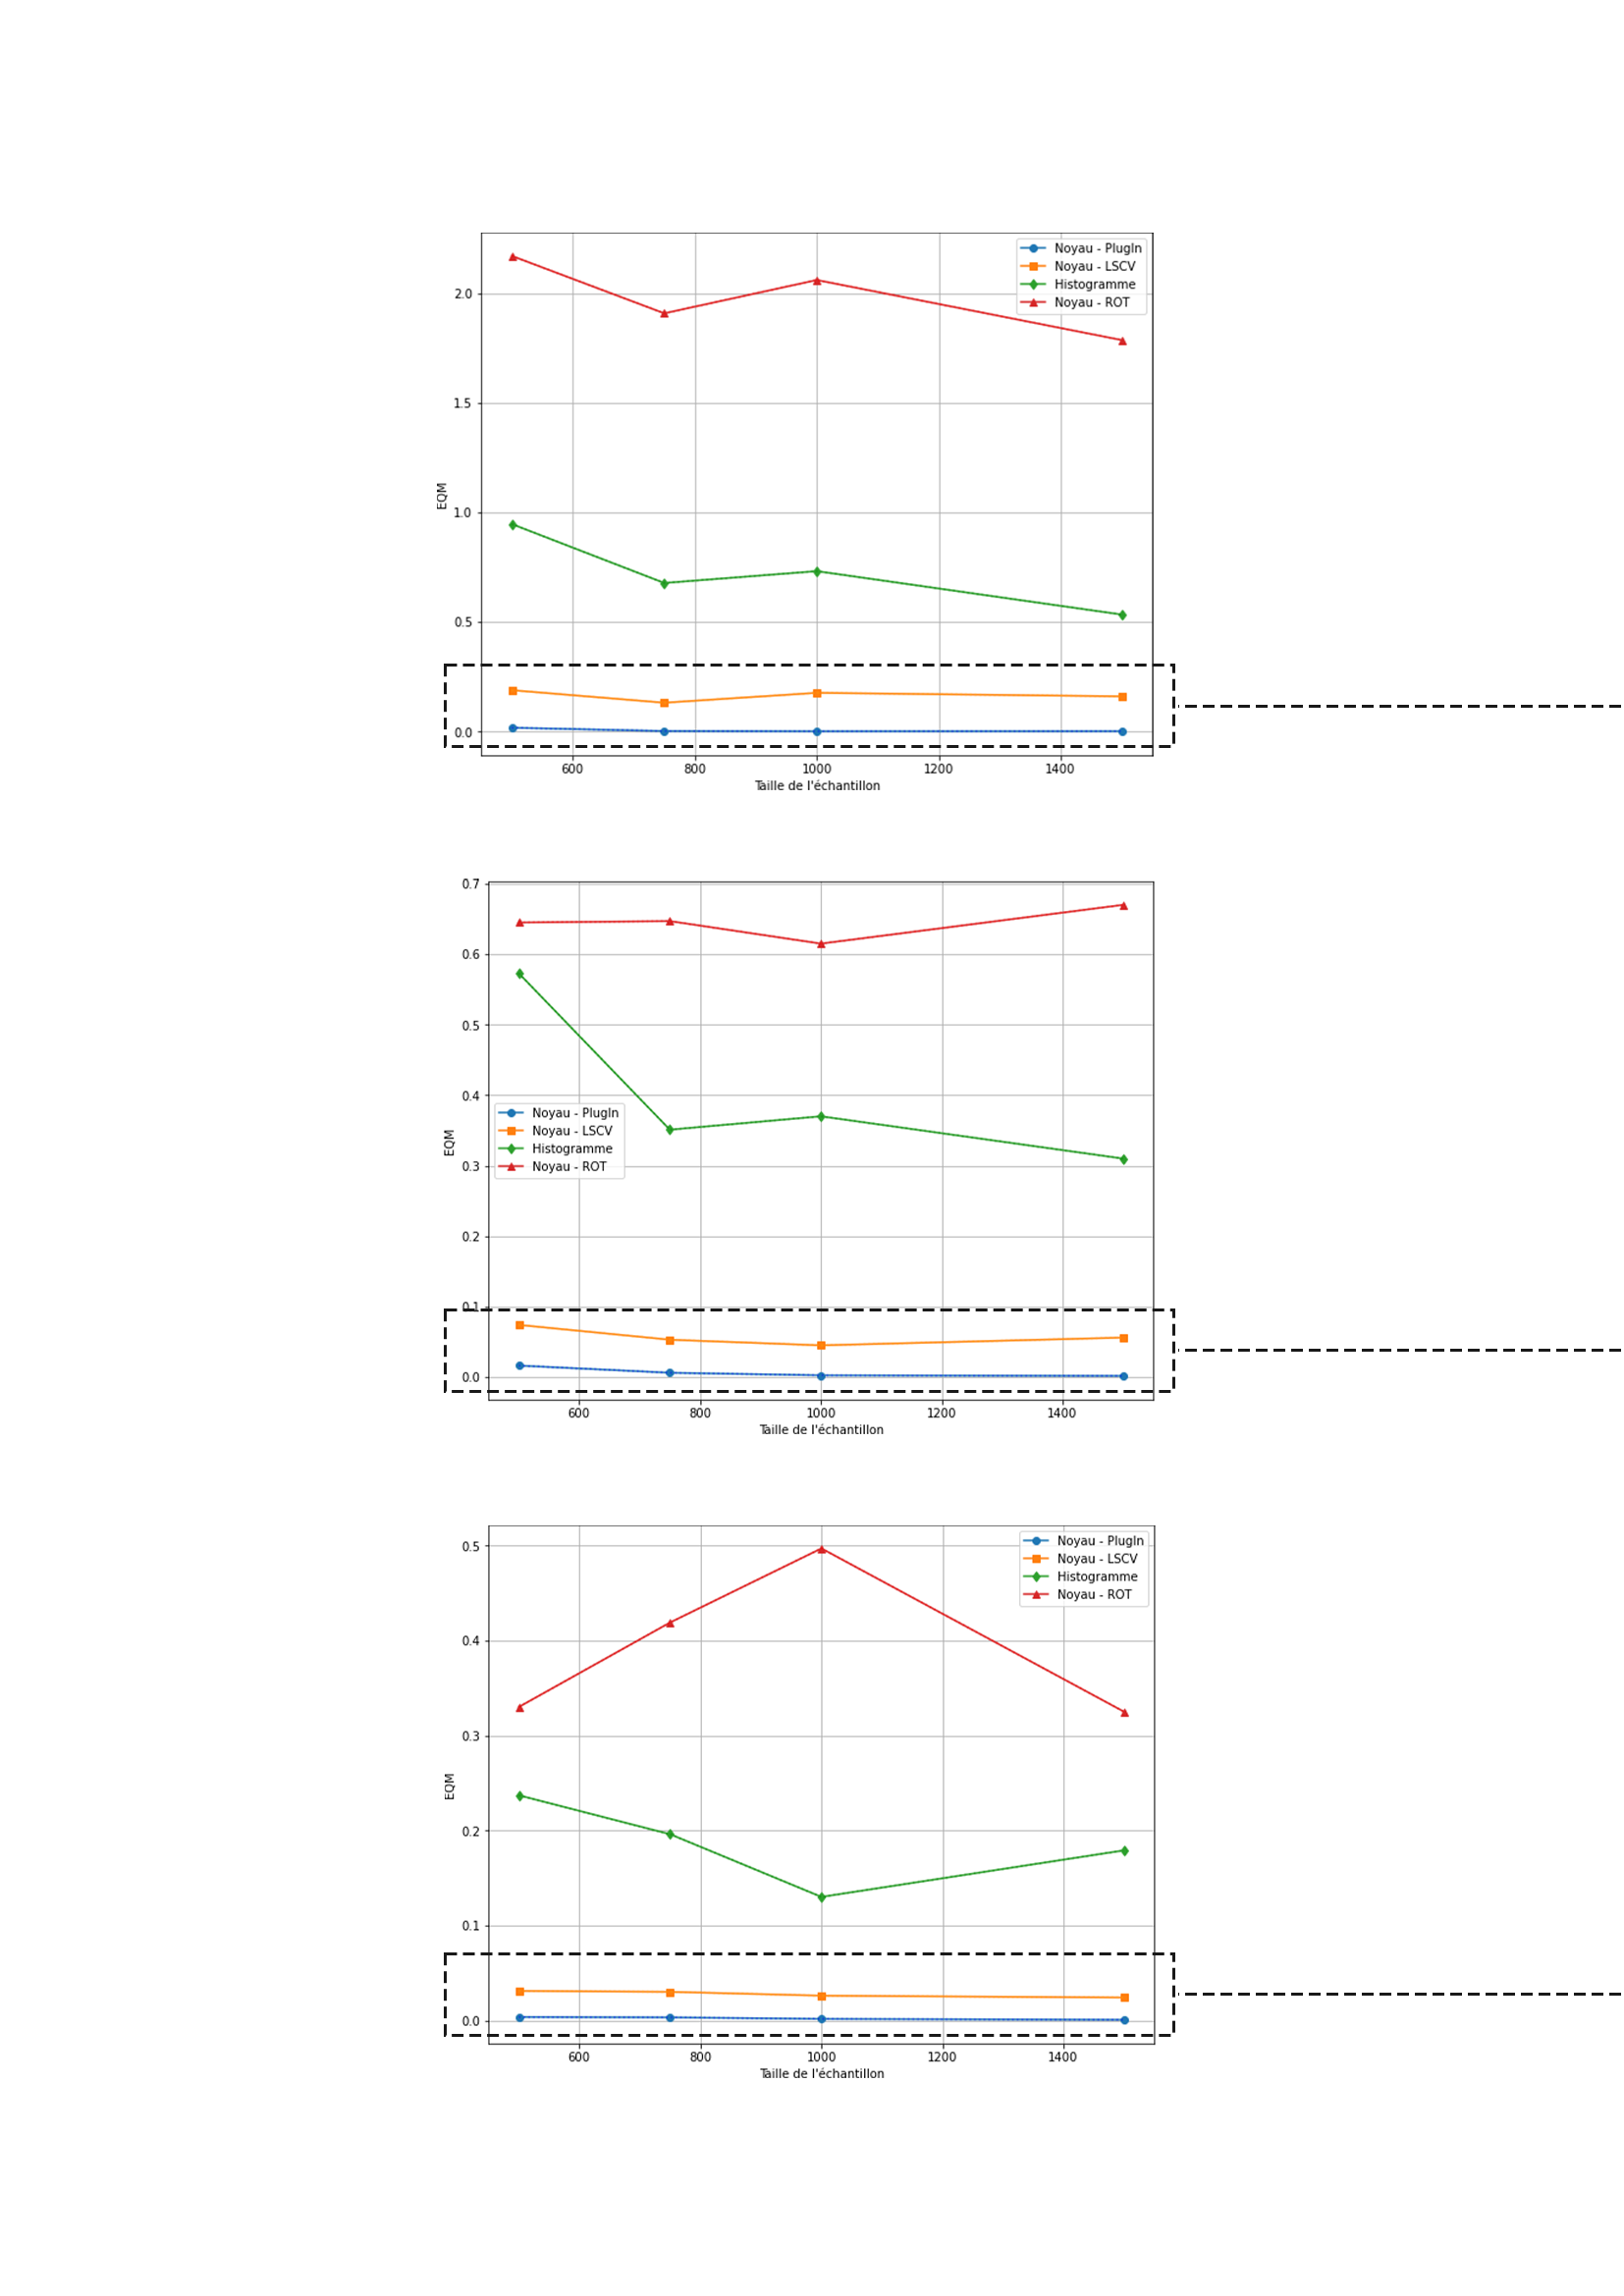
\includegraphics[width=\textwidth]{P 01.png}
  \caption{EQM : G1-G2-G3}
  \label{fig:G1-G2-G3}
\end{figure}
\begin{figure}[!h]
  \centering
  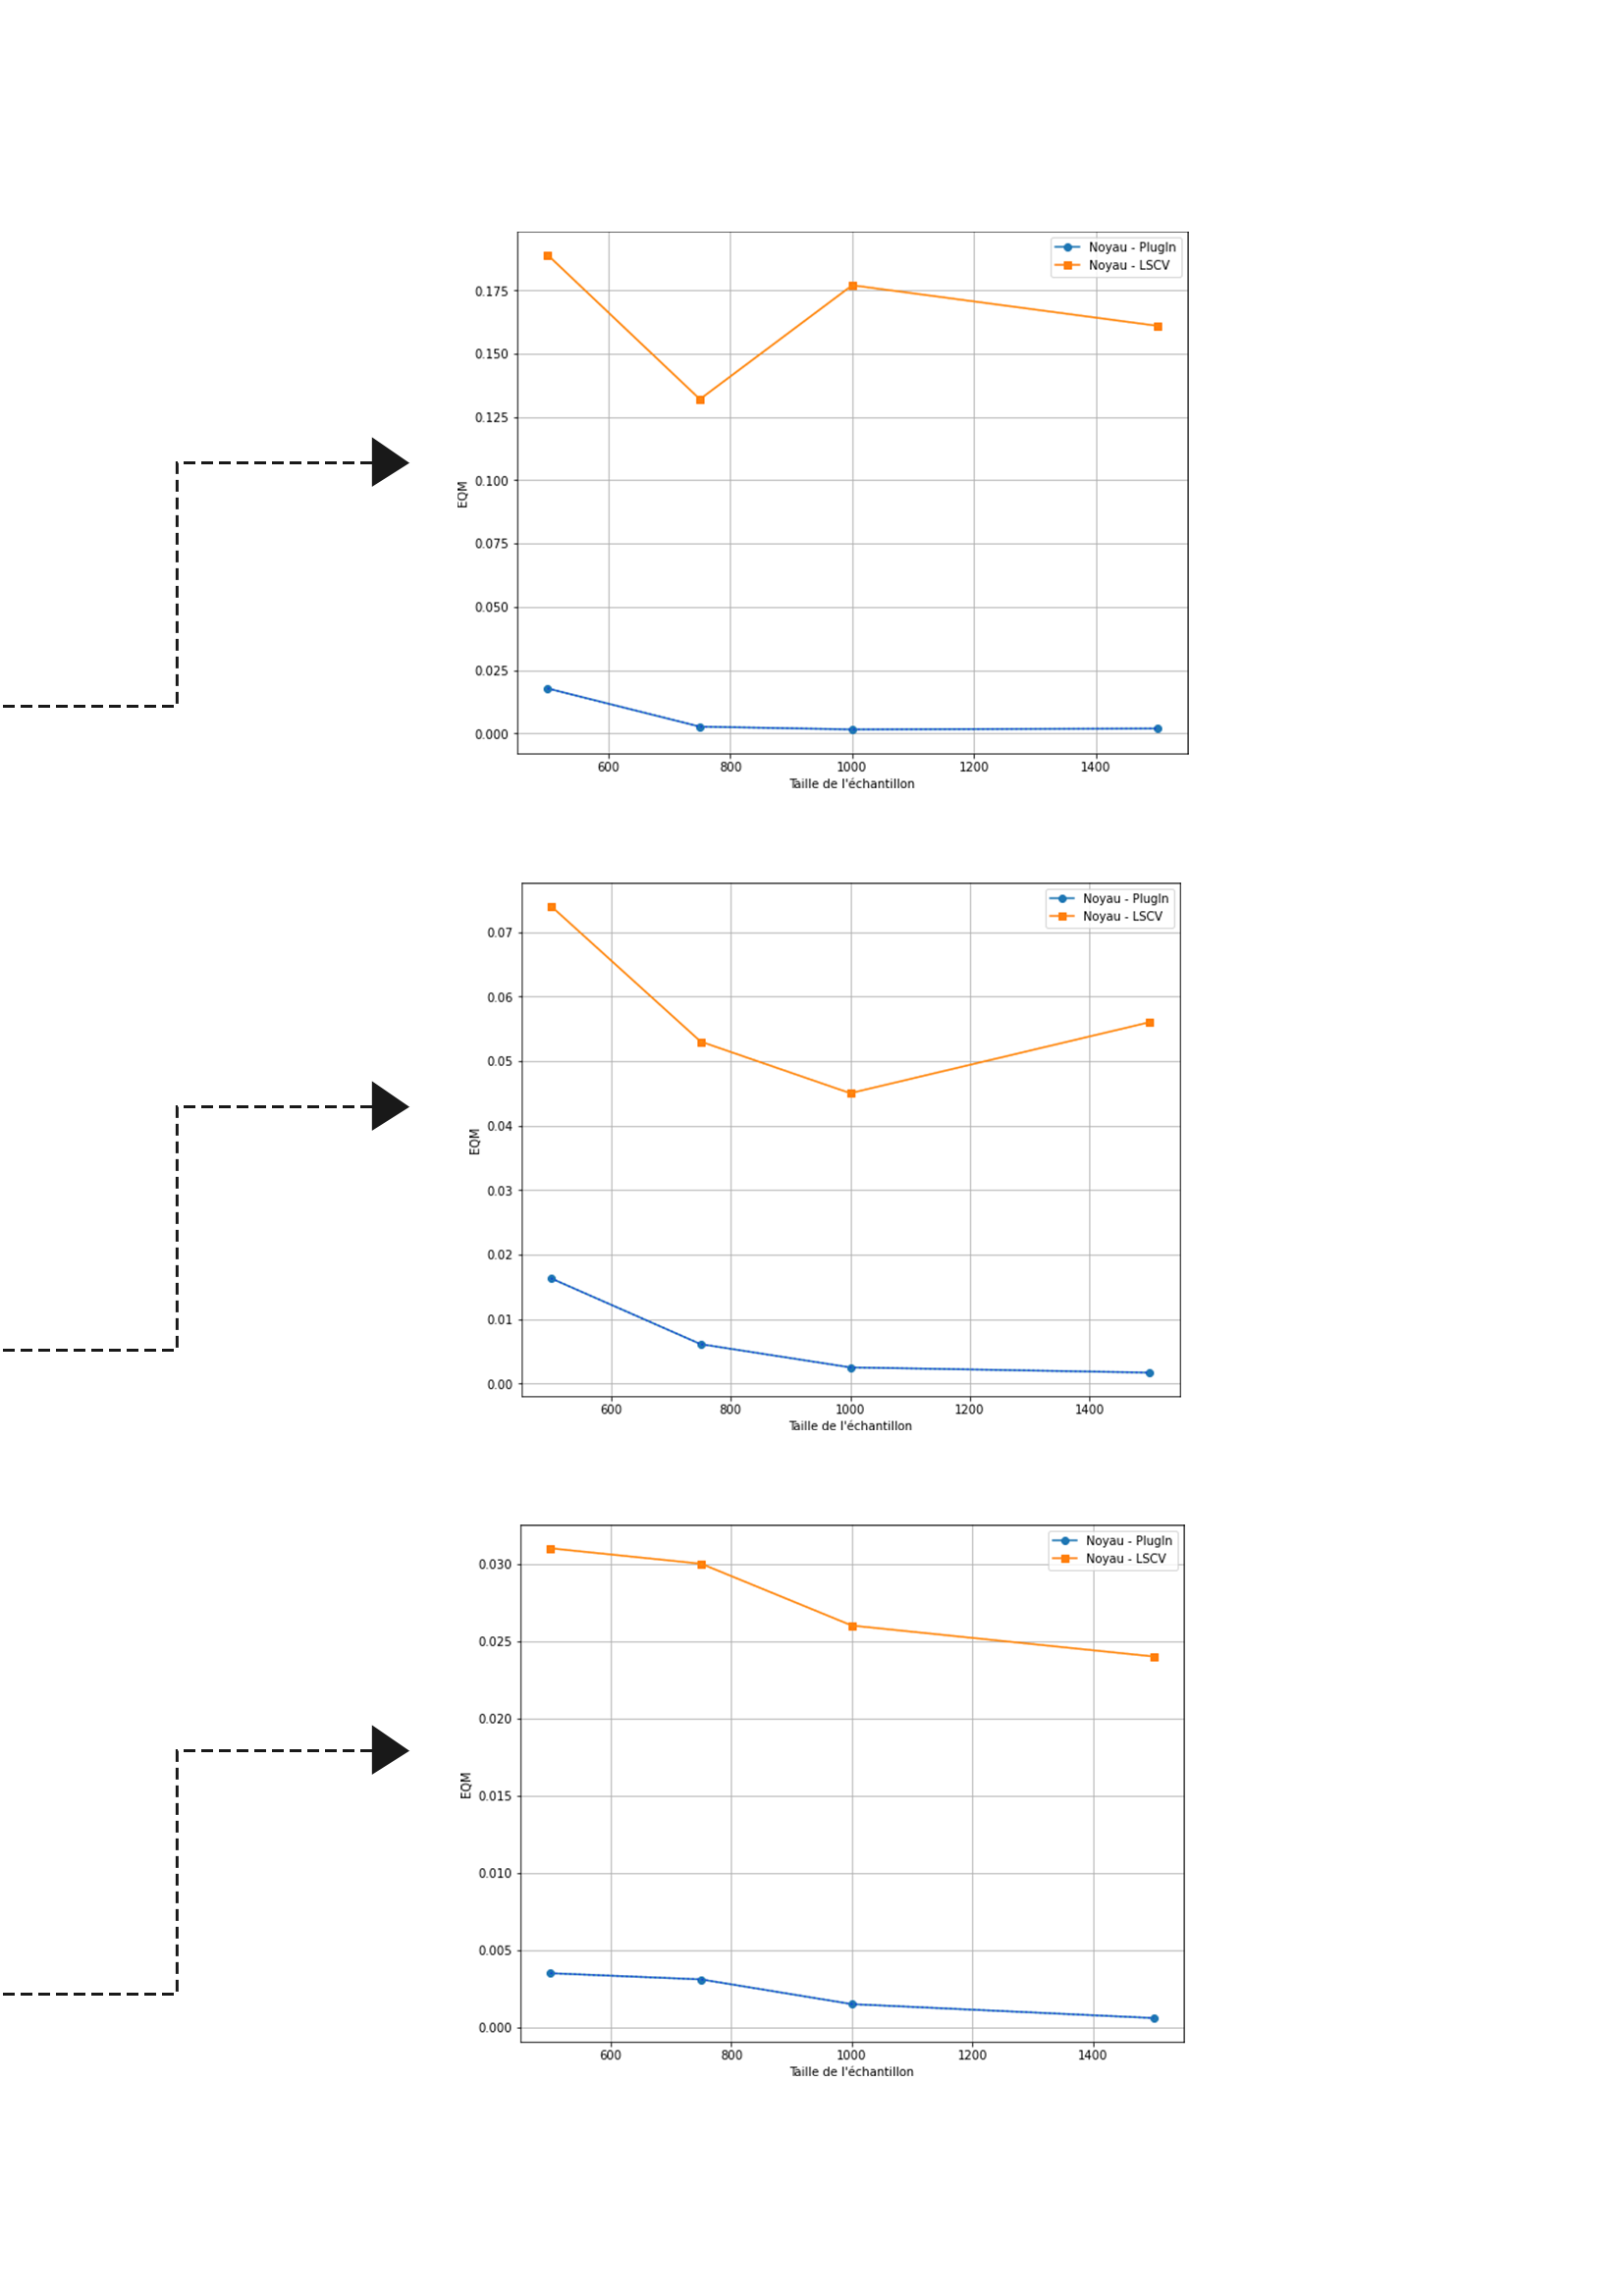
\includegraphics[width=\textwidth]{P 02.png}
  \caption{EQM : G1-G2-G3}
  \label{fig:G1-G2-G3}
\end{figure}
\begin{figure}[!h]
  \centering
  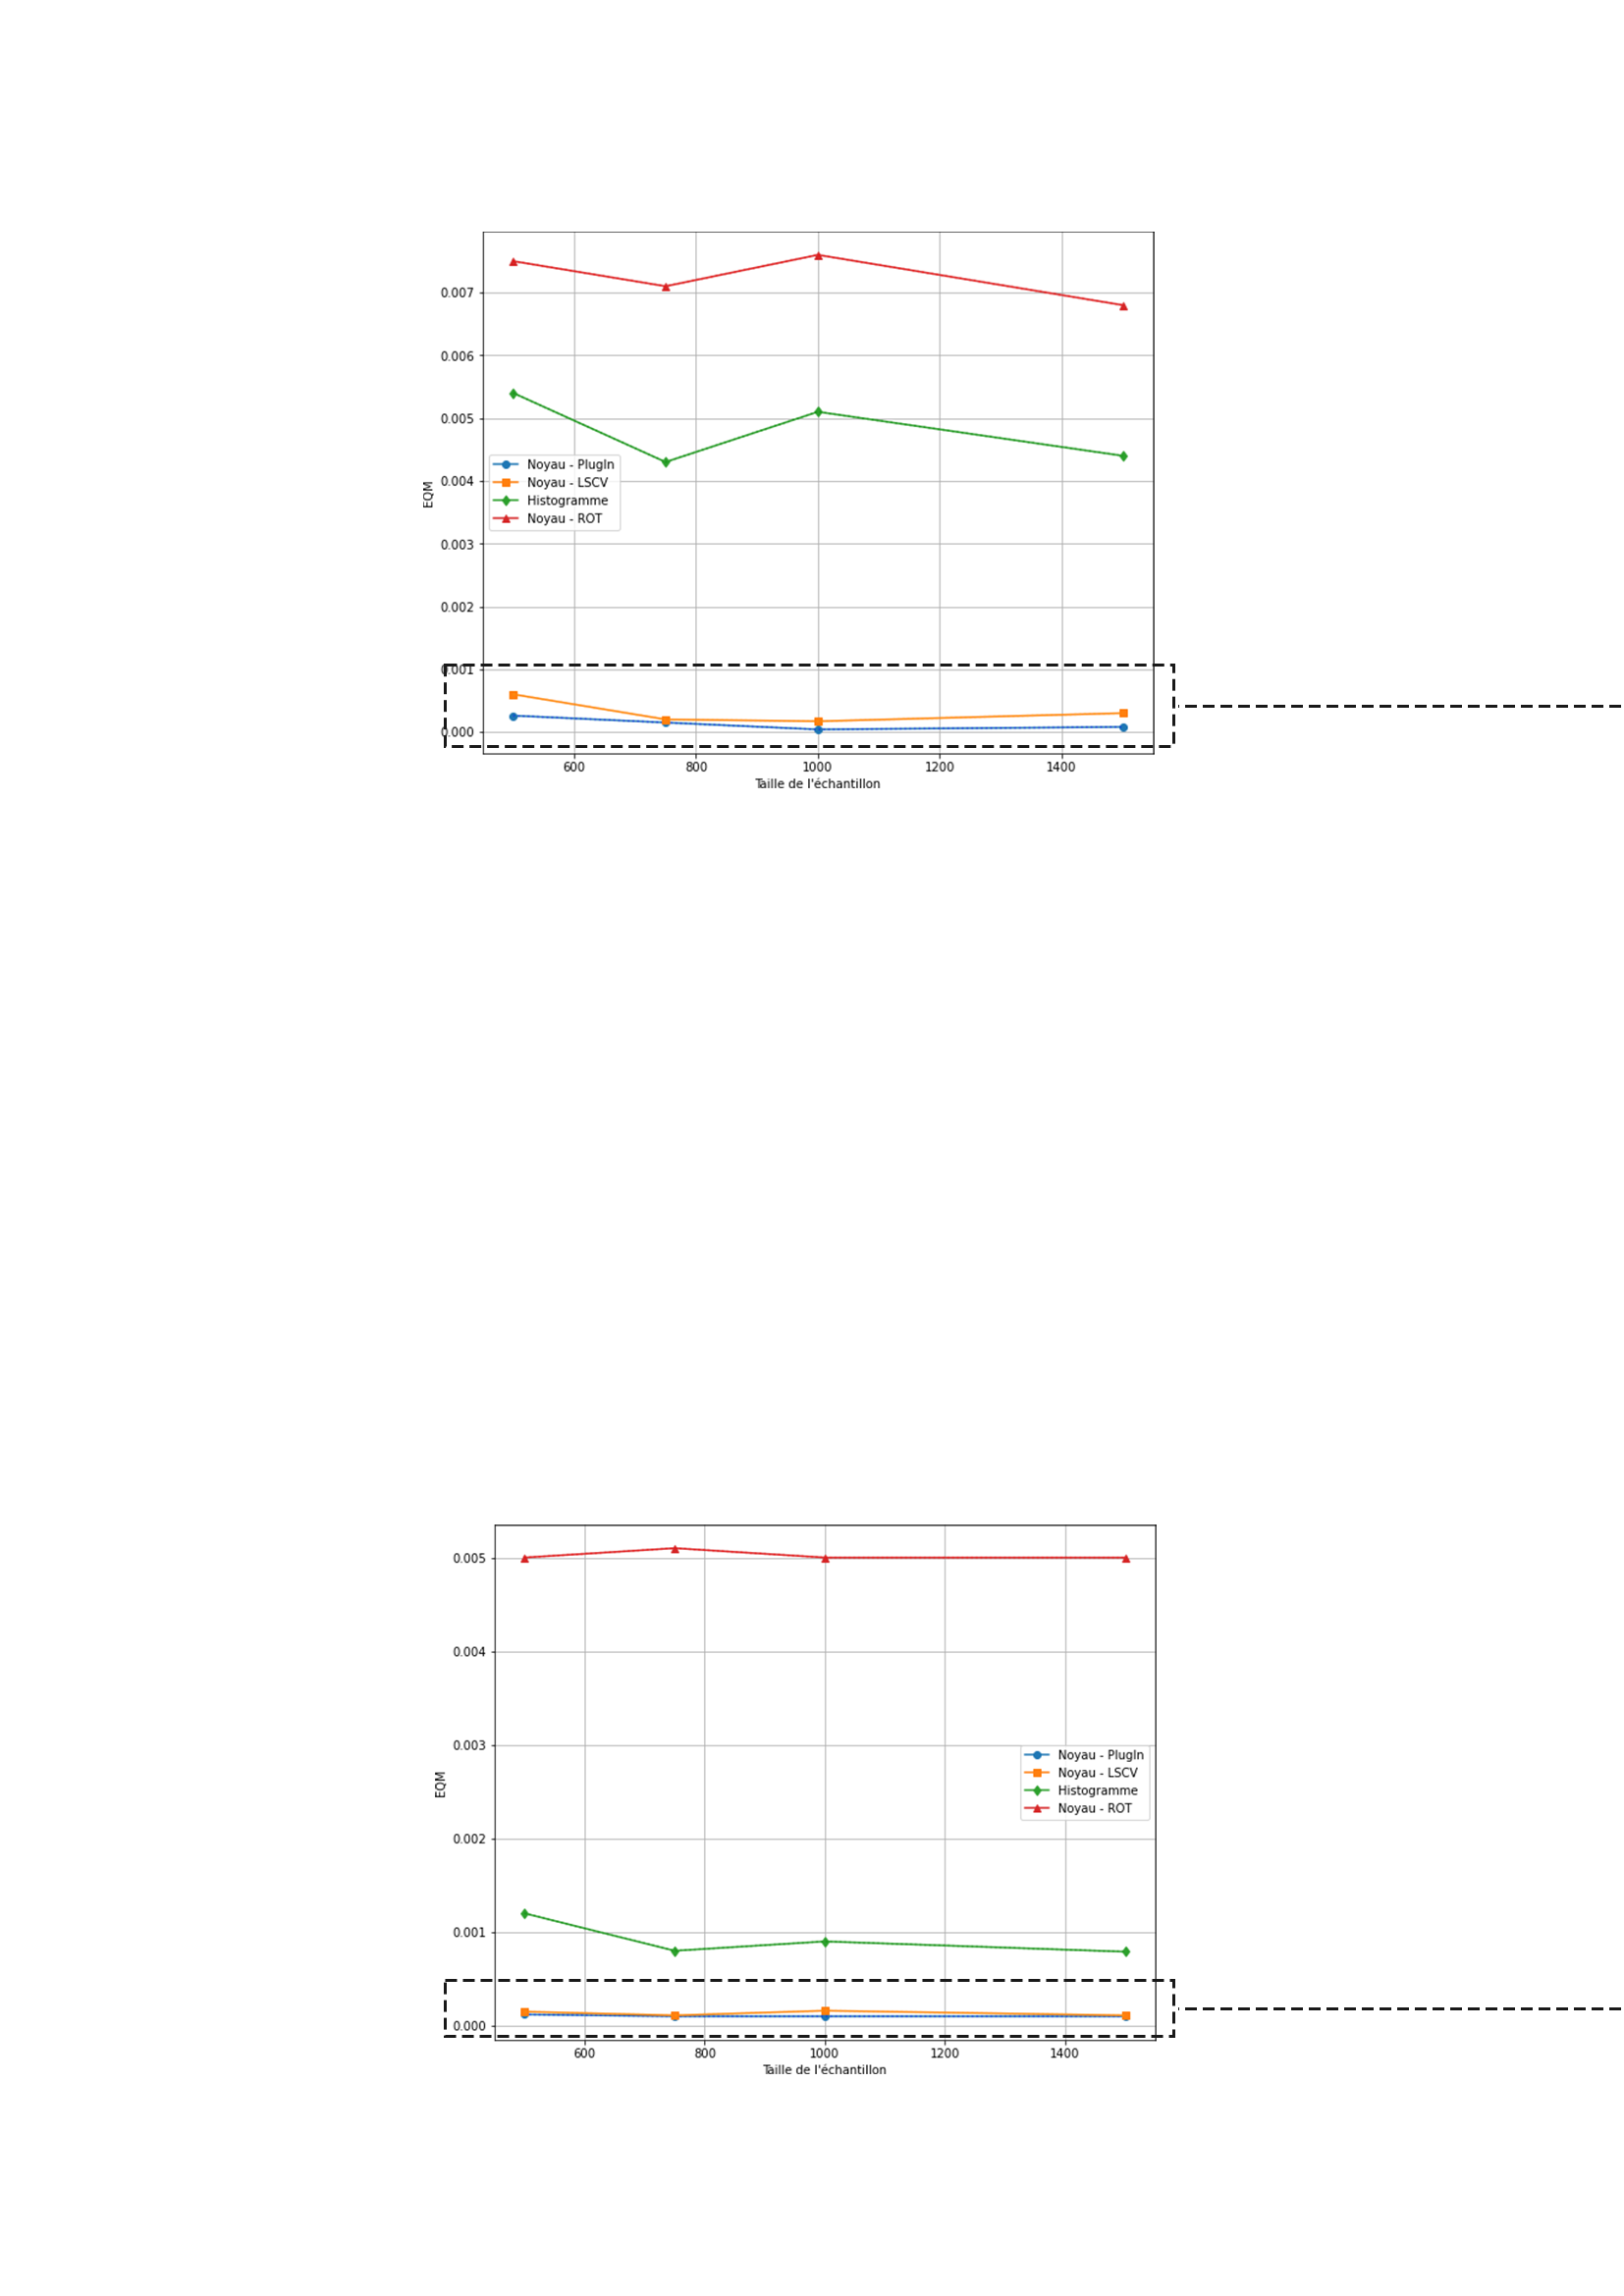
\includegraphics[width=\textwidth]{P 03.png}
  \caption{EQM  G4-G5}
  \label{fig:G4-G5}
\end{figure}
\begin{figure}[!h]
  \centering
  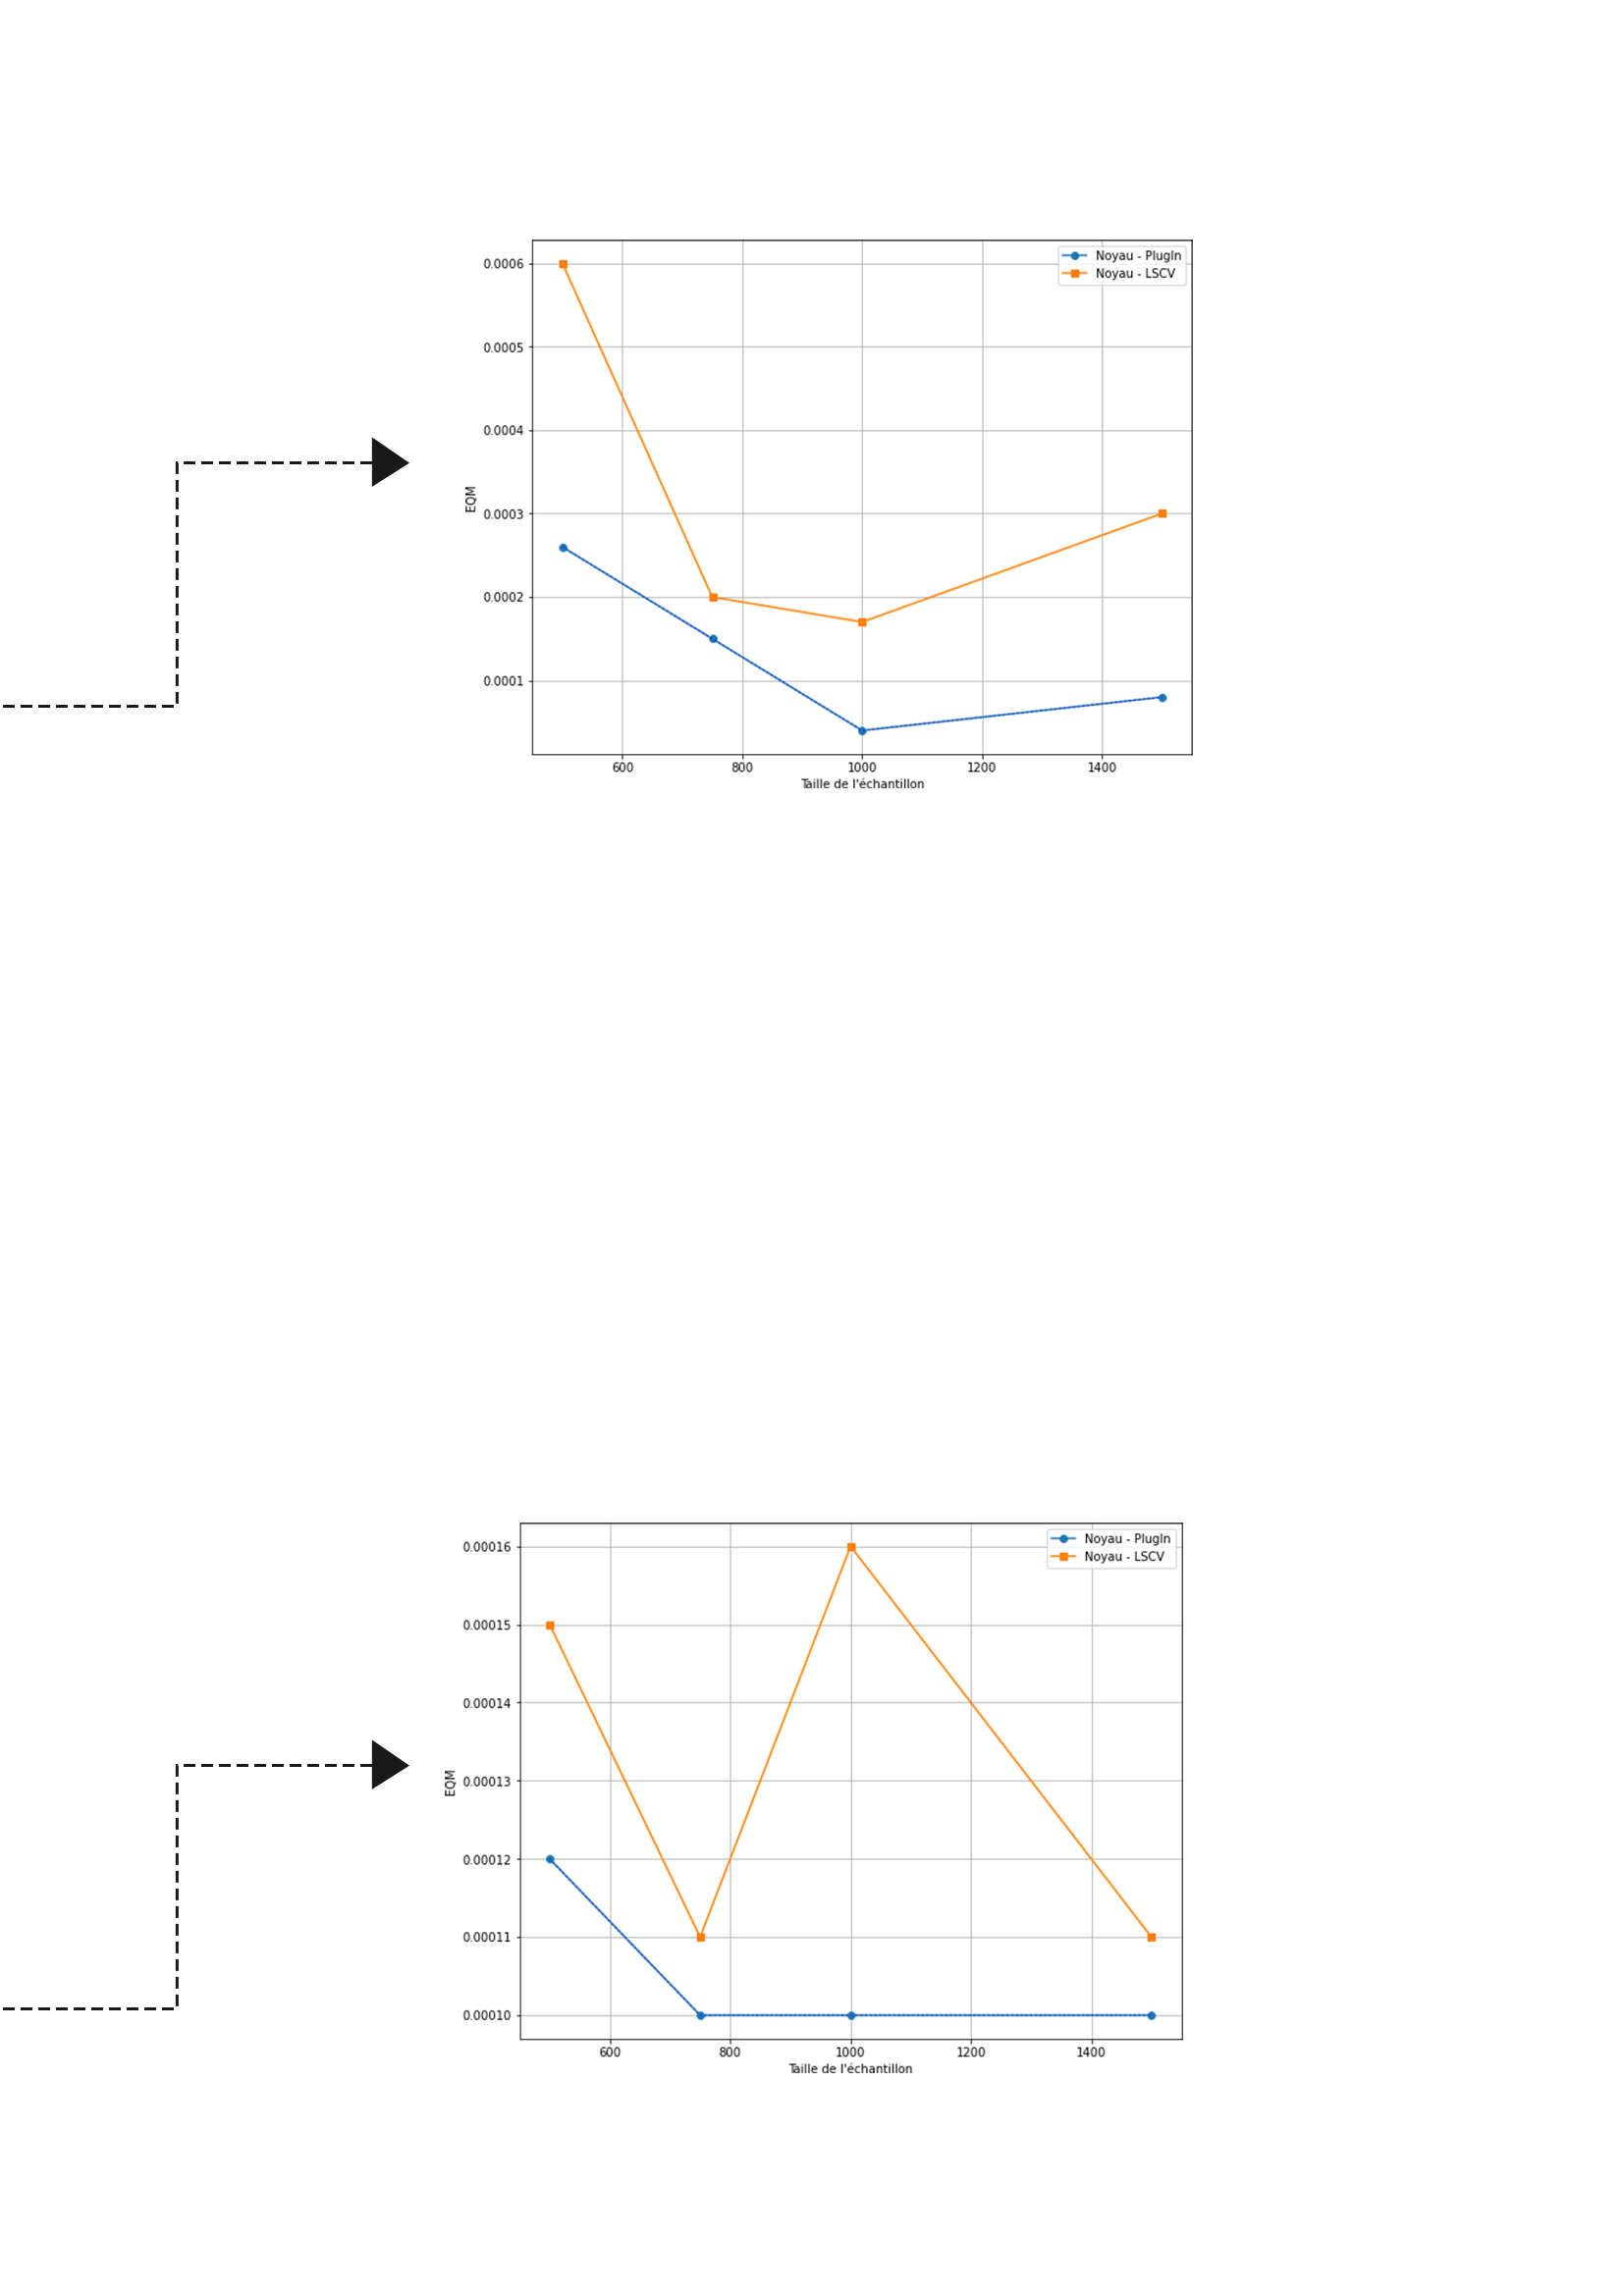
\includegraphics[width=\textwidth]{P 04.png}
  \caption{EQM : G4-G5}
  \label{fig:G1-G2-G3}
\end{figure}
\clearpage
\section{Interprétations}
L'analyse des résultats montre que la méthode de Plug-in noyau présente des performances généralement supérieures aux autres méthodes en termes d'erreur quadratique moyenne (EQM) pour les cinq distributions étudiées. Cela peut s'expliquer par le fait que la méthode de Plug-in noyau utilise une estimation non paramétrique de la ddp en ajustant un noyau à chaque point de données, ce qui peut permettre de mieux capturer la structure sous-jacente de la distribution réelle. En revanche, les autres méthodes telles que la méthode ROT, qui est implémentée par défaut en Python, peuvent avoir des limitations dans la capacité à estimer avec précision les densités de probabilité pour des distributions complexes ou multimodales.
 
Il est intéressant de noter que pour les distributions de type loi normale, l'EQM diminue au fur et à mesure que l'on passe d'une distribution uni-modale à une distribution bi ou tri modale pour les méthodes d'optimisation de paramètre de lissage. Cela peut s'expliquer par le fait que les distributions bimodales ou tri-modales présentent des caractéristiques plus complexes avec des pics multiples, ce qui peut rendre l'estimation de la ddp plus difficile pour certaines méthodes. Cependant, l'algorithme de Plug-in semble mieux s'ajuster au pas optimal des distributions complexes, permettant d'atteindre des EQM plus faibles.

Il est également intéressant de noter que la taille de l'échantillon semble jouer un rôle important dans la précision des estimations. En effet, l'EQM diminue généralement avec l'augmentation de la taille de l'échantillon pour les simulations étudiées. En effet, des échantillons plus grands permettent d'obtenir plus d'information sur la distribution réelle et permettent ainsi d'obtenir des estimations plus précises de la ddp.

En ce qui concerne la comparaison entre la méthode de Plug-in noyau et la méthode LSCV,  ces deux méthodes présentent des performances similaires, pour les distributions uni-modales cependant un EQM toujours légèrement supérieur pour l'algorithme plug-in 

Enfin, la méthode de l'histogramme présente de bonnes performances en termes d'EQM pour toutes les distributions étudiées, tout en étant simple à implémenter. Bien que l'histogramme puisse présenter des limitations en termes de résolution et de lissage de la distribution, notamment pour les distributions complexes, il peut être suffisamment précis pour des distributions plus simples et présenter un bon compromis entre simplicité d'implémentation et précision des estimations.

En conclusion, les résultats obtenus montrent que la méthode de Plug-in noyau est généralement meilleure en termes d'EQM par rapport aux autres méthodes étudiées, notamment pour les distributions tri-modales. Cependant, la taille de l'échantillon et la complexité de la distribution peuvent également jouer un rôle important dans la précision des estimations. La méthode LSCV présente des performances similaires à la méthode de Plug-in noyau, mais peut sous-estimer la complexité de la distribution réelle. La méthode de l'histogramme présente également de bonnes performances en termes d'EQM pour certaines distributions notamment la loi uniforme, tout en étant simple à implémenter. Enfin, il est important de noter que le choix de la méthode d'estimation de densité de probabilité dépendra des caractéristiques spécifiques de la distribution étudiée, de la taille de l'échantillon disponible, ainsi que des objectifs de l'analyse statistique ou de la modélisation.

Donc on peut dire que la méthode noyau Plug-in est la plus précise et la plus robuste.

\section{Conclusion}
Dans ce chapitre, nous avons examiné plusieurs méthodes non paramétriques d'estimation de densité de probabilité et avons comparé leurs performances à l'aide de simulations pour cinq distributions différentes. Les résultats montrent que la méthode noyau Plug-in est la plus précise et la plus robuste pour estimer les densités de probabilité pour les distributions étudiées. Les méthodes LSCV, histogramme et ROT ont également donné des résultats satisfaisants, mais avec des degrés de précision différents en fonction de la distribution.

Ces résultats montrent que les méthodes non paramétriques sont des outils utiles pour estimer les densités de probabilité, en particulier lorsque la distribution est inconnue ou ne peut pas être décrite par une distribution paramétrique. Cependant, il est important de choisir la méthode appropriée en fonction de la précision souhaitée et de la robustesse aux différentes formes de distribution.

En conclusion, la méthode noyau Plug-in est la méthode la plus précise et la plus robuste, mais les autres méthodes peuvent également être utilisées avec des résultats satisfaisants, en fonction de la distribution et de l'objectif de l'analyse.
\newpage
\thispagestyle{empty}
\null\newpage


\clearpage

\chapter{Application sur la base d'images MNIST}
\section{Introduction}
Dans ce chapitre, nous introduisons une approche novatrice pour évaluer les performances d'un classifieur en prenant en compte la distribution de la précision. Lors de l'évaluation d'un modèle, il est essentiel de considérer la variabilité des performances d'une exécution à l'autre, notamment en fonction de l'échantillon d'apprentissage et des hyperparamètres choisis, tels que le nombre d'époques.

Pour remédier à cette problématique et obtenir une évaluation plus fiable, nous proposons d'utiliser les densités de probabilité des taux de précision comme métrique d'évaluation. Cette approche permet de prendre en compte la distribution de la précision dans l'analyse des performances du modèle.

Dans cette étude, nous appliquons cette approche à l'ensemble de données MNIST en utilisant la méthode du noyau avec l'algorithme Plug-in pour estimer les densités de probabilité des précisions de prédiction. Nous nous concentrons plus particulièrement sur l'impact du nombre d'époques sur la précision d'un classifieur CNN profond.

Pour évaluer cette influence, nous exécutons plusieurs fois le CNN en faisant varier les échantillons d'apprentissage. Cela nous permet de générer un échantillon de 100 précisions, considérées comme des réalisations indépendantes d'une variable aléatoire continue.

En utilisant la méthode du noyau avec optimisation du paramètre de lissage via l'algorithme Plug-in, nous estimons les distributions des précisions pour chaque valeur d'époque. Cette approche nous permet de comparer objectivement les performances du CNN en fonction des différentes valeurs d'époques.

En résumé, notre approche innovante consiste à évaluer les performances d'un classifieur en tenant compte de la distribution de la précision. Nous utilisons la méthode du noyau avec l'algorithme Plug-in pour estimer les densités de probabilité des précisions d'un modèle d'apprentissage automatique sur MNIST, en mettant l'accent sur l'influence du nombre d'époques sur la précision d'un CNN profond. Cette approche nous permet d'obtenir une évaluation plus objective et précise des performances du modèle.





\section{Base d'images MNIST}

Nous avons choisi la base de données MNIST pour tester notre méthode d'estimation de ddp non paramétrique. Cette base de données est bien connue dans la communauté de l'apprentissage automatique et se compose de 70 000 images de chiffres manuscrits de 0 à 9, chacune étant une image en niveaux de gris de 28 pixels sur 28 pixels.  Les images sont étiquetées avec les chiffres correspondants de 0 à 9. Cette variété d'images en fait un choix idéal pour tester la performance de notre méthode.

\begin{figure}[!h]
  \centering
  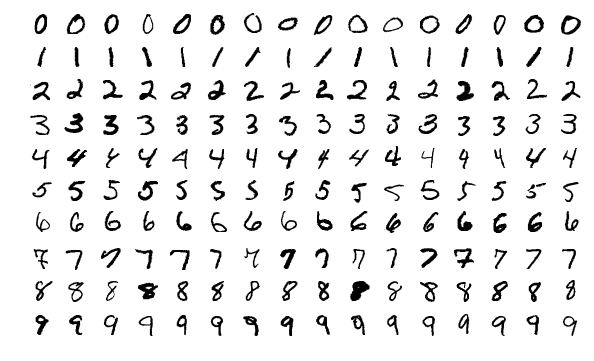
\includegraphics[width=\textwidth]{Figure 4.1.png}
  \caption{Extrait de la BD MNIST}
  \label{fig:Extrait de la BD MNIST}
\end{figure}
\clearpage 
\section{Modèle d’apprentissage}
Pour appliquer cette méthode noyau plug-in à un exemple pratique, nous avons choisi d'utiliser un modèle de réseau de neurones convolutionnel. Les CNN sont un type de modèle de ML particulièrement adapté pour les tâches de classification d'images. Les CNN ont prouvé leur efficacité dans la classification d'images en apprenant à extraire des caractéristiques pertinentes à partir des données d'entrée.

\subsection{Optimiseur: ADAM}
Dans le cas de la base de données MNIST, la nature des données est relativement simple en termes de complexité et de variabilité. Cela signifie que nous n'avons pas besoin d'un optimiseur complexe pour obtenir de bonnes performances. Cependant, ADAM (Adaptive Moment Estimation) est un choix raisonnable car il permet une convergence rapide et stable pour les modèles de réseau de neurones, ce qui est important pour obtenir une précision élevée tout en évitant le sur-apprentissage.\\ ADAM combine deux techniques d'optimisation, à savoir la méthode du gradient stochastique (SGD) et l'estimation des moments d'ordre supérieur des gradients. En utilisant ces deux techniques, ADAM peut adapter de manière adaptative le taux d'apprentissage pour chaque paramètre du modèle en fonction de son historique de gradient. En outre, ADAM maintient également une estimation des seconds moments du gradient, ce qui permet une normalisation de la mise à l'échelle des gradients et une amélioration de la convergence.

\subsection{Architecture du modèle}
Notre modèle CNN utilise 8 couches empilées les unes sur les autres :

\begin{lstlisting}
model = keras.Sequential(
        [
            keras.Input(shape=input_shape),
            layers.Conv2D(32, kernel_size=(3, 3), activation="relu"),
            layers.MaxPooling2D(pool_size=(2, 2)),
            layers.Conv2D(64, kernel_size=(3, 3), activation="relu"),
            layers.MaxPooling2D(pool_size=(2, 2)),
            layers.Flatten(),
            layers.Dropout(0.5),
            layers.Dense(num_classes, activation="softmax"),
        ]
                            )
\end{lstlisting}
\begin{figure}[!h]
  \centering
  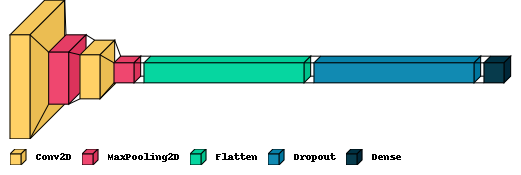
\includegraphics[width=\textwidth]{ModelView.png}
  \caption{ Model View à l'aide de Visualkeras}
  \label{fig:Model View à l'aide de Visualkeras}
\end{figure}

\begin{itemize}
    \item \textbf{La première couche}, $keras.Input(shape=inputshape)$, est une couche d'entrée qui spécifie la forme des données d'entrée. Ici, $input_shape$ correspond à la forme de chaque image d'entrée. Dans le cas de MNIST, chaque image est une matrice de 28x28 pixels en niveaux de gris, donc $inputshape=(28, 28, 1)$.
    \vspace{0.5cm}
    \item \textbf{La deuxième couche}, $layers.Conv2D(32, kernel_size=(3, 3), activation="relu")$, est une couche de convolution qui applique 32 filtres de convolution de taille 3x3 à l'image d'entrée. La fonction d'activation "relu" est utilisée pour introduire une non-linéarité dans les sorties de la couche de convolution.
        \vspace{0.5cm}
    \item \textbf{La troisième couche}, $layers.MaxPooling2D(poolsize=(2, 2))$, est une couche de pooling qui réduit la taille de la sortie de la couche de convolution en conservant uniquement la valeur maximale de chaque fenêtre de 2x2 pixels. Cette opération permet de réduire le nombre de paramètres du modèle et d'introduire une certaine invariance à la translation dans les sorties de la couche de convolution.
        \vspace{0.5cm}
    \item \textbf{La quatrième couche}, $layers.Conv2D(64, kernelsize=(3, 3), activation="relu")$, est une deuxième couche de convolution qui applique 64 filtres de convolution de taille 3x3 à la sortie de la couche de Pooling précédente.
            \vspace{0.5cm}

     \item \textbf{La cinquième  couche}, $layers.MaxPooling2D(poolsize=(2, 2))$, est une deuxième couche de Pooling qui réduit de nouveau la taille de la sortie de la deuxième couche de convolution.
         \vspace{0.5cm}
    \item \textbf{La sixième   couche}, $layers.Flatten()$, transforme la sortie de la deuxième couche de Pooling en un vecteur à une dimension, qui peut être alimenté dans des couches entièrement connectées.
        \vspace{0.5cm}
    \item \textbf{La septième couche},$layers.Dropout(0.5)$, est une couche de régularisation qui supprime aléatoirement certains neurones avec une probabilité de 0,5. Cette opération aide à prévenir le sur-apprentissage du modèle.
        \vspace{0.5cm}
     \item \textbf{La dernière   couche}, $layers.Dense(numclasses, activation="softmax")$, est une couche entièrement connectée qui calcule une probabilité pour chaque classe de sortie. Ici, $numclasses$ est le nombre de classes de sortie, qui est égal à 10 pour MNIST. La fonction d'activation "$softmax$" est utilisée pour s'assurer que la somme des probabilités pour chaque classe est égale à 1. 
\end{itemize}
\subsection{Métrique d'évaluation de la performance}
Nous avons choisi d'opter pour le taux de précision comme évaluateur de performance pour notre modèle, en raison de certaines caractéristiques importantes. Lorsque nous examinons la surface d'une densité de taux de performance, nous constatons qu'elle tend vers l'infini, ce qui indique une excellente capacité de prédiction. En revanche, la densité des taux d'erreurs tend vers zéro, ce qui suggère une faible propension à commettre des erreurs.

Cette observation nous oblige à utiliser un noyau de déformation pour garantir une bonne correspondance entre les prédictions du modèle et les valeurs réelles. Pour ce faire, nous utiliserons le taux de précision comme indicateur de performance du modèle. En utilisant un noyau conventionnel par la suite, nous pourrons mettre en œuvre les étapes nécessaires pour atteindre nos objectifs, comme nous l'expliquerons dans la section suivante.

La précision mesure le pourcentage d'images correctement classées. C’est est une métrique couramment utilisée pour évaluer les performances d'un modèle de ML. Elle mesure le nombre de prédictions correctes effectuées par le modèle sur l'ensemble des prédictions. La formule pour calculer la précision est : \\

\textbf{Précision = nombre de prédictions correctes / nombre total de prédictions}

\section{Méthodologie}
Pour évaluer la performance de notre modèle, nous avons mis en place une méthodologie rigoureuse en suivant les étapes suivantes :
\begin{enumerate}
    \item Nous avons effectué 100 itérations de l'apprentissage sur la base de données MNIST, pour chaque valeur d'époque fixe.
    \item À chaque itération, nous avons mélangé les données pour obtenir un ensemble de test différent de l'ensemble d'entraînement de la dernière itération, ce qui permet d'éviter obtention les même valeurs de précisions.
    \item À chaque itération, nous avons également stocké la valeur de la précision obtenue lors de la phase de validation dans une liste dédiée.
    \item Toutes les 100 itérations, nous avons augmenté la valeur de l'époque pour tester notre modèle avec les valeurs suivantes : [5, 10, 15, 20, 25, 30, 40].
    \item Cette procédure nous a permis d'obtenir sept listes de 100 valeurs de précision de validation pour chaque époque testée.
    \item Comme chaque liste de valeurs est considérée comme une variable aléatoire, étant donné que le mélange des données se fait de manière aléatoire et que les images dans l'ensemble d'entraînement sont également aléatoires, la précision obtenue est elle aussi aléatoire.\\ Nous avons donc appliqué la méthode de noyau Plug-in sur chacune des listes de précision (variables aléatoires) pour estimer la densité de probabilité de la précision pour les époques 5 à 40.
    \\
\end{enumerate}
\section{Résultats}
La figure ci-dessous présente les résultats de notre travail, montrant l'estimation de la densité de probabilité de la précision pour les époques 5 à 40 à l'aide de la méthode de noyau Plug-in
\clearpage
\begin{figure}[!h]
  \centering
  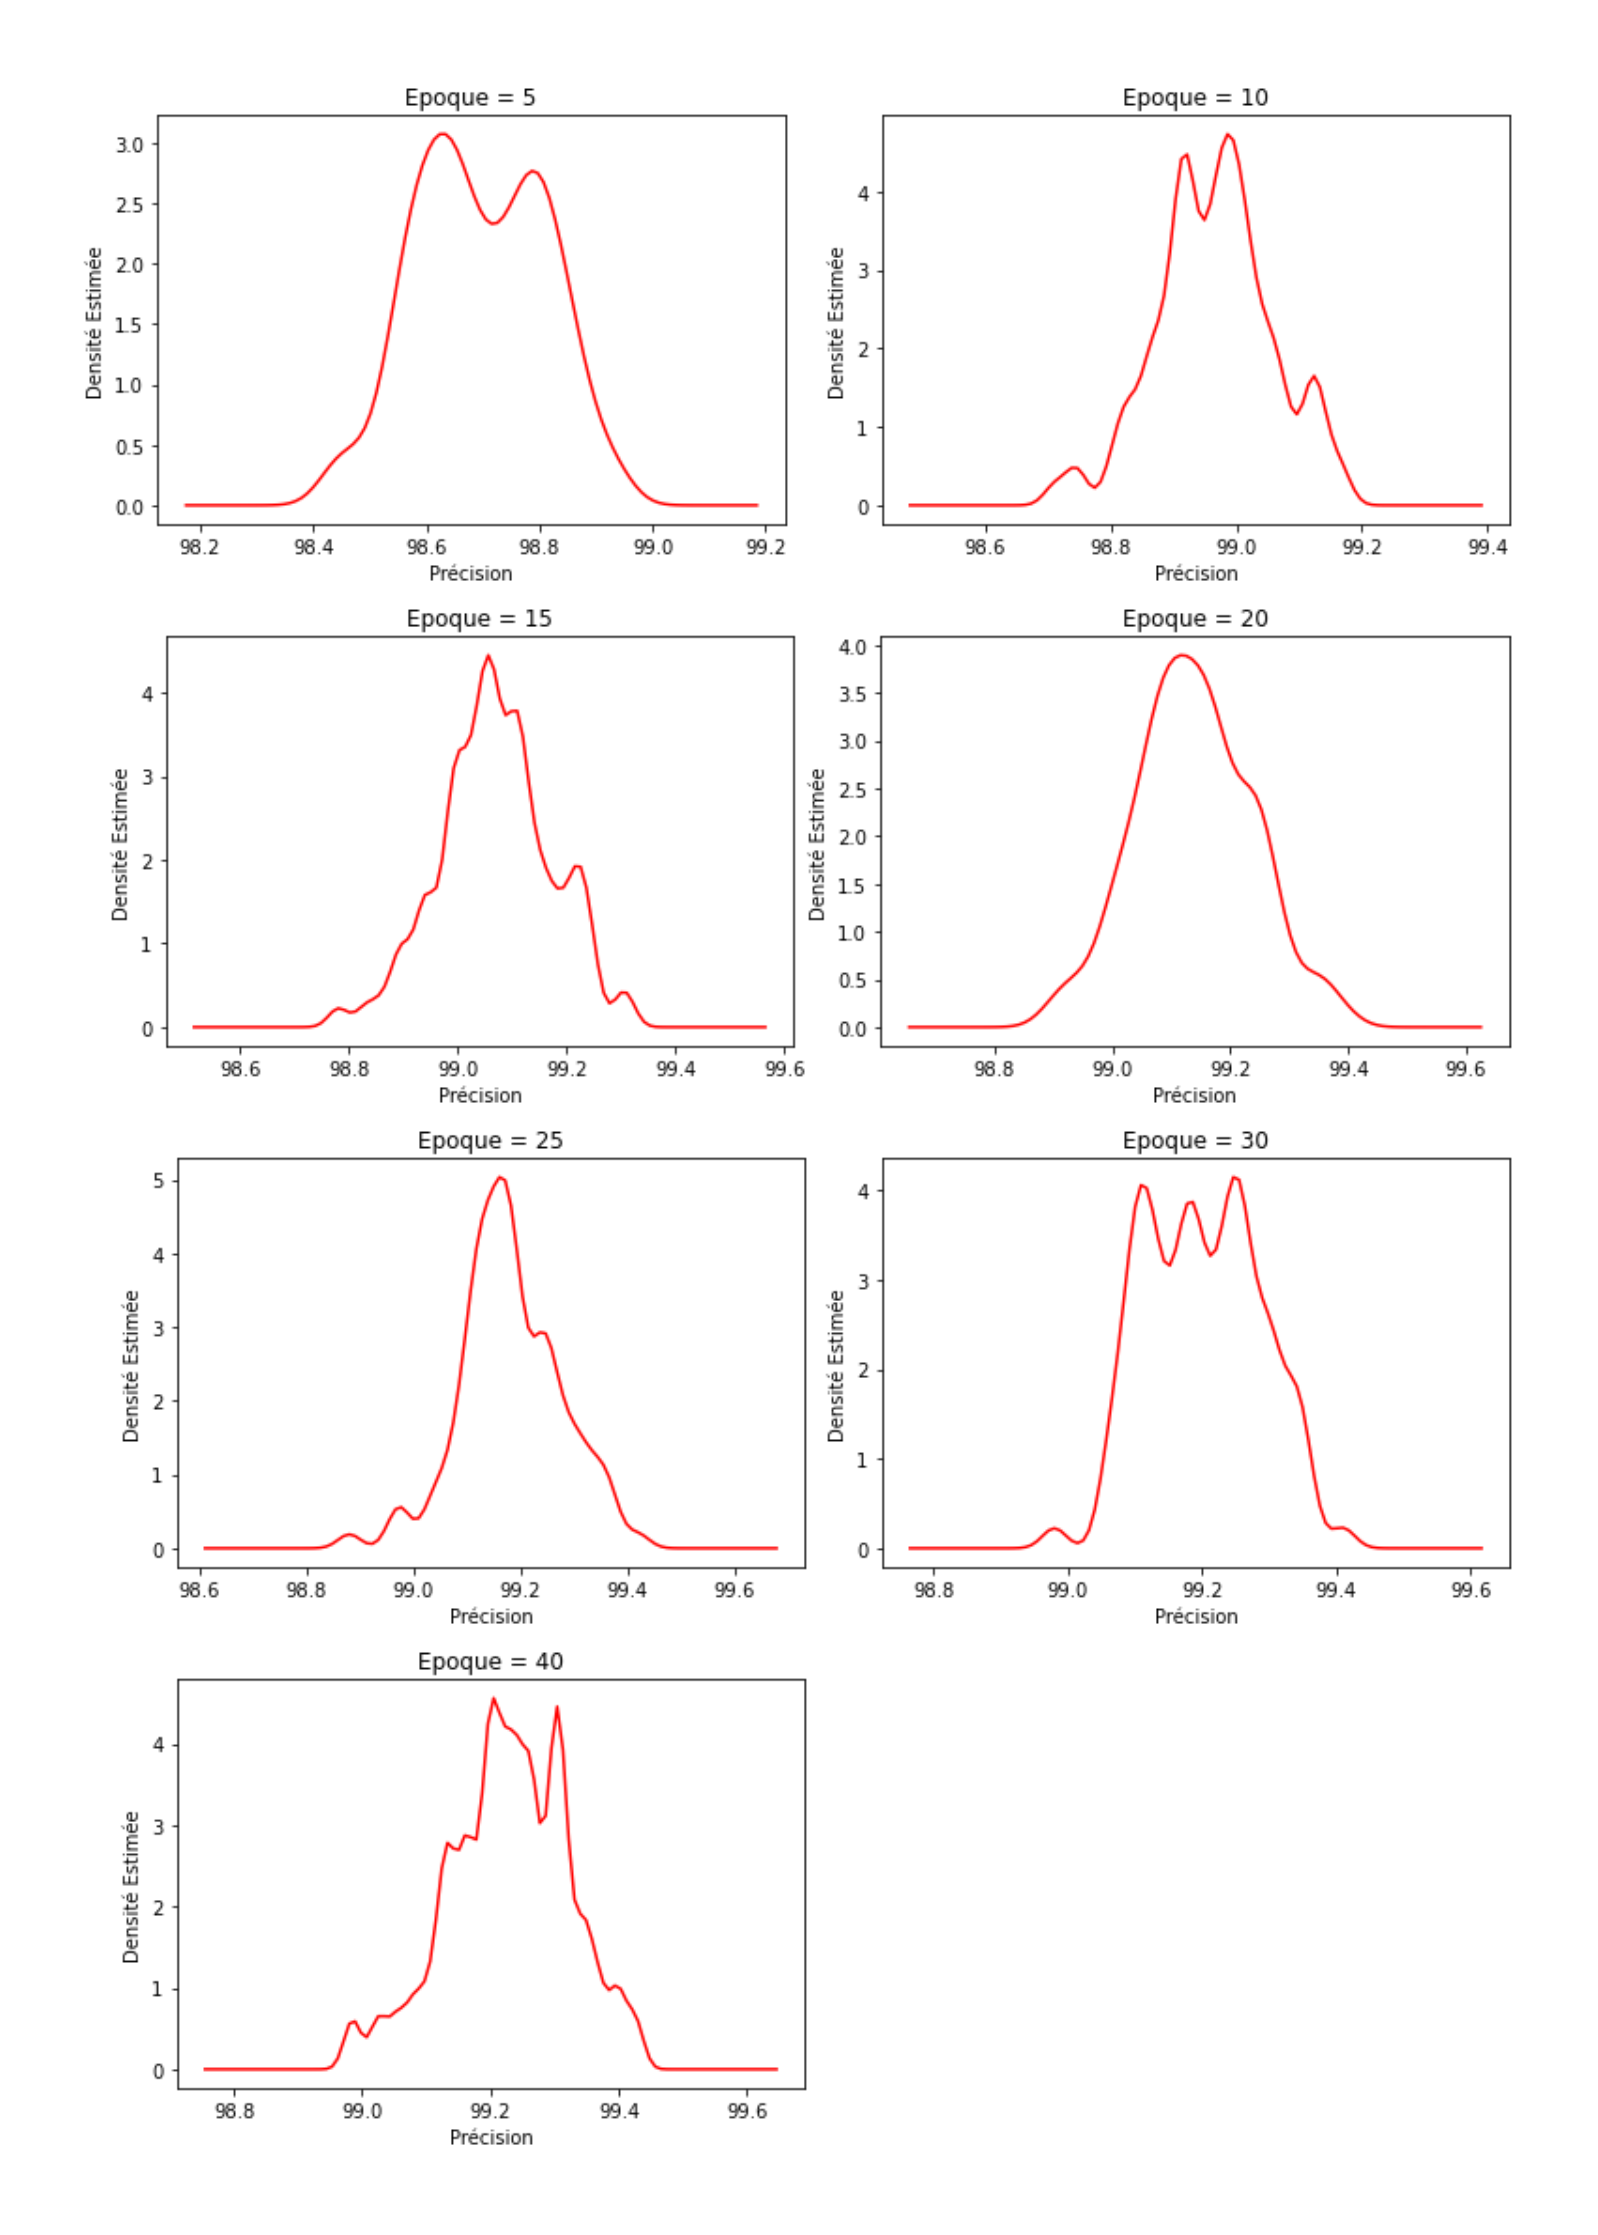
\includegraphics[width=16cm,height=21cm]{Figure 4.2.png}
  \caption{Densités estimées avec noyau Plug In}
  \label{fig:Densités estimées avec noyau Plug In}
\end{figure}
\clearpage
L'objectif de la figure suivante est de déterminer la moyenne des précisions obtenues au début et de comparer les densités par rapport à cette moyenne.

Pour ce faire, nous calculons la surface sous la courbe de densité à partir de la moyenne et en allant vers l'infini (puisque nous avons utilisé les taux de précision). Cette surface nous permet de déterminer la probabilité qu'une densité soit supérieure à la moyenne des précisions. Cette probabilité sera calculée en utilisant l'approximation des trapèzes.
\clearpage

\begin{figure}[!h]
  \centering
  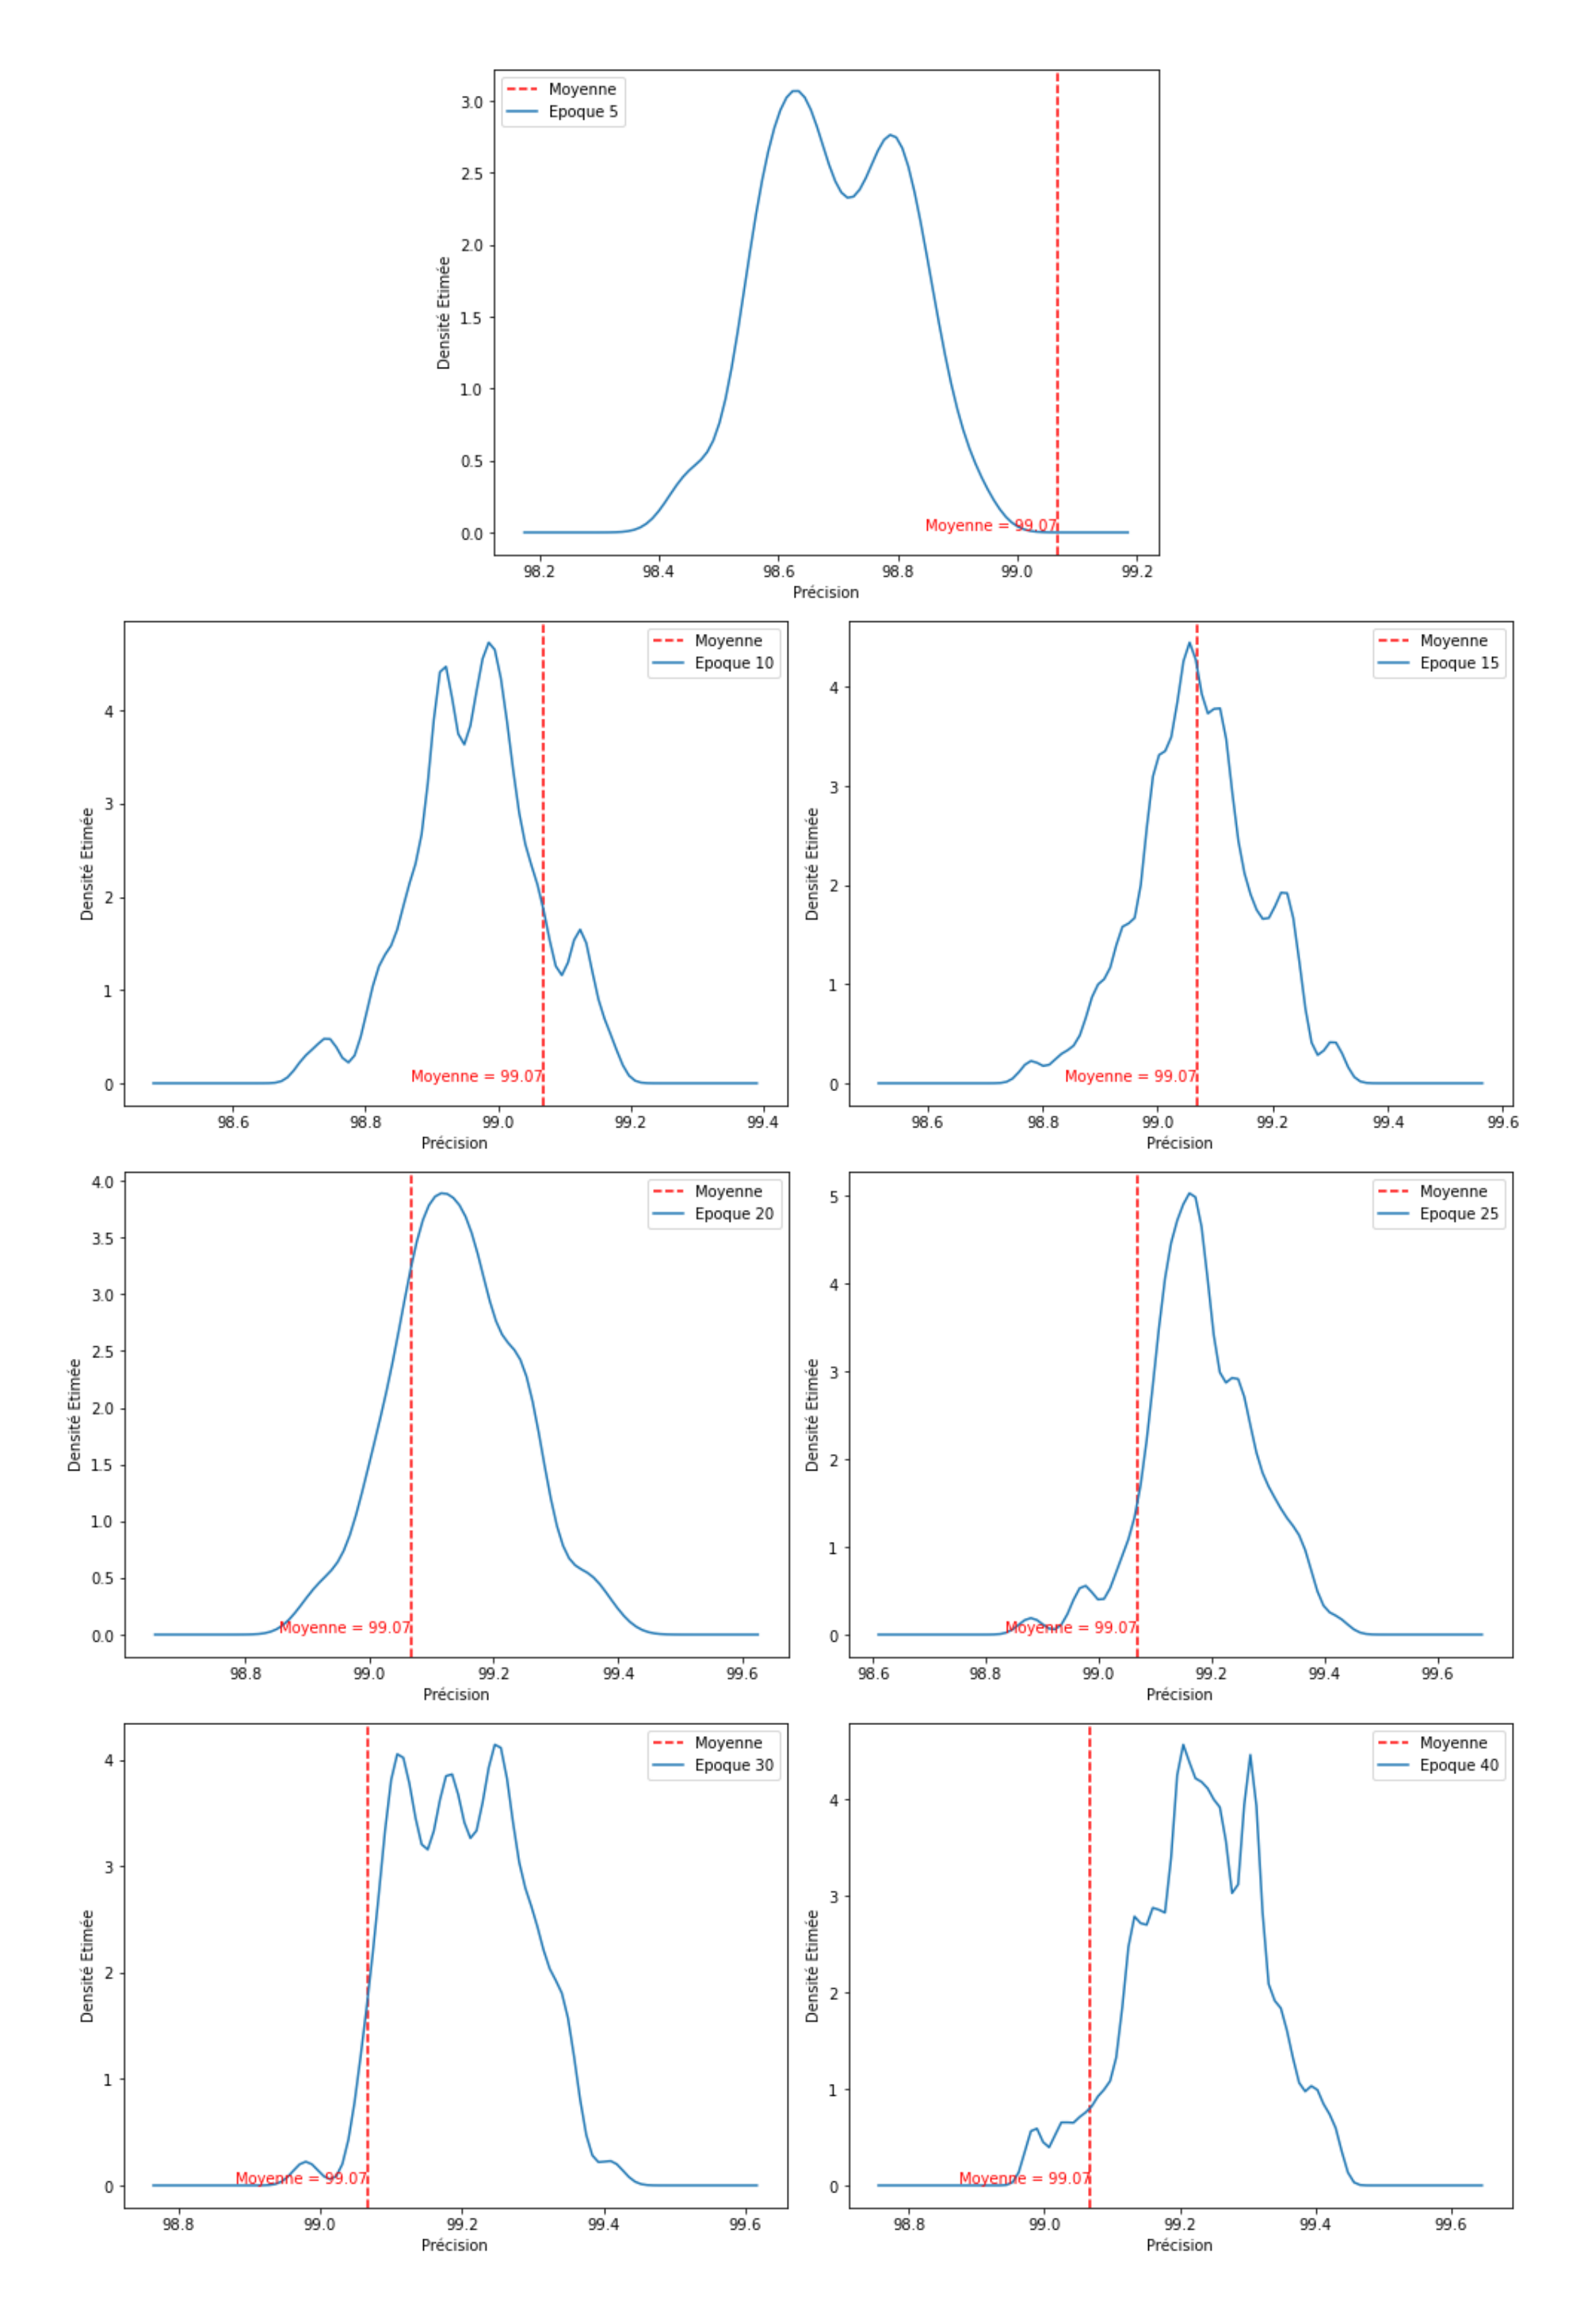
\includegraphics[width=16cm,height=21cm]{Figure 4.3.png}
  \caption{Comparaison avec la moyenne de précisions}
  \label{fig:Comparaison avec la moyenne de précisions}
\end{figure}
\clearpage
Voici une implémentation en Python 3 de la logique précédemment expliquée pour calculer la probabilité que la précision 
dépasse la moyenne des précisions : \\
$P[accuracy > m]$
\newline
Avec m : la moyenne des précisions.

\begin{lstlisting}
def calculer_surface_sous_courbe(x, y):
    # x : tableau des valeurs x de la courbe
    # y : tableau des valeurs y de la courbe

    if len(x) != len(y):
        raise ValueError("Les tableaux x et y doivent avoir la meme longueur.")

    # Calculer la surface sous la courbe par l'approximation des trapezes
    surface = np.trapz(y, x)

    return surface

num_epochs = [5, 10, 15, 20, 25, 30, 40]

for epoch in num_epochs:
    support = globals()[f"support{epoch}"] 
    epoch_sup_a_moyenne = [num for num in support if num > mean_of_means]
    deniste_sup_a_moyenne = globals()[f"Y_estimated_{epoch}"][-len(epoch_sup_a_moyenne):]

   
    print(calculer_surface_sous_courbe(epoch_sup_a_moyenne, deniste_sup_a_moyenne))
         Y[-1] = Y[-1] / (c*n*hn)
        e = -100
        d = 100
        I = 0
        Jf = 0
        z = 0
        for k in range(1, P-2):
            z = (Y[k+1]-2*Y[k]+Y[k-1])
            I += z**2
        I = I + ((Y[P-2])**2 + (Y[P-2]-2*Y[P-3])**2) / (r**4)
        #Estimation de Jf 
        Jf = I / (r**3)
        
    return Y


\end{lstlisting}
 \vspace{1cm}
 Les surfaces obtenues sont:
       \vspace{0.25cm}

 \begin{itemize}
     \item Pour le classifieur 1 ( Époque : 5 ) = $7.735e-07$ 
      \vspace{0.25cm}

    \item Pour le classifieur 2 ( Époque : 10 ) = $0.137$
      \vspace{0.25cm}

     \item Pour le classifieur 3 ( Époque : 15 ) = $0.454$ 
      \vspace{0.25cm}

     \item Pour le classifieur 4 ( Époque : 20 ) = $0.717$ 
      \vspace{0.25cm}

     \item Pour le classifieur 5 ( Époque : 25 ) = $0.887$ 
      \vspace{0.25cm}

     \item Pour le classifieur 6 ( Époque : 30 ) = $0.933$ 
      \vspace{0.25cm}

     \item Pour le classifieur 7 ( Époque : 40 ) = $0.928$ 

 \end{itemize}





\clearpage
\section{Discussion}
Dans notre expérience, nous avons étudié l'impact de différentes valeurs d'époque sur les estimations de densité des précisions pour un modèle d'apprentissage automatique entraîné sur l'ensemble de données MNIST.

En analysant les résultats, nous avons constaté que l'époque joue un rôle crucial dans la répartition de l'estimation de densité des précisions. À mesure que la valeur d'époque augmente, la densité se répartit davantage et couvre l'ensemble de l'image. Cela suggère que la précision du modèle d'apprentissage automatique s'améliore avec l'augmentation des valeurs d'époque, car le modèle est capable de capturer plus de caractéristiques dans l'ensemble de données.

Dans l'ensemble, nos estimations de densité des précisions suggèrent que l'époque=30 est la plus susceptible de produire la précision la plus élevée pour le modèle d'apprentissage automatique entraîné sur l'ensemble de données MNIST. Cette conclusion est étayée par l'utilisation de la métrique de probabilité, qui nous a permis de calculer la surface sous la courbe de densité en partant de la moyenne des précisions jusqu'à l'infini. Nous avons constaté que la densité du classifieur ayant une époque de 30 a donné la surface la plus élevée après la moyenne des précisions, ce qui suggère une précision relativement élevée et constante pour le modèle à cette époque.

En revanche, les estimations de densité pour les valeurs d'époque inférieures à 30 présentent une distribution relativement plate et diffuse, indiquant que la précision du modèle est plus variable et moins constante pour ces valeurs d'époque. De même, les estimations de densité pour les valeurs d'époque supérieures à 30 présentent des pics relativement étroits et plus bas, suggérant que la précision du modèle pourrait commencer à diminuer pour ces valeurs d'époque plus élevées.

En conclusion, nos résultats indiquent que l'époque=30 est un candidat prometteur pour atteindre une précision élevée pour le modèle CNN entraîné sur l'ensemble de données MNIST. Cependant, des analyses supplémentaires sont nécessaires pour confirmer cette conclusion et évaluer si des valeurs d'époque encore plus élevées pourraient éventuellement conduire à une diminution de la précision du modèle.
\newpage
\section{Conclusion}
En conclusion, notre étude a visé à déterminer l'époque optimale pour atteindre une précision élevée dans le modèle CNN entraîné sur l'ensemble de données MNIST. En utilisant des estimations de densité basées sur la métrique de probabilité, nous avons analysé les distributions des précisions pour différentes valeurs d'époque.

Cependant, des analyses supplémentaires sont nécessaires pour confirmer cette conclusion et évaluer si des valeurs d'époque encore plus élevées pourraient conduire à une diminution de la précision du modèle. Il est recommandé de poursuivre les recherches en examinant d'autres métriques et en effectuant des tests sur des ensembles de données supplémentaires pour une validation plus approfondie.

Dans l'ensemble, cette étude fournit des informations précieuses sur la sélection de l'époque optimale pour maximiser la précision dans le modèle d'apprentissage automatique. Ces résultats peuvent être utilisés pour améliorer les performances des modèles CNN dans diverses tâches de classification, y compris la reconnaissance de caractères et d'objets.
\newpage
\thispagestyle{empty}
\null\newpage







\clearpage

\chapter{Simulateur}
\section{Introduction}
La recherche en data science nécessite souvent l'estimation des densités de probabilités des données utilisés. Dans ce chapitre, nous présentons une application développée dans le but de permettre aux chercheurs d'estimer facilement les densités de probabilités à l'aide d'une interface graphique conviviale.

Notre application se compose de deux sections principales. Dans la première section, les utilisateurs peuvent importer leurs données, telles que des taux de précision, des taux d'erreur, etc., qui vont être considérées comme des variables aléatoires. L'application est ensuite en mesure d'estimer la densité de ces variables en les affichant graphiquement. Pour cette estimation, nous utilisons la méthode du noyau avec l'optimisateur de paramètre de lissage plug-in.

La deuxième section de l'application permet aux utilisateurs de mener des simulations de mélange de trois lois : normale, exponentielle ou uniforme, avec leurs paramètres respectifs. Ensuite, ils peuvent visualiser les densités estimées pour ces distributions en utilisant la méthode de l’histogramme et la méthode du noyau avec ROT, LSCV ou PLUG-IN pour la sélection du paramètre de lissage. De plus, l'application calcule également la densité réelle et EQM relatives aux différentes approches d'estimation. Cela permet de comparer éventuellement des données avec des modèles usuels.

L'application a été développée en utilisant le framework Angular pour la partie frontale et Flask pour la partie backend. Flask a été choisi car sa simplicité d'implémentation en fait un choix approprié. Angular, en tant qu'application SPA (Single Page Application) facilite la communication entre les composants et le chargement du contenu. De plus, il offre la possibilité d'intégrer des graphiques attrayants en utilisant les canvas pré-définis d'Angular. Ainsi, nous n'avons pas besoin d'appeler des graphiques depuis la bibliothèque Matplotlib. Nous pouvons simplement récupérer les listes des densités estimées à partir du backend Flask après le traitement et le calcul.

Ce chapitre présente donc en détail le développement et les fonctionnalités de cette application, ainsi que les résultats obtenus en utilisant différentes méthodes d'estimation pour diverses distributions.

\section{Technologies Utilisées}
Le développement de notre application s'appuie sur deux technologies clés : Angular pour la partie frontend et Python avec Flask pour la partie backend. Le choix de ces technologies a été motivé par leurs avantages spécifiques, qui ont contribué à la réalisation de notre objectif de créer une interface utilisateur conviviale et efficace pour l'estimation des densités de probabilités.
\subsection{Angular}
Angular est  connu pour être un framework de développement d'applications web monopage (SPA - Single-Page Application). Cela signifie que les applications Angular se chargent une seule fois dans le navigateur et mettent à jour dynamiquement le contenu de la page sans nécessiter de rechargement complet.
\subsubsection{Architecture}
Angular suit un modèle architectural appelé MVVM (Model-View-ViewModel), qui est une variante du MVC (Modèle-Vue-Contrôleur). Le MVVM est une conception architecturale qui sépare la logique métier (modèle), la présentation (vue) et la logique de liaison (ViewModel). Dans le MVVM d'Angular, le modèle représente l'état et la logique métier de l'application. La vue est responsable de l'affichage de l'interface utilisateur et de la réception des entrées de l'utilisateur. Le ViewModel agit comme une couche intermédiaire entre le modèle et la vue, gérant la logique de liaison de données, les événements et les interactions avec la vue.

Bien que le MVVM soit une variation du MVC, il diffère légèrement dans la façon dont les responsabilités sont réparties entre les différents éléments. Le ViewModel est plus étroitement lié à la vue, ce qui facilite la gestion de la liaison de données bidirectionnelle et des événements spécifiques à la vue.
\subsubsection{Pourquoi Angular?}
Angular a été choisi pour la partie frontend en raison de sa nature SPA. Cette architecture permet une expérience utilisateur fluide en chargeant une seule page HTML initiale et en mettant à jour dynamiquement le contenu sans recharger complètement la page. Cela offre une navigation rapide et une communication facile entre les composants de l'application. De plus, Angular offre une riche bibliothèque de composants et de directives pré-définis, ce qui facilite la création d'une interface utilisateur attrayante et interactive surtout qu'on va intégrer des graphiques.

\subsection{Flask}
Flask est un framework web minimaliste et puissant pour le développement d'applications web en Python. Il offre une approche simple et flexible pour la création de sites web et d'APIs, en mettant l'accent sur la modularité et la simplicité du code. Flask permet de créer rapidement des applications web légères et efficaces tout en offrant des fonctionnalités de base pour le routage, le rendu de templates et la gestion des formulaires.

\subsubsection{Architecture}
L'architecture de Flask suit le modèle de développement web appelé "modèle-vue-contrôleur" (MVC), bien que de manière plus légère et flexible par rapport à certains frameworks MVC complets. Flask encourage une structure de code modulaire et permet aux développeurs de choisir les outils et bibliothèques qu'ils préfèrent pour gérer les différentes parties de l'application.

\subsubsection{Pourquoi Flask?}
Flask a été choisi comme framework backend pour sa simplicité d'utilisation, sa légèreté et sa parfaite intégration avec Python. Cette combinaison nous a permis d'adopter une approche centrée sur les contrôleurs et les modèles en renvoyant des réponses JSON plutôt que de générer des vues HTML. Ainsi, nous avons pu concevoir une architecture efficace, tout en offrant une flexibilité aux utilisateurs pour choisir et visualiser les densités estimées pour différentes distributions. En résumé, le choix de Flask et Python nous a permis de développer rapidement une application avec des contrôleurs et des modèles, tout en fournissant des réponses JSON pour une expérience utilisateur fluide et une gestion simplifiée des données.




\section{Présentation de l'application}
\subsection{Description}
L'objectif de notre application est de mettre à la disposition des chercheurs un outil leur permettant d'estimer les densités de probabilités des variables aléatoires. Pour cela, nous utilisons la méthode du noyau avec une optimisation du paramètre de lissage en utilisant la méthode PLUG in. De plus, une partie de l'application vise à comparer les performances des estimateurs pour des lois usuelles.

La première fonctionnalité de l'application permet à l'utilisateur de faire des simulations en choisissant trois distributions (dont une est obligatoire et les deux autres optionnelles). Pour chaque distribution, l'utilisateur peut sélectionner l'une des trois lois disponibles : normale, exponentielle ou uniforme. De plus, il peut spécifier les paramètres de chaque distribution. Cette fonctionnalité donne à l'utilisateur la possibilité de jouer avec la complexité des distributions afin d'étudier plus précisément les performances des estimateurs. Les méthodes qui vont être utilisées dans les estimations sont la méthode du noyau ( ROT, LSCV et Plug-in) et la méthode de l'histogramme.

La deuxième partie de l'application permet à l'utilisateur de télécharger des fichiers texte contenant des valeurs, qui peuvent être des taux de précision d'un classifieur, par exemple, comme nous l'avons fait dans le chapitre précédent. Ensuite, la densité de probabilité de ces variables est calculée dans le backend de l'application et affichée dans un graphique pour l'utilisateur. L'utilisateur a également la possibilité de télécharger plusieurs fichiers et de travailler avec plusieurs variables, ce qui lui permet de visualiser les densités de ces variables sur le même graphique et de déterminer le meilleur classifieur, comme nous l'avons fait dans le chapitre précédent.

\subsection{Architecture}
    L'architecture de mon application est représentée dans la figure ci-dessous. Les composants utilisés en Angular et les modules en Flask sont représentés par des rectangles noirs. Les flèches indiquent les interactions entre les différents composants et modules. Les notes en jaune représentent les actions spécifiques réalisées dans chaque partie de l'application.
    
\begin{figure}[!h]
  \centering
  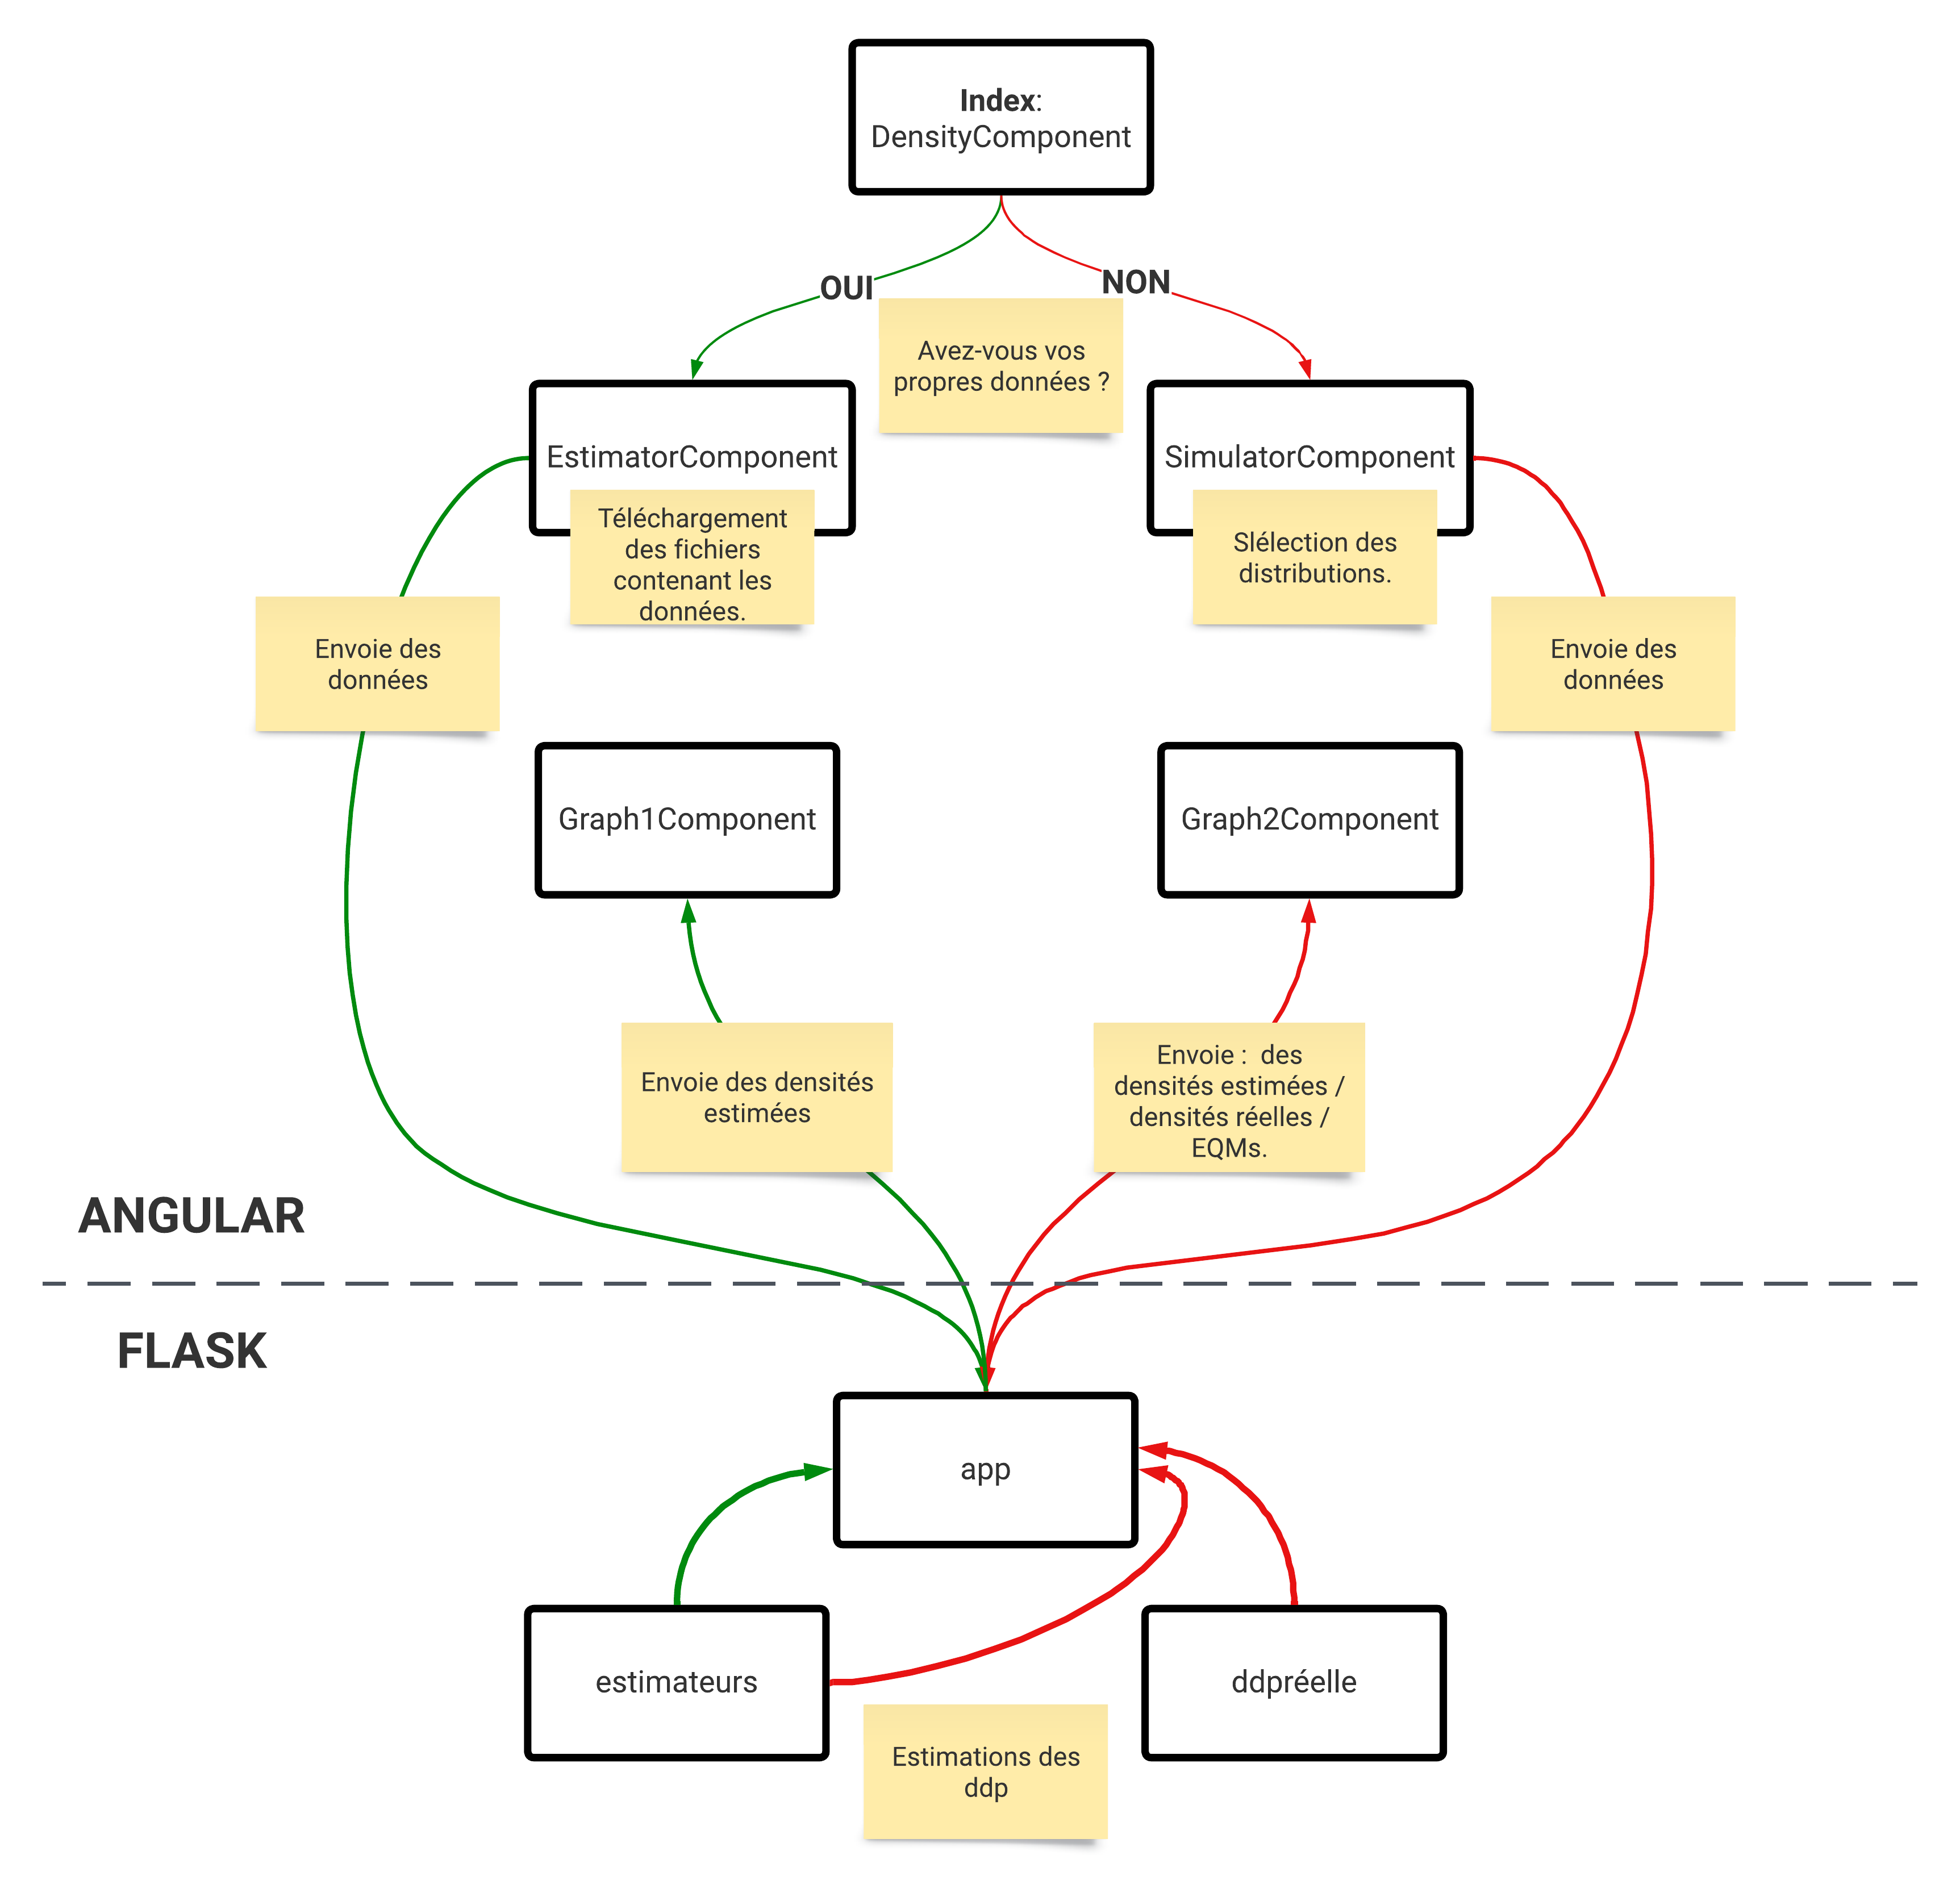
\includegraphics[width=18cm,height=21cm]{Figure 5.1.png}
  \caption{Architecture de l'application}
  \label{fig:Architecture de l'application}
\end{figure}
\clearpage

\section{Guide pratique}
En premier lieu, vous avez la possibilité de choisir entre deux options : importer vos propres données ou effectuer des simulations (voir Figure 5.2). Cette fonctionnalité vous offre une grande flexibilité en vous permettant de travailler avec vos propres données réelles ou de créer des scénarios simulés pour une analyse plus approfondie.

\begin{figure}[!h]
  \centering
  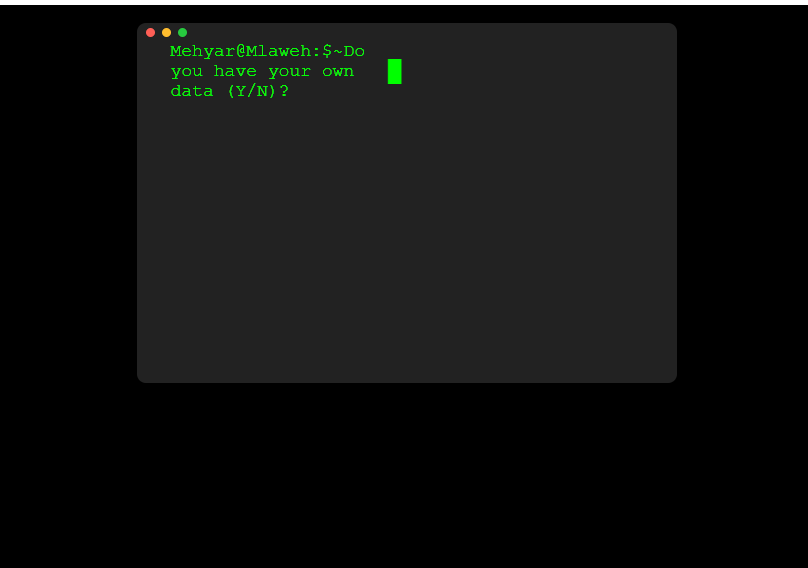
\includegraphics[width=15cm,height=10cm]{Figure 5.2.png}
  \caption{Page Index - Simulateur}
  \label{fig:Architecture de l'application}
\end{figure}

Dans la figure ci-dessous ( Figure 5.3), nous présentons la partie de l'application dédiée à la configuration des distributions à estimer. L'utilisateur a la possibilité de choisir jusqu'à trois distributions pour effectuer l'estimation, tandis que la deuxième et troisième distribution sont facultatives, offrant ainsi une flexibilité pour ajuster la complexité du mélange. Cette fonctionnalité permet à l'utilisateur de personnaliser les paramètres des distributions et d'explorer différents scénarios pour l'estimation. Et dans la figure 5.4, nous pouvons voir la densité réelle du mélange et les densités estimées par la méthode de l'histogramme et la méthode du noyau avec Plug-in , ROT et LSCV. 
\clearpage

\begin{figure}[!h]
  \centering
  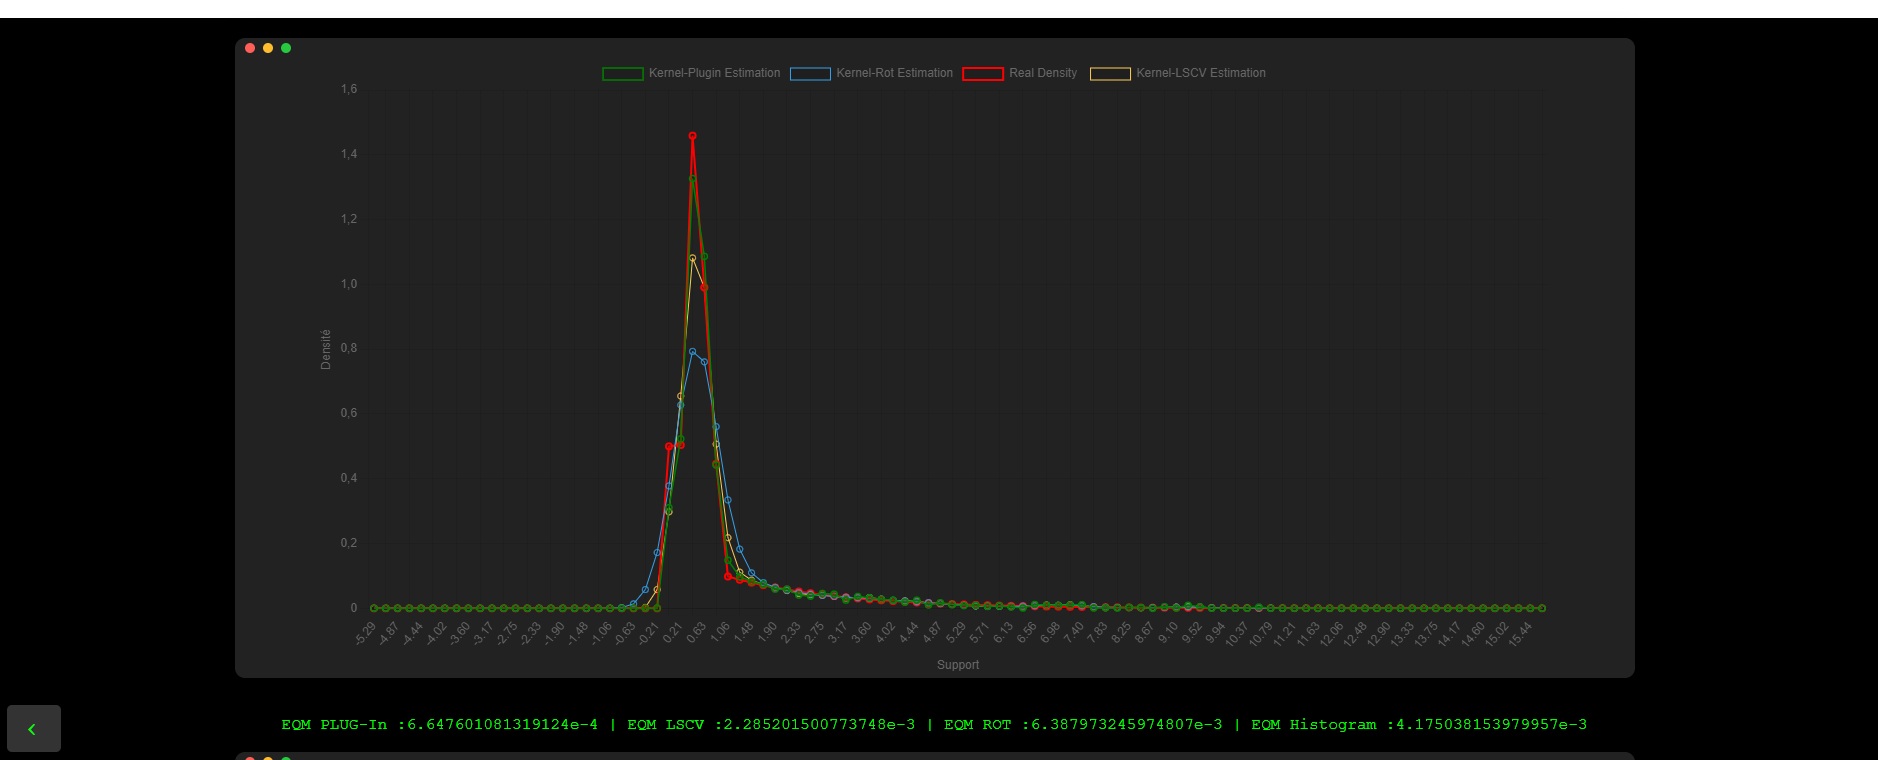
\includegraphics[width=15cm,height=9cm]{Figure 5.3.png}
  \caption{Choix des distributions - Simulateur}
  \label{fig:Architecture de l'application}
\end{figure}
\begin{figure}[!h]
  \centering
  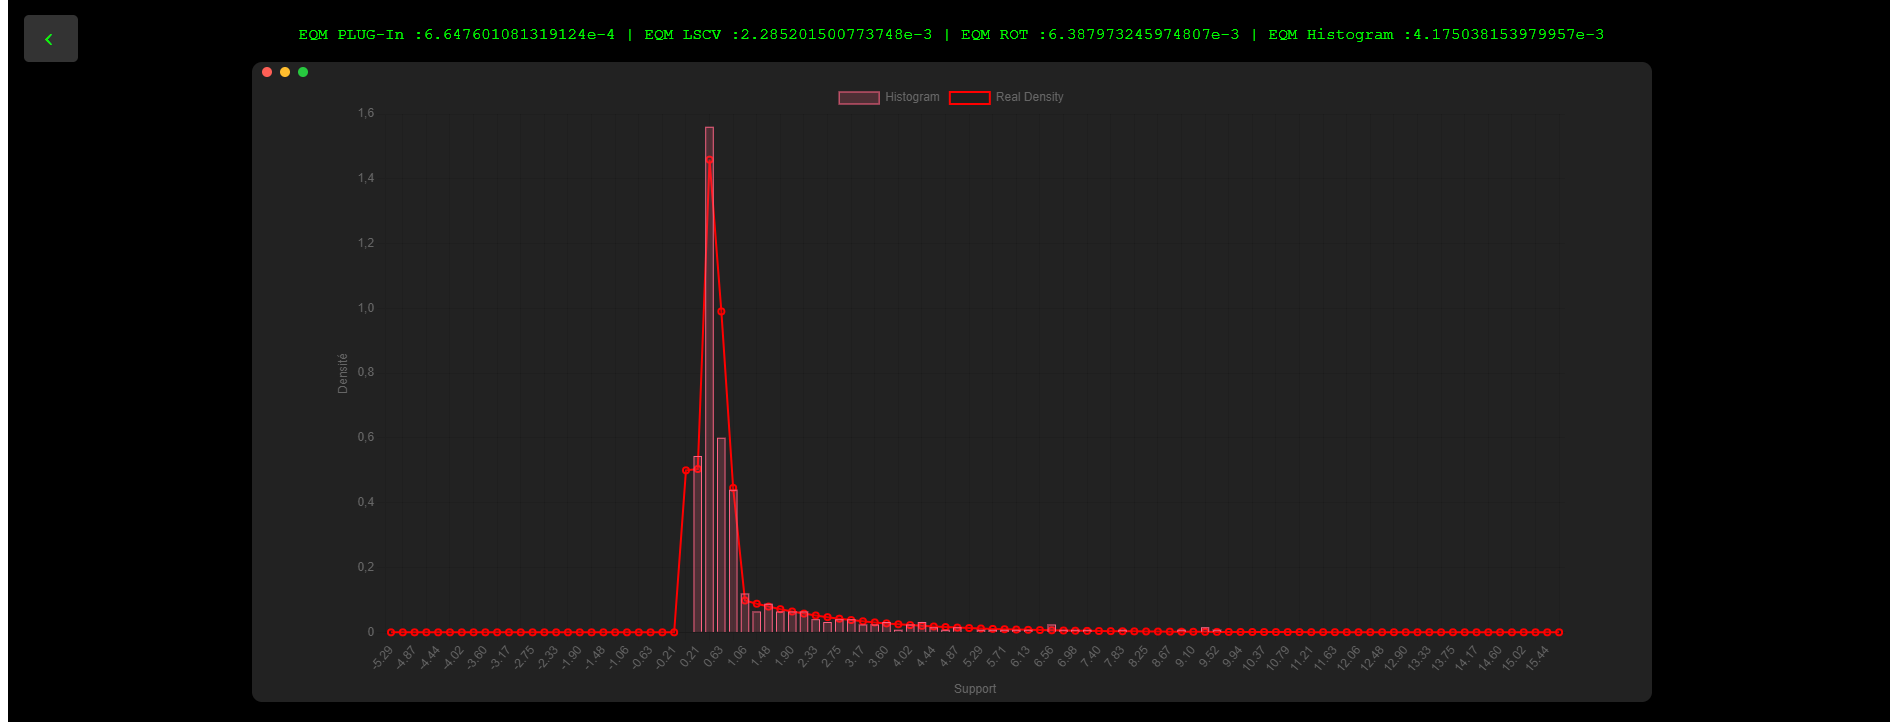
\includegraphics[width=15cm,height=9cm]{Figure 5.4.png}
  \caption{Résultat des simulations - Simulateur}
  \label{fig:Architecture de l'application}
\end{figure}
\clearpage
Si vous choisissez d'importer vos propres données, vous devez sélectionner des fichiers texte (.txt) contenant les données que vous souhaitez estimer leur densité de probabilités( Figure 5.5). Assurez-vous que les données sont séparées par des points-virgules (;) et évitez d'inclure des espaces blancs. Vous avez la possibilité d'importer plusieurs fichiers et de supprimer un fichier importé si nécessaire. Une fois que vous avez importé vos données, il vous suffit de cliquer sur le bouton "Estimer" pour accéder au graphique affichant les densités de probabilités en utilisant la méthode du noyau avec Plug-in pour la sélection du paramètre de lissage.\\
\begin{figure}[!h]
  \centering
  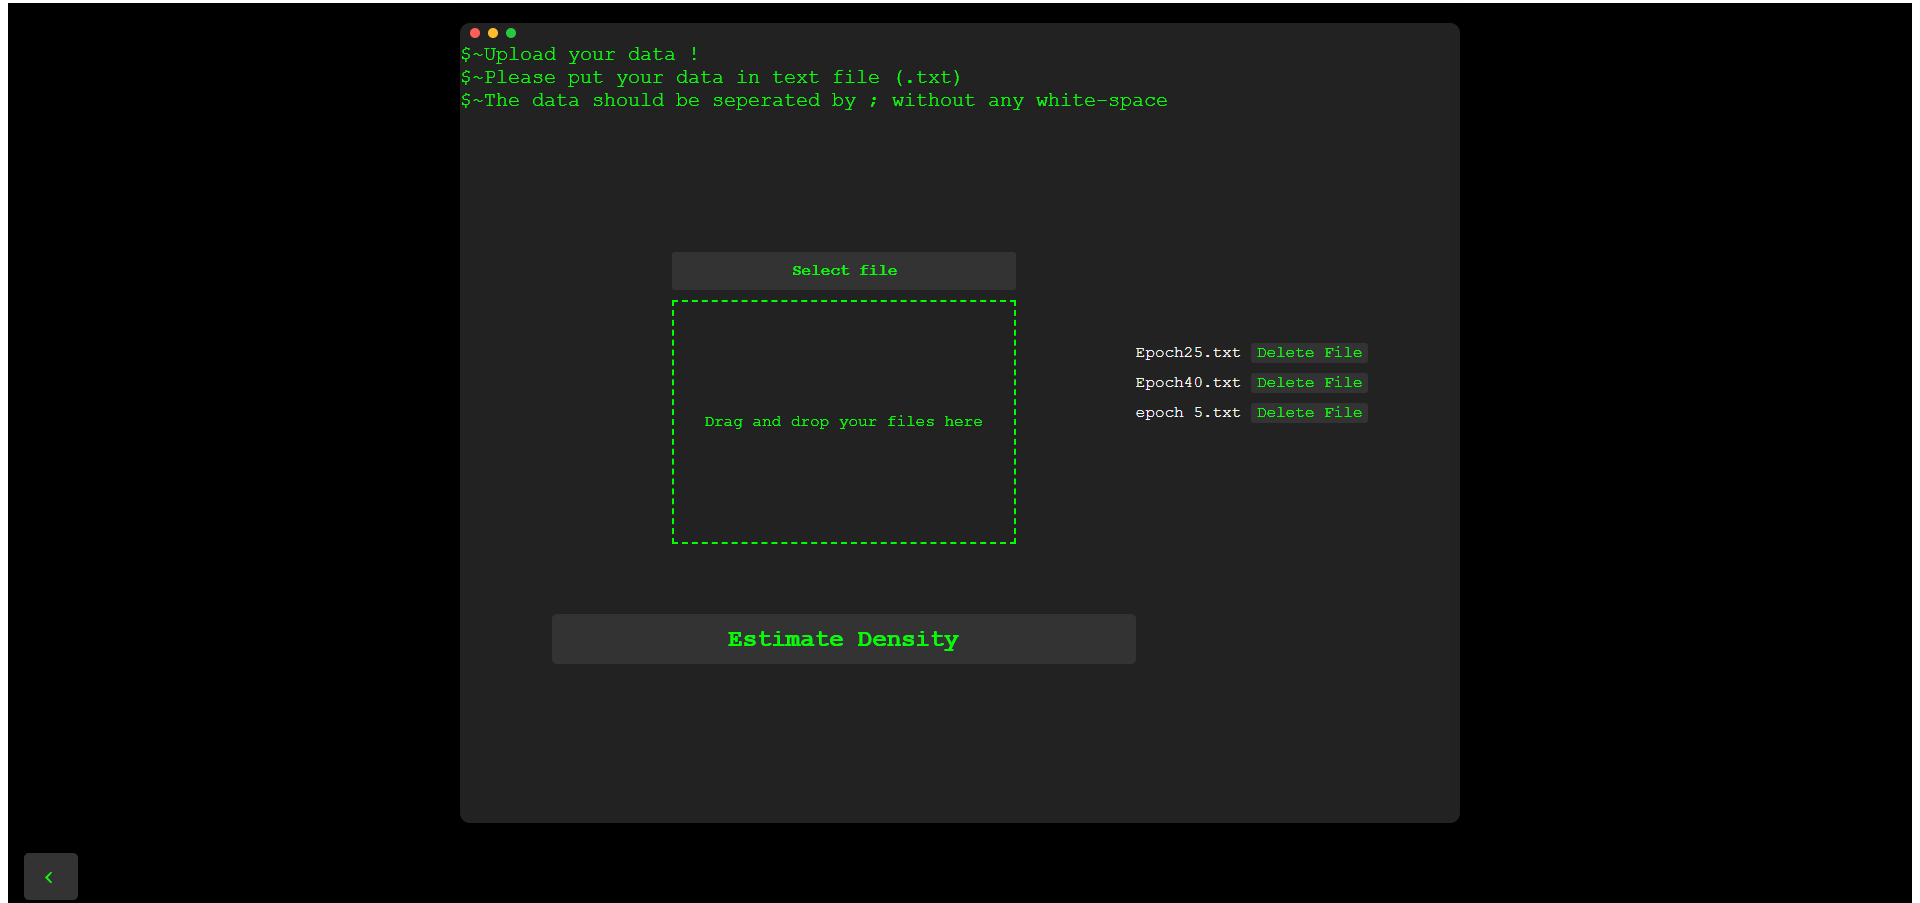
\includegraphics[width=15cm,height=9cm]{Figure 5.5.png}
  \caption{Importation des données - Simulateur}
  \label{fig:Architecture de l'application}
\end{figure}


Dans le graphique ( Figure 5.6), chaque densité de probabilité sera étiquetée avec le nom du fichier correspondant aux données. Toutes les densités seront affichées sur le même graphique, ce qui vous permettra de comparer visuellement les différentes distributions. Vous aurez également la possibilité de cliquer sur l'étiquette de chaque densité pour masquer ou afficher la densité des données d'un fichier spécifique. Cela vous permettra de visualiser sélectivement les densités qui vous intéressent le plus. \\
\begin{figure}[!h]
  \centering
  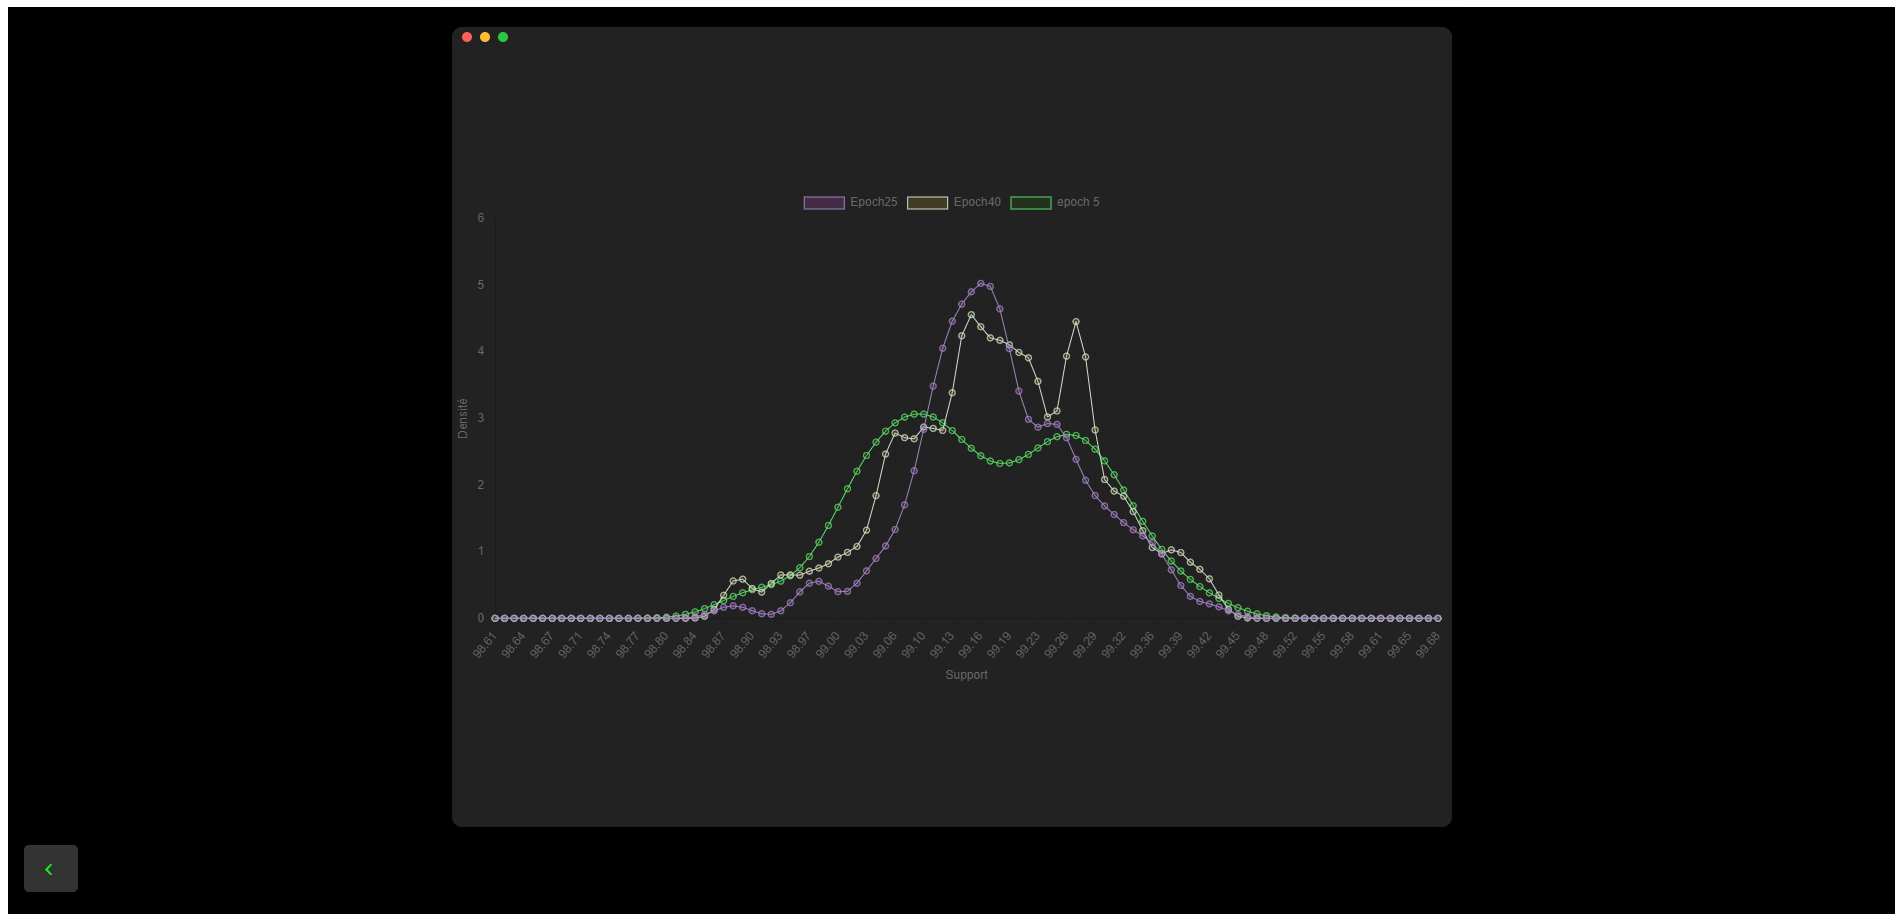
\includegraphics[width=15cm,height=9cm]{Figure 5.6.png}
  \caption{Résultat des estimations - Simulateur}
  \label{fig:Architecture de l'application}
\end{figure}
\newpage
\section{Conclusion}
En conclusion, cette application offre une solution puissante et polyvalente aux chercheurs et informaticiens pour estimer les densités de probabilité des variables aléatoires. Elle constitue un outil essentiel pour comparer les estimateurs et déterminer le meilleur classifieur ou algorithme adapté à leurs besoins.

Pour les chercheurs, cette application leur permet d'explorer et de comparer différents estimateurs, ce qui facilite leur recherche et leur permet de prendre des décisions éclairées en matière d'estimation des densités de probabilité. Ils peuvent ainsi évaluer la performance des estimateurs et identifier celui qui convient le mieux à leur contexte spécifique.

Quant aux informaticiens, cette application leur offre la possibilité d'estimer les densités des variables aléatoires, ce qui leur permet de mieux comprendre et analyser les données. Ils peuvent ainsi prendre des décisions basées sur des informations précises et fiables, notamment dans le cadre du développement de classifieurs et d'algorithmes.

En plus des avantages mentionnés précédemment, cette application offre également des perspectives intéressantes pour son amélioration et son évolution continue. Deux aspects clés peuvent être envisagés pour développer davantage cette application.

Tout d'abord, en ce qui concerne la partie simulation, il est possible d'ajouter d'autres lois de probabilité pour générer des données simulées. Cela élargirait la gamme de distributions disponibles et offrirait une flexibilité supplémentaire pour les expérimentations et les analyses.

Deuxièmement, en ce qui concerne les estimateurs de densité, il serait intéressant de permettre aux utilisateurs de choisir librement les paramètres de lissage pour des estimateurs tels que l'histogramme ou le noyau. Cette fonctionnalité permettrait aux utilisateurs d'explorer et de visualiser l'impact du paramètre de lissage sur les estimations de densité, mettant ainsi en évidence l'influence de ce paramètre sur la précision et la lissage de la courbe estimée.
\clearpage
\chapter*{Conclusion et perspectives}
\addcontentsline{toc}{chapter}{Conclusion et perspectives}
\markboth{Conclusion et perspectives}{Conclusion et perspectives}
\label{sec:conclusion}

Dans ce rapport de recherche, nous avons proposé l'intégration des méthodes d'estimation non paramétriques dans le monde de l'apprentissage automatique pour optimiser et trouver le nombre optimal d'époques pour de meilleures performances et nous avons développé une métrique capable d'évaluer de manière objective la performance des classifieurs.\\
Ce chapitre résume d'abord les travaux proposés, puis une discussion sur les enjeux et contributions de la recherche est présentée, avec des pistes de travaux futurs.
\section*{Conclusion}
En conclusion, notre travail de recherche a permis de mettre en lumière l'importance des méthodes d'estimation non paramétriques dans le domaine de l'apprentissage automatique, en particulier pour l'optimisation de la valeur du nombre d'époques pour obtenir des performances de modèles supérieures. Nous avons réalisé plusieurs simulations pour évaluer la performance des différentes méthodes non paramétriques, afin de sélectionner la plus adaptée à notre problème. De plus, nous avons développé une métrique qui se base sur les densités de probabilité des variables, capable d'évaluer de manière objective la performance des classifieurs.
\setlength{\parindent}{0pt}
Nous avons également présenté un exemple pratique d'application des méthodes paramétriques dans le contexte de l'apprentissage automatique. Ce travail contribue ainsi à l'amélioration de la qualité des modèles en machine learning et peut avoir des applications dans divers domaines, tels que la reconnaissance de forme, la prédiction de séries temporelles, la classification d'images, etc. Enfin, des travaux futurs pourraient inclure l'exploration d'autres méthodes non paramétriques et l'évaluation de leur performance, ainsi que l'application de ces méthodes à d'autres problèmes en apprentissage automatique.
\section*{Perspectives}
 Des améliorations peuvent être apportées à notre travail, en particulier en ce qui concerne la gestion des données et des ressources avec beaucoup de bruit. Nous pourrions également explorer d'autres méthodes non paramétriques et évaluer leurs performances, ainsi qu'appliquer ces méthodes à d'autres problèmes en apprentissage automatique.
\setlength{\parindent}{0pt}
 Enfin, nous pourrions envisager d'intégrer des techniques hybrides de recommandation pour améliorer davantage notre système et lui permettre de fournir des résultats plus précis et personnalisés.





%%%% fin macro %%%%

%%%% fin macro %%%%


 
%%%% fin macro %%%%

%\addstarredchapter{Appendix}


%\appendix

%\chapter{Appendix 1}
\section{Introduction}
Fuzzy set theory was introduced, in 1965, by Zadeh
\cite{fuzzysets}. It is considered as a useful theory for modeling
and reasoning with imprecise knowledge. Fuzzy set theory is a mathematical theory where the fuzziness
is the ambiguity that can be found in the definition of a
concept or the meaning of a word \cite{7f}. Imprecision in
expressions like ``low frequency", ``high demand" or ``small
number" can be called fuzziness. In this Appendix, the basics of fuzzy sets will be introduced. 

In Section A.2, the basics of fuzzy set theory will be given. In Section A.3, the main notions of the fuzzy set membership functions will be introduced while in Section A.4, the fundamental operations of fuzzy sets will be highlighted. Finally, in Section A.5, the process of fuzzy logic will be described.

\section{Conclusion}
In this Appendix, we have elucidated the basics of fuzzy set
theory which is a generalization of the classical set theory.
Offering a natural model,  fuzzy sets are used to handle imprecise information.



%%%% fin macro %%%%



%\nocite{*}

\bibliographystyle{apacite}
\bibliography{NewBib}
\newpage
\thispagestyle{empty}


 

\end{document}